\documentclass[twoside]{book}

% Packages required by doxygen
\usepackage{fixltx2e}
\usepackage{calc}
\usepackage{doxygen}
\usepackage[export]{adjustbox} % also loads graphicx
\usepackage{graphicx}
\usepackage[utf8]{inputenc}
\usepackage{makeidx}
\usepackage{multicol}
\usepackage{multirow}
\PassOptionsToPackage{warn}{textcomp}
\usepackage{textcomp}
\usepackage[nointegrals]{wasysym}
\usepackage[table]{xcolor}

% Font selection
\usepackage[T1]{fontenc}
\usepackage[scaled=.90]{helvet}
\usepackage{courier}
\usepackage{amssymb}
\usepackage{sectsty}
\renewcommand{\familydefault}{\sfdefault}
\allsectionsfont{%
  \fontseries{bc}\selectfont%
  \color{darkgray}%
}
\renewcommand{\DoxyLabelFont}{%
  \fontseries{bc}\selectfont%
  \color{darkgray}%
}
\newcommand{\+}{\discretionary{\mbox{\scriptsize$\hookleftarrow$}}{}{}}

% Page & text layout
\usepackage{geometry}
\geometry{%
  a4paper,%
  top=2.5cm,%
  bottom=2.5cm,%
  left=2.5cm,%
  right=2.5cm%
}
\tolerance=750
\hfuzz=15pt
\hbadness=750
\setlength{\emergencystretch}{15pt}
\setlength{\parindent}{0cm}
\setlength{\parskip}{0.2cm}
\makeatletter
\renewcommand{\paragraph}{%
  \@startsection{paragraph}{4}{0ex}{-1.0ex}{1.0ex}{%
    \normalfont\normalsize\bfseries\SS@parafont%
  }%
}
\renewcommand{\subparagraph}{%
  \@startsection{subparagraph}{5}{0ex}{-1.0ex}{1.0ex}{%
    \normalfont\normalsize\bfseries\SS@subparafont%
  }%
}
\makeatother

% Headers & footers
\usepackage{fancyhdr}
\pagestyle{fancyplain}
\fancyhead[LE]{\fancyplain{}{\bfseries\thepage}}
\fancyhead[CE]{\fancyplain{}{}}
\fancyhead[RE]{\fancyplain{}{\bfseries\leftmark}}
\fancyhead[LO]{\fancyplain{}{\bfseries\rightmark}}
\fancyhead[CO]{\fancyplain{}{}}
\fancyhead[RO]{\fancyplain{}{\bfseries\thepage}}
\fancyfoot[LE]{\fancyplain{}{}}
\fancyfoot[CE]{\fancyplain{}{}}
\fancyfoot[RE]{\fancyplain{}{\bfseries\scriptsize Generated by Doxygen }}
\fancyfoot[LO]{\fancyplain{}{\bfseries\scriptsize Generated by Doxygen }}
\fancyfoot[CO]{\fancyplain{}{}}
\fancyfoot[RO]{\fancyplain{}{}}
\renewcommand{\footrulewidth}{0.4pt}
\renewcommand{\chaptermark}[1]{%
  \markboth{#1}{}%
}
\renewcommand{\sectionmark}[1]{%
  \markright{\thesection\ #1}%
}

% Indices & bibliography
\usepackage{natbib}
\usepackage[titles]{tocloft}
\setcounter{tocdepth}{3}
\setcounter{secnumdepth}{5}
\makeindex

% Hyperlinks (required, but should be loaded last)
\usepackage{ifpdf}
\ifpdf
  \usepackage[pdftex,pagebackref=true]{hyperref}
\else
  \usepackage[ps2pdf,pagebackref=true]{hyperref}
\fi
\hypersetup{%
  colorlinks=true,%
  linkcolor=blue,%
  citecolor=blue,%
  unicode%
}

% Custom commands
\newcommand{\clearemptydoublepage}{%
  \newpage{\pagestyle{empty}\cleardoublepage}%
}


%===== C O N T E N T S =====

\begin{document}

% Titlepage & ToC
\hypersetup{pageanchor=false,
             bookmarks=true,
             bookmarksnumbered=true,
             pdfencoding=unicode
            }
\pagenumbering{roman}
\begin{titlepage}
\vspace*{7cm}
\begin{center}%
{\Large Project Glex }\\
\vspace*{1cm}
{\large Generated by Doxygen 1.8.10}\\
\end{center}
\end{titlepage}
\clearemptydoublepage
\tableofcontents
\clearemptydoublepage
\pagenumbering{arabic}
\hypersetup{pageanchor=true}

%--- Begin generated contents ---
\chapter{Links}
\label{md_Evidence_Of_Glex_Links}
\hypertarget{md_Evidence_Of_Glex_Links}{}
\section*{Youtube Videos}

Camera Evidence \begin{quote}
\href{https://www.youtube.com/watch?v=PtNQCAHK1c0}{\tt https\+://www.\+youtube.\+com/watch?v=\+Pt\+N\+Q\+C\+A\+H\+K1c0} \href{https://www.youtube.com/watch?v=R2AnbXL41hM}{\tt https\+://www.\+youtube.\+com/watch?v=\+R2\+Anb\+X\+L41h\+M}\end{quote}

\chapter{Build Status}
\label{md_README}
\hypertarget{md_README}{}
\href{https://travis-ci.org/Gunn3r1995/glex}{\tt !\mbox{[}Build Status\mbox{]}(https\+://travis-\/ci.\+org/\+Gunn3r1995/glex.\+svg?branch=master)}

\section*{Prerequisites}


\begin{DoxyItemize}
\item G\+N\+U Autotools
\item Open\+G\+L 3.\+0
\item C++11 compiler (tested with G\+C\+C 4.\+8.\+3+)
\item \href{http://www.boost.org/}{\tt Boost}
\item \href{http://glew.sourceforge.net/}{\tt G\+L\+E\+W}
\item \href{https://www.libsdl.org/}{\tt S\+D\+L2}
\item \href{http://glm.g-truc.net/}{\tt G\+L\+M}
\end{DoxyItemize}

On Fedora 20 or later you can install these using a single command (as root)\+:

\begin{quote}
\$ yum install boost-\/$\ast$ glew-\/devel S\+D\+L2\+\_\+$\ast$ glm-\/devel \end{quote}


\section*{Building}

After cloning the source code or extracting a distributed archive, change to the directory where the source code is\+:


\begin{DoxyCode}
1 $ autoreconf -i
2 $ ./configure
3 $ make
\end{DoxyCode}


Alternatively, if you\textquotesingle{}d like to build the project in debug mode use\+:

\begin{quote}
\$ make C\+X\+X\+F\+L\+A\+G\+S=-\/\+D\+D\+E\+B\+U\+G \end{quote}


\section*{Running}

The build process should create a binary that can be executed as follows\+:

\begin{quote}
\$ ./src/shaderexample \end{quote}


See

\begin{quote}
\$ ./src/shaderexample --help \end{quote}


for usage instructions. 
\chapter{Hierarchical Index}
\section{Class Hierarchy}
This inheritance list is sorted roughly, but not completely, alphabetically\+:\begin{DoxyCompactList}
\item \contentsline{section}{Bounding\+Box}{\pageref{class_bounding_box}}{}
\item \contentsline{section}{Camera}{\pageref{class_camera}}{}
\item \contentsline{section}{Game\+Asset}{\pageref{class_game_asset}}{}
\begin{DoxyCompactList}
\item \contentsline{section}{Cube\+Asset}{\pageref{class_cube_asset}}{}
\item \contentsline{section}{Diamond\+Asset}{\pageref{class_diamond_asset}}{}
\item \contentsline{section}{Grass\+Asset}{\pageref{class_grass_asset}}{}
\item \contentsline{section}{Ground\+Asset}{\pageref{class_ground_asset}}{}
\item \contentsline{section}{Leaves\+Asset}{\pageref{class_leaves_asset}}{}
\item \contentsline{section}{Pyramid\+Asset}{\pageref{class_pyramid_asset}}{}
\end{DoxyCompactList}
\item \contentsline{section}{Game\+Asset\+Manager}{\pageref{class_game_asset_manager}}{}
\item \contentsline{section}{Game\+Loop}{\pageref{class_game_loop}}{}
\item \contentsline{section}{Game\+World}{\pageref{class_game_world}}{}
\item \contentsline{section}{Python\+Bind}{\pageref{class_python_bind}}{}
\item \contentsline{section}{S\+D\+L\+Window\+Deleter}{\pageref{struct_s_d_l_window_deleter}}{}
\end{DoxyCompactList}

\chapter{Class Index}
\section{Class List}
Here are the classes, structs, unions and interfaces with brief descriptions\+:\begin{DoxyCompactList}
\item\contentsline{section}{\hyperlink{class_bounding_box}{Bounding\+Box} }{\pageref{class_bounding_box}}{}
\item\contentsline{section}{\hyperlink{class_camera}{Camera} }{\pageref{class_camera}}{}
\item\contentsline{section}{\hyperlink{class_cube_asset}{Cube\+Asset} }{\pageref{class_cube_asset}}{}
\item\contentsline{section}{\hyperlink{class_diamond_asset}{Diamond\+Asset} }{\pageref{class_diamond_asset}}{}
\item\contentsline{section}{\hyperlink{class_game_asset}{Game\+Asset} }{\pageref{class_game_asset}}{}
\item\contentsline{section}{\hyperlink{class_game_asset_manager}{Game\+Asset\+Manager} }{\pageref{class_game_asset_manager}}{}
\item\contentsline{section}{\hyperlink{class_game_loop}{Game\+Loop} }{\pageref{class_game_loop}}{}
\item\contentsline{section}{\hyperlink{class_game_world}{Game\+World} }{\pageref{class_game_world}}{}
\item\contentsline{section}{\hyperlink{class_grass_asset}{Grass\+Asset} }{\pageref{class_grass_asset}}{}
\item\contentsline{section}{\hyperlink{class_ground_asset}{Ground\+Asset} }{\pageref{class_ground_asset}}{}
\item\contentsline{section}{\hyperlink{class_leaves_asset}{Leaves\+Asset} }{\pageref{class_leaves_asset}}{}
\item\contentsline{section}{\hyperlink{class_pyramid_asset}{Pyramid\+Asset} }{\pageref{class_pyramid_asset}}{}
\item\contentsline{section}{\hyperlink{class_python_bind}{Python\+Bind} }{\pageref{class_python_bind}}{}
\item\contentsline{section}{\hyperlink{struct_s_d_l_window_deleter}{S\+D\+L\+Window\+Deleter} }{\pageref{struct_s_d_l_window_deleter}}{}
\end{DoxyCompactList}

\chapter{File Index}
\section{File List}
Here is a list of all files with brief descriptions\+:\begin{DoxyCompactList}
\item\contentsline{section}{\hyperlink{config_8h}{config.\+h} }{\pageref{config_8h}}{}
\item\contentsline{section}{src/\hyperlink{common_8h}{common.\+h} }{\pageref{common_8h}}{}
\item\contentsline{section}{src/\hyperlink{CubeAsset_8cc}{Cube\+Asset.\+cc} }{\pageref{CubeAsset_8cc}}{}
\item\contentsline{section}{src/\hyperlink{CubeAsset_8h}{Cube\+Asset.\+h} }{\pageref{CubeAsset_8h}}{}
\item\contentsline{section}{src/\hyperlink{DiamondAsset_8cc}{Diamond\+Asset.\+cc} }{\pageref{DiamondAsset_8cc}}{}
\item\contentsline{section}{src/\hyperlink{DiamondAsset_8h}{Diamond\+Asset.\+h} }{\pageref{DiamondAsset_8h}}{}
\item\contentsline{section}{src/\hyperlink{GameAsset_8h}{Game\+Asset.\+h} }{\pageref{GameAsset_8h}}{}
\item\contentsline{section}{src/\hyperlink{GameAssetManager_8cc}{Game\+Asset\+Manager.\+cc} }{\pageref{GameAssetManager_8cc}}{}
\item\contentsline{section}{src/\hyperlink{GameAssetManager_8h}{Game\+Asset\+Manager.\+h} }{\pageref{GameAssetManager_8h}}{}
\item\contentsline{section}{src/\hyperlink{GameWorld_8cc}{Game\+World.\+cc} }{\pageref{GameWorld_8cc}}{}
\item\contentsline{section}{src/\hyperlink{GameWorld_8h}{Game\+World.\+h} }{\pageref{GameWorld_8h}}{}
\item\contentsline{section}{src/\hyperlink{GrassAsset_8cc}{Grass\+Asset.\+cc} }{\pageref{GrassAsset_8cc}}{}
\item\contentsline{section}{src/\hyperlink{GrassAsset_8h}{Grass\+Asset.\+h} }{\pageref{GrassAsset_8h}}{}
\item\contentsline{section}{src/\hyperlink{GroundAsset_8cc}{Ground\+Asset.\+cc} }{\pageref{GroundAsset_8cc}}{}
\item\contentsline{section}{src/\hyperlink{GroundAsset_8h}{Ground\+Asset.\+h} }{\pageref{GroundAsset_8h}}{}
\item\contentsline{section}{src/\hyperlink{LeavesAsset_8cc}{Leaves\+Asset.\+cc} }{\pageref{LeavesAsset_8cc}}{}
\item\contentsline{section}{src/\hyperlink{LeavesAsset_8h}{Leaves\+Asset.\+h} }{\pageref{LeavesAsset_8h}}{}
\item\contentsline{section}{src/\hyperlink{main_8cc}{main.\+cc} }{\pageref{main_8cc}}{}
\item\contentsline{section}{src/\hyperlink{PyramidAsset_8cc}{Pyramid\+Asset.\+cc} }{\pageref{PyramidAsset_8cc}}{}
\item\contentsline{section}{src/\hyperlink{PyramidAsset_8h}{Pyramid\+Asset.\+h} }{\pageref{PyramidAsset_8h}}{}
\end{DoxyCompactList}

\chapter{Class Documentation}
\hypertarget{classCubeAsset}{}\section{Cube\+Asset Class Reference}
\label{classCubeAsset}\index{Cube\+Asset@{Cube\+Asset}}


{\ttfamily \#include $<$Cube\+Asset.\+h$>$}



Inheritance diagram for Cube\+Asset\+:\nopagebreak
\begin{figure}[H]
\begin{center}
\leavevmode
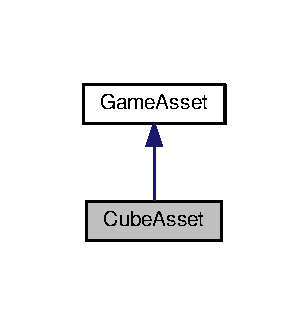
\includegraphics[width=148pt]{classCubeAsset__inherit__graph}
\end{center}
\end{figure}


Collaboration diagram for Cube\+Asset\+:\nopagebreak
\begin{figure}[H]
\begin{center}
\leavevmode
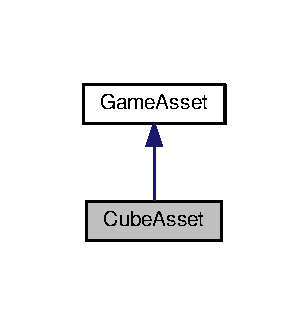
\includegraphics[width=148pt]{classCubeAsset__coll__graph}
\end{center}
\end{figure}
\subsection*{Public Member Functions}
\begin{DoxyCompactItemize}
\item 
\hyperlink{classCubeAsset_a0252e564114a3cda7e3911ef95742a34}{Cube\+Asset} (G\+Lfloat x, G\+Lfloat y, G\+Lfloat z)
\item 
\hyperlink{classCubeAsset_ab3ab9a5da82cbf8537a28652410093b1}{$\sim$\+Cube\+Asset} ()
\item 
virtual void \hyperlink{classCubeAsset_a1af568486056e254ffcf98fd99947bfe}{Draw} (G\+Luint)
\end{DoxyCompactItemize}


\subsection{Constructor \& Destructor Documentation}
\hypertarget{classCubeAsset_a0252e564114a3cda7e3911ef95742a34}{}\index{Cube\+Asset@{Cube\+Asset}!Cube\+Asset@{Cube\+Asset}}
\index{Cube\+Asset@{Cube\+Asset}!Cube\+Asset@{Cube\+Asset}}
\subsubsection[{Cube\+Asset(\+G\+Lfloat x, G\+Lfloat y, G\+Lfloat z)}]{\setlength{\rightskip}{0pt plus 5cm}Cube\+Asset\+::\+Cube\+Asset (
\begin{DoxyParamCaption}
\item[{G\+Lfloat}]{x, }
\item[{G\+Lfloat}]{y, }
\item[{G\+Lfloat}]{z}
\end{DoxyParamCaption}
)}\label{classCubeAsset_a0252e564114a3cda7e3911ef95742a34}
model coordinates, origin at centre. Sets cordinates to a cube with the center point 0.\+0 but moved to where the x, y, z variables calls them from the gameworld class through the G\+Lfloat x,y,z variables.

Color Buffer. Colour of Cube Asset Saddle Brown Uses R\+G\+B values to set the colour.

Element buffer. Draws the cube voxel up of 12 Triangles Two Triangles per Face.
\begin{DoxyCode}
3                                                      \{
4 
11   GLfloat vertex\_buffer [] \{
12       0.5f + x  , 0.5f + y  , -0.5f + z
13     , 0.5f + x  ,-0.5f + y  , -0.5f + z
14     ,-0.5f + x  , 0.5f + y  , -0.5f + z
15     ,-0.5f + x  ,-0.5f + y  , -0.5f + z
16     , 0.5f + x  , 0.5f + y  ,  0.5f + z 
17     , 0.5f + x  ,-0.5f + y  ,  0.5f + z
18     ,-0.5f + x  , 0.5f + y  ,  0.5f + z
19     ,-0.5f + x  ,-0.5f + y  ,  0.5f + z
20   \};
21   GLfloat vertex\_buffer\_length = \textcolor{keyword}{sizeof}(vertex\_buffer);
27   GLfloat colour\_buffer[] = \{
28 
29      0.139f, 0.069f, 0.019f,
30      0.139f, 0.069f, 0.019f,
31      0.139f, 0.069f, 0.019f,
32      0.139f, 0.069f, 0.019f,
33      0.139f, 0.069f, 0.019f,
34      0.139f, 0.069f, 0.019f,
35      0.139f, 0.069f, 0.019f,
36      0.139f, 0.069f, 0.019f
37   \};
38   colour\_buffer\_length = \textcolor{keyword}{sizeof}(colour\_buffer);
44   GLuint element\_buffer []  \{
45       0, 1, 2   
46     , 1, 3, 2
47     , 0, 4, 1   
48     , 1, 5, 4   
49     , 5, 7, 4   
50     , 7, 6, 4   
51     , 3, 7, 6   
52     , 2, 3, 6   
53     , 1, 5, 7   
54     , 1, 3, 7   
55     , 0, 4, 6   
56     , 0, 2, 6   
57   \};
58   element\_buffer\_length = \textcolor{keyword}{sizeof}(element\_buffer);
59 
60 
61 
62   \textcolor{comment}{// Transfer buffers to the GPU}
63 
64   \textcolor{comment}{// create buffer}
65   glGenBuffers(1, &vertex\_buffer\_token);
66   \textcolor{comment}{// immediately bind the buffer and transfer the data}
67   glBindBuffer(GL\_ARRAY\_BUFFER, vertex\_buffer\_token);
68   glBufferData(GL\_ARRAY\_BUFFER, vertex\_buffer\_length, vertex\_buffer, GL\_STATIC\_DRAW);
69   
70   \textcolor{comment}{// Binds the buffer to transfer the data}
71   glGenBuffers(1, &colour\_buffer\_token);
72   glBindBuffer(GL\_ARRAY\_BUFFER, colour\_buffer\_token);
73   glBufferData(GL\_ARRAY\_BUFFER, colour\_buffer\_length, colour\_buffer, GL\_STATIC\_DRAW);
74 
75 
76   glGenBuffers(1, &element\_buffer\_token);
77   glBindBuffer(GL\_ELEMENT\_ARRAY\_BUFFER, element\_buffer\_token);
78   glBufferData(GL\_ELEMENT\_ARRAY\_BUFFER, element\_buffer\_length, element\_buffer, GL\_STATIC\_DRAW);
79 \}
\end{DoxyCode}
\hypertarget{classCubeAsset_ab3ab9a5da82cbf8537a28652410093b1}{}\index{Cube\+Asset@{Cube\+Asset}!````~Cube\+Asset@{$\sim$\+Cube\+Asset}}
\index{````~Cube\+Asset@{$\sim$\+Cube\+Asset}!Cube\+Asset@{Cube\+Asset}}
\subsubsection[{$\sim$\+Cube\+Asset()}]{\setlength{\rightskip}{0pt plus 5cm}Cube\+Asset\+::$\sim$\+Cube\+Asset (
\begin{DoxyParamCaption}
{}
\end{DoxyParamCaption}
)}\label{classCubeAsset_ab3ab9a5da82cbf8537a28652410093b1}

\begin{DoxyCode}
81                       \{
82 \}
\end{DoxyCode}


\subsection{Member Function Documentation}
\hypertarget{classCubeAsset_a1af568486056e254ffcf98fd99947bfe}{}\index{Cube\+Asset@{Cube\+Asset}!Draw@{Draw}}
\index{Draw@{Draw}!Cube\+Asset@{Cube\+Asset}}
\subsubsection[{Draw(\+G\+Luint)}]{\setlength{\rightskip}{0pt plus 5cm}void Cube\+Asset\+::\+Draw (
\begin{DoxyParamCaption}
\item[{G\+Luint}]{program\+\_\+token}
\end{DoxyParamCaption}
)\hspace{0.3cm}{\ttfamily [virtual]}}\label{classCubeAsset_a1af568486056e254ffcf98fd99947bfe}
use the previously transferred buffer as the vertex array. This way we transfer the buffer once -- at construction -- not on every frame.

Uses the Previously transferred buffer as the color array. This way We transfer the buffer once -- at constuction -- not on every frame

Implements \hyperlink{classGameAsset_a961aa51ca0a9961fc584c0b5d5431300}{Game\+Asset}.


\begin{DoxyCode}
99                                          \{
100   \textcolor{keywordflow}{if}(!glIsProgram(program\_token)) \{
101     std::cerr << \textcolor{stringliteral}{"Drawing Cube with invalid program"} << std::endl;
102     \textcolor{keywordflow}{return};
103   \}
104   GLint validation\_ok;
105   glValidateProgram(program\_token);
106   glGetProgramiv(program\_token, GL\_VALIDATE\_STATUS, &validation\_ok);
107   \textcolor{keywordflow}{if}(!validation\_ok) \{
108     GLint maxLength = 0;
109     glGetProgramiv(program\_token, GL\_INFO\_LOG\_LENGTH, &maxLength);
110 
111     \textcolor{comment}{// The maxLength includes the NULL character}
112     std::vector<char> errorLog(maxLength);
113     glGetProgramInfoLog(program\_token, maxLength, &maxLength, &errorLog[0]);
114 
115     std::cerr << \textcolor{stringliteral}{"Invalid program "} << program\_token << \textcolor{stringliteral}{" with error code "} << validation\_ok << std::endl;
116     \textcolor{keywordflow}{for}(\textcolor{keyword}{auto} c: errorLog) \{
117       std::cerr << c;
118     \}
119     exit(-1);
120   \}
121 
122   GLuint position\_attrib = glGetAttribLocation(program\_token, \textcolor{stringliteral}{"position"});
123   \hyperlink{CubeAsset_8cc_a75f201b0e53e68726854997957322b8d}{checkGLError}();
124 
125   glUseProgram(program\_token);
126   \hyperlink{CubeAsset_8cc_a75f201b0e53e68726854997957322b8d}{checkGLError}();
131   glEnableVertexAttribArray(0);
132   glBindBuffer(GL\_ARRAY\_BUFFER, vertex\_buffer\_token);
133   glVertexAttribPointer(
134     position\_attrib,        \textcolor{comment}{/* attribute */}
135     3,        \textcolor{comment}{/* size */}
136     GL\_FLOAT,   \textcolor{comment}{/* type */}
137     GL\_FALSE,   \textcolor{comment}{/* normalized? */}
138     0,        \textcolor{comment}{/* stride */}
139     (\textcolor{keywordtype}{void}*)0    \textcolor{comment}{/* array buffer offset */}
140   );
141   glEnableVertexAttribArray(1);
142   \hyperlink{CubeAsset_8cc_a75f201b0e53e68726854997957322b8d}{checkGLError}();
147   glBindBuffer(GL\_ARRAY\_BUFFER, colour\_buffer\_token);
148   glVertexAttribPointer(
149     1,        \textcolor{comment}{/* attribute */}
150     3,        \textcolor{comment}{/* size */}
151     GL\_FLOAT,   \textcolor{comment}{/* type */}
152     GL\_FALSE,   \textcolor{comment}{/* normalized? */}
153     0,        \textcolor{comment}{/* stride */}
154     (\textcolor{keywordtype}{void}*)0    \textcolor{comment}{/* array buffer offset */}
155   );
156   \hyperlink{CubeAsset_8cc_a75f201b0e53e68726854997957322b8d}{checkGLError}();
157 
158   glBindBuffer(GL\_ELEMENT\_ARRAY\_BUFFER, element\_buffer\_token);
159   glDrawElements(
160     GL\_TRIANGLES,
161     element\_buffer\_length,
162     GL\_UNSIGNED\_INT,
163     (GLvoid*) 0
164   );
165   \hyperlink{CubeAsset_8cc_a75f201b0e53e68726854997957322b8d}{checkGLError}();
166 
167   glDisableVertexAttribArray(position\_attrib);
168 \}
\end{DoxyCode}


The documentation for this class was generated from the following files\+:\begin{DoxyCompactItemize}
\item 
src/\hyperlink{CubeAsset_8h}{Cube\+Asset.\+h}\item 
src/\hyperlink{CubeAsset_8cc}{Cube\+Asset.\+cc}\end{DoxyCompactItemize}

\hypertarget{classDiamondAsset}{}\section{Diamond\+Asset Class Reference}
\label{classDiamondAsset}\index{Diamond\+Asset@{Diamond\+Asset}}


{\ttfamily \#include $<$Diamond\+Asset.\+h$>$}



Inheritance diagram for Diamond\+Asset\+:\nopagebreak
\begin{figure}[H]
\begin{center}
\leavevmode
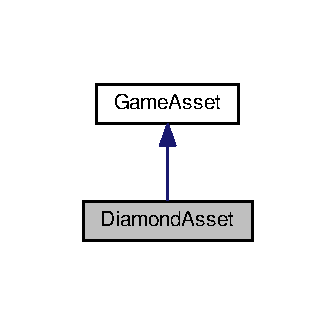
\includegraphics[width=161pt]{classDiamondAsset__inherit__graph}
\end{center}
\end{figure}


Collaboration diagram for Diamond\+Asset\+:\nopagebreak
\begin{figure}[H]
\begin{center}
\leavevmode
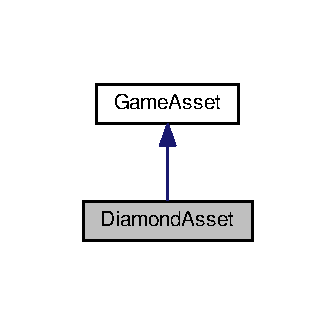
\includegraphics[width=161pt]{classDiamondAsset__coll__graph}
\end{center}
\end{figure}
\subsection*{Public Member Functions}
\begin{DoxyCompactItemize}
\item 
\hyperlink{classDiamondAsset_a6140b65eb30ad5a4141fec20ec7f8fad}{Diamond\+Asset} (G\+Lfloat x, G\+Lfloat y, G\+Lfloat z)
\item 
\hyperlink{classDiamondAsset_a1b7bf6ba76651a9304943f2c41fe36b8}{$\sim$\+Diamond\+Asset} ()
\item 
virtual void \hyperlink{classDiamondAsset_a0c259031894623285b3b511321c73abb}{Draw} (G\+Luint)
\item 
void \hyperlink{classDiamondAsset_ad0eafff97cf565024dd085f3c8786a93}{check\+Error} (std\+::string file, int line)
\end{DoxyCompactItemize}


\subsection{Constructor \& Destructor Documentation}
\hypertarget{classDiamondAsset_a6140b65eb30ad5a4141fec20ec7f8fad}{}\index{Diamond\+Asset@{Diamond\+Asset}!Diamond\+Asset@{Diamond\+Asset}}
\index{Diamond\+Asset@{Diamond\+Asset}!Diamond\+Asset@{Diamond\+Asset}}
\subsubsection[{Diamond\+Asset(\+G\+Lfloat x, G\+Lfloat y, G\+Lfloat z)}]{\setlength{\rightskip}{0pt plus 5cm}Diamond\+Asset\+::\+Diamond\+Asset (
\begin{DoxyParamCaption}
\item[{G\+Lfloat}]{x, }
\item[{G\+Lfloat}]{y, }
\item[{G\+Lfloat}]{z}
\end{DoxyParamCaption}
)}\label{classDiamondAsset_a6140b65eb30ad5a4141fec20ec7f8fad}
model coordinates, origin at centre.

Sets cordinates to a diamond with the center point 0.\+0 but moved to where the x, y, z variables calls them

Colour of Diamond Asset Red Uses R\+G\+B values

Draws the Diamond up of 8 Triangles One Triangles per Face

Transfer buffers to the G\+P\+U

create buffer

immediately bind the buffer and transfer the data

Binds the buffer and transfers the data 
\begin{DoxyCode}
4                                                           \{
5 
7 
11   GLfloat vertex\_buffer [] \{
12      -0.5f + x  , 0.0f + y   , 0.0f + z
13      ,0.5f + x  , 0.0f + y   , 0.0f + z
14      ,0.0f + x  ,-0.5f + y   , 0.0f + z
15      ,0.0f + x  , 0.5f + y   , 0.0f + z
16      ,0.0f + x  , 0.0f + y   ,-0.5f + z
17      ,0.0f + x  , 0.0f + y   , 0.5f + z
18   \};
19   GLfloat vertex\_buffer\_length = \textcolor{keyword}{sizeof}(vertex\_buffer);
24   GLfloat colour\_buffer[] = \{
25 
26      1.000f, 0.000f, 0.000f,
27      1.000f, 0.000f, 0.000f,
28      1.000f, 0.000f, 0.000f,
29      1.000f, 0.000f, 0.000f,
30      1.000f, 0.000f, 0.000f,
31      1.000f, 0.000f, 0.000f
32   \};
33   colour\_buffer\_length = \textcolor{keyword}{sizeof}(colour\_buffer);
38   GLuint element\_buffer []  \{
39       0, 3, 5   
40     , 3, 1, 5
41     , 0, 5, 2   
42     , 5, 1, 2
43     , 0, 3, 4
44     , 3, 1, 4
45     , 0, 4, 2
46     , 4, 1, 2
47   \};
48   element\_buffer\_length = \textcolor{keyword}{sizeof}(element\_buffer);
49 
50 
51 
53 
55   glGenBuffers(1, &vertex\_buffer\_token);
57   glBindBuffer(GL\_ARRAY\_BUFFER, vertex\_buffer\_token);
58   glBufferData(GL\_ARRAY\_BUFFER, vertex\_buffer\_length, vertex\_buffer, GL\_STATIC\_DRAW);
59 
61   glGenBuffers(1, &colour\_buffer\_token);
62   glBindBuffer(GL\_ARRAY\_BUFFER, colour\_buffer\_token);
63   glBufferData(GL\_ARRAY\_BUFFER, colour\_buffer\_length, colour\_buffer, GL\_STATIC\_DRAW);
64 
65 
66   glGenBuffers(1, &element\_buffer\_token);
67   glBindBuffer(GL\_ELEMENT\_ARRAY\_BUFFER, element\_buffer\_token);
68   glBufferData(GL\_ELEMENT\_ARRAY\_BUFFER, element\_buffer\_length, element\_buffer, GL\_STATIC\_DRAW);
69 \}
\end{DoxyCode}
\hypertarget{classDiamondAsset_a1b7bf6ba76651a9304943f2c41fe36b8}{}\index{Diamond\+Asset@{Diamond\+Asset}!````~Diamond\+Asset@{$\sim$\+Diamond\+Asset}}
\index{````~Diamond\+Asset@{$\sim$\+Diamond\+Asset}!Diamond\+Asset@{Diamond\+Asset}}
\subsubsection[{$\sim$\+Diamond\+Asset()}]{\setlength{\rightskip}{0pt plus 5cm}Diamond\+Asset\+::$\sim$\+Diamond\+Asset (
\begin{DoxyParamCaption}
{}
\end{DoxyParamCaption}
)}\label{classDiamondAsset_a1b7bf6ba76651a9304943f2c41fe36b8}

\begin{DoxyCode}
71                             \{
72 \}
\end{DoxyCode}


\subsection{Member Function Documentation}
\hypertarget{classDiamondAsset_ad0eafff97cf565024dd085f3c8786a93}{}\index{Diamond\+Asset@{Diamond\+Asset}!check\+Error@{check\+Error}}
\index{check\+Error@{check\+Error}!Diamond\+Asset@{Diamond\+Asset}}
\subsubsection[{check\+Error(std\+::string file, int line)}]{\setlength{\rightskip}{0pt plus 5cm}void Diamond\+Asset\+::check\+Error (
\begin{DoxyParamCaption}
\item[{std\+::string}]{file, }
\item[{int}]{line}
\end{DoxyParamCaption}
)}\label{classDiamondAsset_ad0eafff97cf565024dd085f3c8786a93}

\begin{DoxyCode}
81                                                       \{
82   GLenum gl\_error = glGetError();
83   \textcolor{keywordflow}{if}(GL\_NO\_ERROR != gl\_error) \{
84     std::cerr << \textcolor{stringliteral}{"GL error in "} << file << \textcolor{stringliteral}{" at line "} << line << \textcolor{stringliteral}{" error: "} << gl\_error << std::endl;
85     exit(-1);
86   \}
87 \}
\end{DoxyCode}
\hypertarget{classDiamondAsset_a0c259031894623285b3b511321c73abb}{}\index{Diamond\+Asset@{Diamond\+Asset}!Draw@{Draw}}
\index{Draw@{Draw}!Diamond\+Asset@{Diamond\+Asset}}
\subsubsection[{Draw(\+G\+Luint)}]{\setlength{\rightskip}{0pt plus 5cm}void Diamond\+Asset\+::\+Draw (
\begin{DoxyParamCaption}
\item[{G\+Luint}]{program\+\_\+token}
\end{DoxyParamCaption}
)\hspace{0.3cm}{\ttfamily [virtual]}}\label{classDiamondAsset_a0c259031894623285b3b511321c73abb}
The max\+Length includes the N\+U\+L\+L character

use the previously transferred buffer as the vertex array. This way we transfer the buffer once -- at construction -- not on every frame.

attribute

size

type

normalized?

stride

array buffer offset

Uses the Previously transferred buffer as the color array. This way We transfer the buffer once -- at constuction -- not on every frame

attribute

size

type

normalized?

stride

array buffer offset 

Implements \hyperlink{classGameAsset_a961aa51ca0a9961fc584c0b5d5431300}{Game\+Asset}.


\begin{DoxyCode}
89                                             \{
90   \textcolor{keywordflow}{if}(!glIsProgram(program\_token)) \{
91     std::cerr << \textcolor{stringliteral}{"Drawing Diamond with invalid program"} << std::endl;
92     \textcolor{keywordflow}{return};
93   \}
94   GLint validation\_ok;
95   glValidateProgram(program\_token);
96   glGetProgramiv(program\_token, GL\_VALIDATE\_STATUS, &validation\_ok);
97   \textcolor{keywordflow}{if}(!validation\_ok) \{
98     GLint maxLength = 0;
99     glGetProgramiv(program\_token, GL\_INFO\_LOG\_LENGTH, &maxLength);
100 
102     std::vector<char> errorLog(maxLength);
103     glGetProgramInfoLog(program\_token, maxLength, &maxLength, &errorLog[0]);
104 
105     std::cerr << \textcolor{stringliteral}{"Invalid program "} << program\_token << \textcolor{stringliteral}{" with error code "} << validation\_ok << std::endl;
106     \textcolor{keywordflow}{for}(\textcolor{keyword}{auto} c: errorLog) \{
107       std::cerr << c;
108     \}
109     exit(-1);
110   \}
111 
112   GLuint position\_attrib = glGetAttribLocation(program\_token, \textcolor{stringliteral}{"position"});
113   \hyperlink{DiamondAsset_8cc_a75f201b0e53e68726854997957322b8d}{checkGLError}();
114 
115   glUseProgram(program\_token);
116   \hyperlink{DiamondAsset_8cc_a75f201b0e53e68726854997957322b8d}{checkGLError}();
117 
121   glEnableVertexAttribArray(0);
122   glBindBuffer(GL\_ARRAY\_BUFFER, vertex\_buffer\_token);
123   glVertexAttribPointer(
124     position\_attrib,        
125     3,        
126     GL\_FLOAT,   
127     GL\_FALSE,   
128     0,        
129     (\textcolor{keywordtype}{void}*)0    
130   );
131   glEnableVertexAttribArray(1);
132   \hyperlink{DiamondAsset_8cc_a75f201b0e53e68726854997957322b8d}{checkGLError}();
137   glBindBuffer(GL\_ARRAY\_BUFFER, colour\_buffer\_token);
138   glVertexAttribPointer(
139     1,        
140     3,        
141     GL\_FLOAT,   
142     GL\_FALSE,   
143     0,        
144     (\textcolor{keywordtype}{void}*)0    
145   );
146   \hyperlink{DiamondAsset_8cc_a75f201b0e53e68726854997957322b8d}{checkGLError}();
147 
148   glBindBuffer(GL\_ELEMENT\_ARRAY\_BUFFER, element\_buffer\_token);
149   glDrawElements(
150     GL\_TRIANGLES,
151     element\_buffer\_length,
152     GL\_UNSIGNED\_INT,
153     (GLvoid*) 0
154   );
155   \hyperlink{DiamondAsset_8cc_a75f201b0e53e68726854997957322b8d}{checkGLError}();
156 
157   glDisableVertexAttribArray(position\_attrib);
158 \}
\end{DoxyCode}


The documentation for this class was generated from the following files\+:\begin{DoxyCompactItemize}
\item 
src/\hyperlink{DiamondAsset_8h}{Diamond\+Asset.\+h}\item 
src/\hyperlink{DiamondAsset_8cc}{Diamond\+Asset.\+cc}\end{DoxyCompactItemize}

\hypertarget{classGameAsset}{}\section{Game\+Asset Class Reference}
\label{classGameAsset}\index{Game\+Asset@{Game\+Asset}}


{\ttfamily \#include $<$Game\+Asset.\+h$>$}



Inheritance diagram for Game\+Asset\+:\nopagebreak
\begin{figure}[H]
\begin{center}
\leavevmode
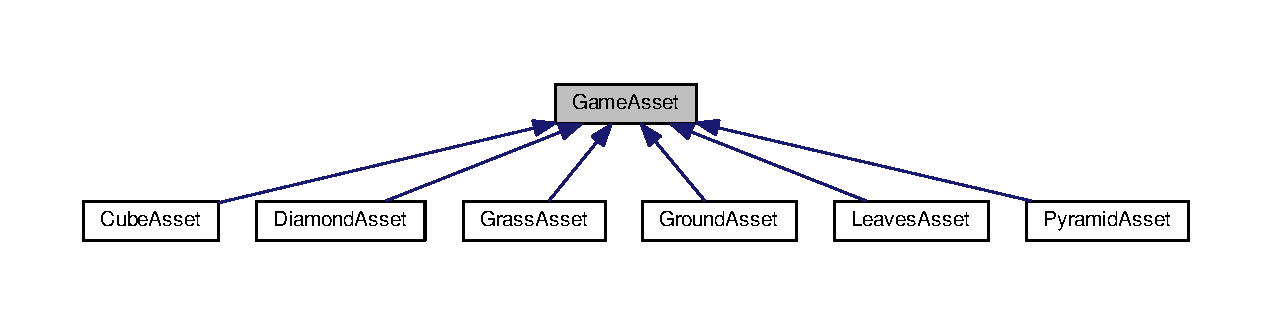
\includegraphics[width=350pt]{classGameAsset__inherit__graph}
\end{center}
\end{figure}
\subsection*{Public Member Functions}
\begin{DoxyCompactItemize}
\item 
virtual void \hyperlink{classGameAsset_a961aa51ca0a9961fc584c0b5d5431300}{Draw} (G\+Luint)=0
\end{DoxyCompactItemize}


\subsection{Member Function Documentation}
\hypertarget{classGameAsset_a961aa51ca0a9961fc584c0b5d5431300}{}\index{Game\+Asset@{Game\+Asset}!Draw@{Draw}}
\index{Draw@{Draw}!Game\+Asset@{Game\+Asset}}
\subsubsection[{Draw(\+G\+Luint)=0}]{\setlength{\rightskip}{0pt plus 5cm}virtual void Game\+Asset\+::\+Draw (
\begin{DoxyParamCaption}
\item[{G\+Luint}]{}
\end{DoxyParamCaption}
)\hspace{0.3cm}{\ttfamily [pure virtual]}}\label{classGameAsset_a961aa51ca0a9961fc584c0b5d5431300}


Implemented in \hyperlink{classCubeAsset_a1af568486056e254ffcf98fd99947bfe}{Cube\+Asset}, \hyperlink{classGrassAsset_a0178a72c5bf2f00bcc6a240b851f3a25}{Grass\+Asset}, \hyperlink{classGroundAsset_a440f983638c7a7ccb6a39718444dfe95}{Ground\+Asset}, \hyperlink{classLeavesAsset_a807fd196b83e5adb131d489ef6645742}{Leaves\+Asset}, \hyperlink{classPyramidAsset_aaea45da4956d79ec9ab96e9d0ccef3fe}{Pyramid\+Asset}, and \hyperlink{classDiamondAsset_a0c259031894623285b3b511321c73abb}{Diamond\+Asset}.



The documentation for this class was generated from the following file\+:\begin{DoxyCompactItemize}
\item 
src/\hyperlink{GameAsset_8h}{Game\+Asset.\+h}\end{DoxyCompactItemize}

\hypertarget{classGameAssetManager}{}\section{Game\+Asset\+Manager Class Reference}
\label{classGameAssetManager}\index{Game\+Asset\+Manager@{Game\+Asset\+Manager}}


{\ttfamily \#include $<$Game\+Asset\+Manager.\+h$>$}

\subsection*{Public Member Functions}
\begin{DoxyCompactItemize}
\item 
\hyperlink{classGameAssetManager_aaa0d58e276cc10ad91a7457085598a71}{Game\+Asset\+Manager} (\hyperlink{common_8h_add86e7c88dd109abea3f708b422f31f0}{Application\+Mode})
\item 
virtual \hyperlink{classGameAssetManager_a1270bd61ecbcca563f079803e40c9b77}{$\sim$\+Game\+Asset\+Manager} ()
\begin{DoxyCompactList}\small\item\em constructor \end{DoxyCompactList}\item 
\hyperlink{classGameAssetManager_a2c9adcb72faa154c87eadc9bafe5269d}{Game\+Asset\+Manager} (\hyperlink{classGameAssetManager}{Game\+Asset\+Manager} const \&)
\item 
\hyperlink{classGameAssetManager_a44f6e2fd6b8ff1dd64e5697f1be7386d}{Game\+Asset\+Manager} (\hyperlink{classGameAssetManager}{Game\+Asset\+Manager} const \&\&)
\begin{DoxyCompactList}\small\item\em copy constructor \end{DoxyCompactList}\item 
void \hyperlink{classGameAssetManager_ac72678a4ad5378c685aa6bae84a4e712}{operator=} (\hyperlink{classGameAssetManager}{Game\+Asset\+Manager} const \&)
\begin{DoxyCompactList}\small\item\em move constructor \end{DoxyCompactList}\item 
void \hyperlink{classGameAssetManager_ad3de8ff00d55ba04728b1de8213b2349}{Add\+Asset} (std\+::shared\+\_\+ptr$<$ \hyperlink{classGameAsset}{Game\+Asset} $>$)
\begin{DoxyCompactList}\small\item\em assignment \end{DoxyCompactList}\item 
void \hyperlink{classGameAssetManager_a32837132bd70a9a9ed537323c2d3d886}{Draw} ()
\end{DoxyCompactItemize}


\subsection{Detailed Description}
\hyperlink{classGameAssetManager}{Game\+Asset\+Manager} is a container for Game\+Assets. It also provides utility functions to to create a simple Open\+G\+L program that can be used to draw a simple \hyperlink{classGameAsset}{Game\+Asset}. 

\subsection{Constructor \& Destructor Documentation}
\hypertarget{classGameAssetManager_aaa0d58e276cc10ad91a7457085598a71}{}\index{Game\+Asset\+Manager@{Game\+Asset\+Manager}!Game\+Asset\+Manager@{Game\+Asset\+Manager}}
\index{Game\+Asset\+Manager@{Game\+Asset\+Manager}!Game\+Asset\+Manager@{Game\+Asset\+Manager}}
\subsubsection[{Game\+Asset\+Manager(\+Application\+Mode)}]{\setlength{\rightskip}{0pt plus 5cm}Game\+Asset\+Manager\+::\+Game\+Asset\+Manager (
\begin{DoxyParamCaption}
\item[{{\bf Application\+Mode}}]{mode}
\end{DoxyParamCaption}
)\hspace{0.3cm}{\ttfamily [explicit]}}\label{classGameAssetManager_aaa0d58e276cc10ad91a7457085598a71}
Creates a \hyperlink{classGameAssetManager}{Game\+Asset\+Manager} to load the correct shaders based on the Application\+Mode. 
\begin{DoxyCode}
7                                                        \{
8   std::string vertex\_shader(\textcolor{stringliteral}{"shaders/translate.vs"});
9   std::string fragment\_shader(\textcolor{stringliteral}{"shaders/fragment.fs"});
10 
11   \textcolor{keywordflow}{switch}(mode) \{
12   \textcolor{keywordflow}{case} \hyperlink{common_8h_add86e7c88dd109abea3f708b422f31f0a3dcfe0046eb5876e287dbf0914819b16}{ROTATE}:
13     vertex\_shader = \textcolor{stringliteral}{"shaders/rotate.vs"};
14     \textcolor{keywordflow}{break};
15   \textcolor{keywordflow}{case} \hyperlink{common_8h_add86e7c88dd109abea3f708b422f31f0a593be05a10070b4e7e0856e20590eaaf}{SCALE}:
16     vertex\_shader = \textcolor{stringliteral}{"shaders/scale.vs"};
17     \textcolor{keywordflow}{break};
18   \textcolor{keywordflow}{case} \hyperlink{common_8h_add86e7c88dd109abea3f708b422f31f0a25f73324dc93d9024c0c75b4e6815335}{TRANSFORM}:
19   \textcolor{keywordflow}{default}:
20   \textcolor{keywordflow}{break};
21 
22   \};
23 
24   program\_token = CreateGLProgram(vertex\_shader, fragment\_shader);
25 \}
\end{DoxyCode}
\hypertarget{classGameAssetManager_a1270bd61ecbcca563f079803e40c9b77}{}\index{Game\+Asset\+Manager@{Game\+Asset\+Manager}!````~Game\+Asset\+Manager@{$\sim$\+Game\+Asset\+Manager}}
\index{````~Game\+Asset\+Manager@{$\sim$\+Game\+Asset\+Manager}!Game\+Asset\+Manager@{Game\+Asset\+Manager}}
\subsubsection[{$\sim$\+Game\+Asset\+Manager()}]{\setlength{\rightskip}{0pt plus 5cm}Game\+Asset\+Manager\+::$\sim$\+Game\+Asset\+Manager (
\begin{DoxyParamCaption}
{}
\end{DoxyParamCaption}
)\hspace{0.3cm}{\ttfamily [virtual]}}\label{classGameAssetManager_a1270bd61ecbcca563f079803e40c9b77}


constructor 

Deletes a \hyperlink{classGameAssetManager}{Game\+Asset\+Manager}, in particular it will clean up any modifications to the Open\+G\+L state. 
\begin{DoxyCode}
31                                     \{
32   glDeleteProgram(program\_token);
33 \}
\end{DoxyCode}
\hypertarget{classGameAssetManager_a2c9adcb72faa154c87eadc9bafe5269d}{}\index{Game\+Asset\+Manager@{Game\+Asset\+Manager}!Game\+Asset\+Manager@{Game\+Asset\+Manager}}
\index{Game\+Asset\+Manager@{Game\+Asset\+Manager}!Game\+Asset\+Manager@{Game\+Asset\+Manager}}
\subsubsection[{Game\+Asset\+Manager(\+Game\+Asset\+Manager const \&)}]{\setlength{\rightskip}{0pt plus 5cm}Game\+Asset\+Manager\+::\+Game\+Asset\+Manager (
\begin{DoxyParamCaption}
\item[{{\bf Game\+Asset\+Manager} const \&}]{the\+\_\+manager}
\end{DoxyParamCaption}
)}\label{classGameAssetManager_a2c9adcb72faa154c87eadc9bafe5269d}
Unimplemented copy constructor -- this means that the \hyperlink{classGameAssetManager}{Game\+Asset\+Manager} may not work as you\textquotesingle{}d expect when being copied. T\+O\+D\+O\+: implement this 
\begin{DoxyCode}
39                                                                       \{
41 \}
\end{DoxyCode}
\hypertarget{classGameAssetManager_a44f6e2fd6b8ff1dd64e5697f1be7386d}{}\index{Game\+Asset\+Manager@{Game\+Asset\+Manager}!Game\+Asset\+Manager@{Game\+Asset\+Manager}}
\index{Game\+Asset\+Manager@{Game\+Asset\+Manager}!Game\+Asset\+Manager@{Game\+Asset\+Manager}}
\subsubsection[{Game\+Asset\+Manager(\+Game\+Asset\+Manager const \&\&)}]{\setlength{\rightskip}{0pt plus 5cm}Game\+Asset\+Manager\+::\+Game\+Asset\+Manager (
\begin{DoxyParamCaption}
\item[{{\bf Game\+Asset\+Manager} const \&\&}]{the\+\_\+manager}
\end{DoxyParamCaption}
)}\label{classGameAssetManager_a44f6e2fd6b8ff1dd64e5697f1be7386d}


copy constructor 

Unimplemented move constructor -- this unimplemented method violates the C++11 move semantics for \hyperlink{classGameAssetManager}{Game\+Asset\+Manager}. T\+O\+D\+O\+: implement this 
\begin{DoxyCode}
47                                                                        \{
49 \}
\end{DoxyCode}


\subsection{Member Function Documentation}
\hypertarget{classGameAssetManager_ad3de8ff00d55ba04728b1de8213b2349}{}\index{Game\+Asset\+Manager@{Game\+Asset\+Manager}!Add\+Asset@{Add\+Asset}}
\index{Add\+Asset@{Add\+Asset}!Game\+Asset\+Manager@{Game\+Asset\+Manager}}
\subsubsection[{Add\+Asset(std\+::shared\+\_\+ptr$<$ Game\+Asset $>$)}]{\setlength{\rightskip}{0pt plus 5cm}void Game\+Asset\+Manager\+::\+Add\+Asset (
\begin{DoxyParamCaption}
\item[{std\+::shared\+\_\+ptr$<$ {\bf Game\+Asset} $>$}]{the\+\_\+asset}
\end{DoxyParamCaption}
)}\label{classGameAssetManager_ad3de8ff00d55ba04728b1de8213b2349}


assignment 

Adds a \hyperlink{classGameAsset}{Game\+Asset} to the scene graph. 
\begin{DoxyCode}
62                                                                   \{
63   draw\_list.push\_back(the\_asset);
64 \}
\end{DoxyCode}
\hypertarget{classGameAssetManager_a32837132bd70a9a9ed537323c2d3d886}{}\index{Game\+Asset\+Manager@{Game\+Asset\+Manager}!Draw@{Draw}}
\index{Draw@{Draw}!Game\+Asset\+Manager@{Game\+Asset\+Manager}}
\subsubsection[{Draw()}]{\setlength{\rightskip}{0pt plus 5cm}void Game\+Asset\+Manager\+::\+Draw (
\begin{DoxyParamCaption}
{}
\end{DoxyParamCaption}
)}\label{classGameAssetManager_a32837132bd70a9a9ed537323c2d3d886}
Draws each \hyperlink{classGameAsset}{Game\+Asset} in the scene graph. 
\begin{DoxyCode}
69                             \{
70   \textcolor{keywordflow}{for}(\textcolor{keyword}{auto} ga: draw\_list) \{
71     ga->Draw(program\_token);
72   \}
73 \}
\end{DoxyCode}
\hypertarget{classGameAssetManager_ac72678a4ad5378c685aa6bae84a4e712}{}\index{Game\+Asset\+Manager@{Game\+Asset\+Manager}!operator=@{operator=}}
\index{operator=@{operator=}!Game\+Asset\+Manager@{Game\+Asset\+Manager}}
\subsubsection[{operator=(\+Game\+Asset\+Manager const \&)}]{\setlength{\rightskip}{0pt plus 5cm}void Game\+Asset\+Manager\+::operator= (
\begin{DoxyParamCaption}
\item[{{\bf Game\+Asset\+Manager} const \&}]{the\+\_\+manager}
\end{DoxyParamCaption}
)}\label{classGameAssetManager_ac72678a4ad5378c685aa6bae84a4e712}


move constructor 

Unimplemented assisgnment operator -- violates the expected semantics for assignment in C++11. T\+O\+D\+O\+: implement this 
\begin{DoxyCode}
55                                                                     \{
57 \}
\end{DoxyCode}


The documentation for this class was generated from the following files\+:\begin{DoxyCompactItemize}
\item 
src/\hyperlink{GameAssetManager_8h}{Game\+Asset\+Manager.\+h}\item 
src/\hyperlink{GameAssetManager_8cc}{Game\+Asset\+Manager.\+cc}\end{DoxyCompactItemize}

\hypertarget{classGameWorld}{}\section{Game\+World Class Reference}
\label{classGameWorld}\index{Game\+World@{Game\+World}}


{\ttfamily \#include $<$Game\+World.\+h$>$}

\subsection*{Public Member Functions}
\begin{DoxyCompactItemize}
\item 
\hyperlink{classGameWorld_a17a84e57a80600961088afc753036f89}{Game\+World} (\hyperlink{common_8h_add86e7c88dd109abea3f708b422f31f0}{Application\+Mode})
\item 
void \hyperlink{classGameWorld_a275418607d8286979b276f165ad5876b}{Draw} ()
\begin{DoxyCompactList}\small\item\em Calling \hyperlink{classGameWorld_a275418607d8286979b276f165ad5876b}{Draw()} will draw the entire world. \end{DoxyCompactList}\item 
void \hyperlink{classGameWorld_a43080b1c693798b12f7faf28a6b45ab5}{Camera\+\_\+\+Control} (char key)
\begin{DoxyCompactList}\small\item\em Call Camera\+\_\+\+Control will move in specfic direction. \end{DoxyCompactList}\end{DoxyCompactItemize}
\subsection*{Public Attributes}
\begin{DoxyCompactItemize}
\item 
double \hyperlink{classGameWorld_a54ccf4cf03172ab8779e9c326c8846ed}{Minimum\+Number} = 0.\+50
\item 
double \hyperlink{classGameWorld_a1cddcf233625a98581eaeb9fd7c8c574}{Maximum\+Number} = 1.\+00
\item 
double \hyperlink{classGameWorld_a56652cc9880b3ba1be61395066c863c3}{Random} = (double)rand() / R\+A\+N\+D\+\_\+\+M\+A\+X
\item 
G\+Lfloat \hyperlink{classGameWorld_a9bf4eb977e6ab9299aaef1345c4fa4dd}{Mouse\+\_\+\+Sensitivity} = 0.\+05f
\item 
G\+Lfloat \hyperlink{classGameWorld_ae8ab2ac372729cec44ea316f6bdf45ca}{Player\+\_\+\+Speed} = 1.\+0
\item 
G\+Lfloat \hyperlink{classGameWorld_a7f4911dda9b3b4e4eb03ece87e16cd96}{Camera\+\_\+\+Horizontal} = 0.\+0
\item 
G\+Lfloat \hyperlink{classGameWorld_a26658e739c4d267b1be35ed820089931}{Camera\+\_\+\+Vertical} = 0.\+0
\item 
glm\+::vec3 \hyperlink{classGameWorld_ad80e597474ea4c52a583e81788187571}{Camera\+\_\+\+Position} = glm\+::vec3(1, 2, -\/1)
\item 
glm\+::vec3 \hyperlink{classGameWorld_a8dd30ba92e7fa9b9b05075e31d1e7dd8}{Movement\+\_\+\+Z}
\item 
glm\+::vec3 \hyperlink{classGameWorld_a968eb29424b68f7cd79a5896c62e944d}{Movement\+\_\+\+X}
\end{DoxyCompactItemize}


\subsection{Detailed Description}
\hyperlink{classGameWorld}{Game\+World} allows us to separate the management of the game world from the nuts and bolts of game loop initialisation. The \hyperlink{classGameWorld}{Game\+World} currently has a very simplified scene graph consisiting of a single \hyperlink{classGameAssetManager}{Game\+Asset\+Manager}. 

\subsection{Constructor \& Destructor Documentation}
\hypertarget{classGameWorld_a17a84e57a80600961088afc753036f89}{}\index{Game\+World@{Game\+World}!Game\+World@{Game\+World}}
\index{Game\+World@{Game\+World}!Game\+World@{Game\+World}}
\subsubsection[{Game\+World(\+Application\+Mode)}]{\setlength{\rightskip}{0pt plus 5cm}Game\+World\+::\+Game\+World (
\begin{DoxyParamCaption}
\item[{{\bf Application\+Mode}}]{mode}
\end{DoxyParamCaption}
)}\label{classGameWorld_a17a84e57a80600961088afc753036f89}
We thread the Application\+Mode through the \hyperlink{classGameWorld}{Game\+World} ss we want to read it in from the user. Threading the state through the various function calls is preferable (in this case) to having some kind of global state. 2\+D array which acts like the world space for the game, so depending on what number is stored within the array would change which blocks spawn within this small 20 by 20 world, I would like to improve the size of the array in the future but as of now I don\textquotesingle{}t think it\textquotesingle{}s to important.

1-\/$>$ 2 high Ground Blocks 2-\/$>$ A 1 high Cube with a Diamond on top 3-\/$>$ A 2 high Cube with a Diamond on top 4-\/$>$ A Tree 5-\/$>$ A Cube with a Pyramid on top 6-\/$>$ A Pyramid 7-\/$>$ Somewhat Random Grass

Spawns all the Voxel assets I made just outside the array space, Just so you can view each voxel on it\textquotesingle{}s own

Spawns the Voxel \hyperlink{classGroundAsset}{Ground\+Asset} so it creates a two tall ground world for the world

Spawns the Voxel \hyperlink{classGroundAsset}{Ground\+Asset} so it creates a two tall ground world for the world Spawns the Cube \& Diamond asset on top to create a small tower with a diamond on top

Spawns the Voxel \hyperlink{classGroundAsset}{Ground\+Asset} so it creates a two tall ground world for the world Spawns the Cube \& Diamond asset on top to create a taller tower with a diamond on top

Spawns the Voxel \hyperlink{classGroundAsset}{Ground\+Asset} so it creates a two tall ground world for the world Spawns the multiple voxels to create a shape of a simple tree
\begin{DoxyCode}
7                                           : asset\_manager (make\_shared<GameAssetManager>(mode))\{
8   \textcolor{keywordtype}{int} pointX,pointY;
9   \textcolor{keywordtype}{int} pointZ = 1;
10   \textcolor{keywordtype}{int} worldX = 20;
11   \textcolor{keywordtype}{int} worldY = 20;
12 
27   \textcolor{keywordtype}{int} world[20][20] = \{
28   \{1,1,1,1,1,1,1,1,1,1,1,1,1,1,1,1,1,1,1,1\},
29   \{1,2,1,1,1,1,1,1,1,1,5,1,1,7,1,1,1,1,2,1\},
30   \{1,1,1,1,1,1,1,1,1,1,1,1,1,1,1,1,1,1,1,1\},
31   \{1,1,1,3,7,1,1,1,7,1,1,1,1,1,1,1,3,1,1,1\},
32   \{1,1,1,1,1,1,1,1,1,1,1,1,1,1,1,1,1,1,1,1\},
33   \{1,1,1,1,1,1,1,1,1,1,6,1,1,1,1,7,1,1,1,1\},
34   \{1,1,7,1,1,1,1,1,1,1,1,1,1,1,1,1,1,1,1,1\},
35   \{1,1,1,1,1,1,1,7,1,1,1,1,1,1,1,1,1,7,1,1\},
36   \{1,1,1,1,1,1,1,1,1,1,1,1,1,1,1,1,1,1,1,1\},
37   \{1,5,1,1,6,1,1,1,1,1,4,1,1,1,1,6,1,1,5,1\},
38   \{1,1,1,1,1,1,1,1,1,1,1,1,1,1,7,1,1,1,1,1\},
39   \{1,1,1,1,1,1,1,7,1,1,1,1,1,1,1,1,1,1,1,1\},
40   \{1,1,1,7,1,1,1,1,1,1,1,1,1,1,1,1,1,1,1,1\},
41   \{1,1,1,1,1,1,1,1,1,1,1,1,1,1,7,1,1,7,1,1\},
42   \{1,1,1,1,1,1,1,1,1,1,6,1,1,1,1,1,1,1,1,1\},
43   \{1,1,1,1,1,1,1,1,1,1,1,1,1,1,1,1,1,1,1,1\},
44   \{1,1,1,3,1,1,1,1,1,1,1,1,1,1,1,1,3,1,1,1\},
45   \{1,1,1,1,1,1,7,1,1,1,1,1,1,7,7,1,1,1,1,1\},
46   \{1,2,1,1,1,1,1,1,1,1,5,1,1,1,1,1,1,1,2,1\},
47   \{1,1,1,1,1,1,1,1,1,1,1,1,1,1,1,1,1,1,1,1\},
48   \};
49   
54 
55         asset\_manager->AddAsset(make\_shared<GroundAsset>( 1.0f ,2.00f, -4.0f));
56         asset\_manager->AddAsset(make\_shared<CubeAsset>(   3.0f ,2.00f, -4.0f));
57         asset\_manager->AddAsset(make\_shared<LeavesAsset>( 5.0f ,2.00f, -4.0f));
58         asset\_manager->AddAsset(make\_shared<DiamondAsset>(7.0f ,2.00f, -4.0f));
59         asset\_manager->AddAsset(make\_shared<PyramidAsset>(9.0f ,1.50f, -4.0f)); 
60         asset\_manager->AddAsset(make\_shared<GrassAsset>(  10.0f,1.50f, -4.0f));
61 
62   \textcolor{keywordflow}{for}( pointX=0; pointX<worldX; pointX++)\{
63    \textcolor{keywordflow}{for} (pointY=0; pointY<worldY; pointY++)\{
64     \textcolor{keywordflow}{if}( world[pointY][pointX] == 1)\{
65             \textcolor{comment}{// Ground Spawn           }
69 \textcolor{comment}{}            asset\_manager->AddAsset(make\_shared<GroundAsset>((pointX),-1.00f,(pointZ*pointY)));
70             asset\_manager->AddAsset(make\_shared<GroundAsset>((pointX),-2.00f,(pointZ*pointY)));
71    \}
72     \textcolor{keywordflow}{else} \textcolor{keywordflow}{if}( world[pointY][pointX] == 2)\{
73             \textcolor{comment}{// Small Diamond Tower}
78 \textcolor{comment}{}            asset\_manager->AddAsset(make\_shared<GroundAsset>((pointX),-1.00f,(pointZ*pointY)));
79             asset\_manager->AddAsset(make\_shared<GroundAsset>((pointX),-1.00f,(pointZ*pointY)));
80             asset\_manager->AddAsset(make\_shared<CubeAsset>((pointX)  ,0.00f,(pointZ*pointY)));
81             asset\_manager->AddAsset(make\_shared<DiamondAsset>((pointX),1.0f,(pointZ*pointY)));
82    \}
83     \textcolor{keywordflow}{else} \textcolor{keywordflow}{if}( world[pointY][pointX] == 3)\{
84             \textcolor{comment}{// Taller Diamond Tower}
89 \textcolor{comment}{}            asset\_manager->AddAsset(make\_shared<GroundAsset>((pointX),-1.00f,(pointZ*pointY)));
90             asset\_manager->AddAsset(make\_shared<GroundAsset>((pointX),-1.00f,(pointZ*pointY)));
91             asset\_manager->AddAsset(make\_shared<CubeAsset>((pointX),0.00f,(pointZ*pointY)));
92             asset\_manager->AddAsset(make\_shared<CubeAsset>((pointX),1.00f,(pointZ*pointY)));
93             asset\_manager->AddAsset(make\_shared<DiamondAsset>((pointX),2.0f,(pointZ*pointY)));
94    \}
95     \textcolor{keywordflow}{else} \textcolor{keywordflow}{if}( world[pointY][pointX] == 4)\{
96             \textcolor{comment}{//Tree Spawn}
101 \textcolor{comment}{}            \textcolor{comment}{// Tree Ground}
102             asset\_manager->AddAsset(make\_shared<GroundAsset>((pointX),-1.00f,(pointZ*pointY)));
103             asset\_manager->AddAsset(make\_shared<GroundAsset>((pointX),-1.00f,(pointZ*pointY)));
104             \textcolor{comment}{// Tree Trunk}
105             asset\_manager->AddAsset(make\_shared<CubeAsset>((pointX),0.00f,(pointZ*pointY)));
106             asset\_manager->AddAsset(make\_shared<CubeAsset>((pointX),1.00f,(pointZ*pointY)));
107             asset\_manager->AddAsset(make\_shared<CubeAsset>((pointX),2.00f,(pointZ*pointY)));
108             asset\_manager->AddAsset(make\_shared<CubeAsset>((pointX),3.00f,(pointZ*pointY)));
109             asset\_manager->AddAsset(make\_shared<CubeAsset>((pointX),4.00f,(pointZ*pointY)));
110             \textcolor{comment}{// Tree Leaves - Bottom Layer}
111             asset\_manager->AddAsset(make\_shared<LeavesAsset>((pointX+2),3.0f,(pointZ*pointY-1)));
112             asset\_manager->AddAsset(make\_shared<LeavesAsset>((pointX+1),3.0f,(pointZ*pointY-1)));
113             asset\_manager->AddAsset(make\_shared<LeavesAsset>((pointX)  ,3.0f,(pointZ*pointY-1)));
114             asset\_manager->AddAsset(make\_shared<LeavesAsset>((pointX-1),3.0f,(pointZ*pointY-1)));
115             asset\_manager->AddAsset(make\_shared<LeavesAsset>((pointX-2),3.0f,(pointZ*pointY-1)));
116 
117             asset\_manager->AddAsset(make\_shared<LeavesAsset>((pointX+2),3.0f,(pointZ*pointY-2)));
118             asset\_manager->AddAsset(make\_shared<LeavesAsset>((pointX+1),3.0f,(pointZ*pointY-2)));
119             asset\_manager->AddAsset(make\_shared<LeavesAsset>((pointX)  ,3.0f,(pointZ*pointY-2)));
120             asset\_manager->AddAsset(make\_shared<LeavesAsset>((pointX-1),3.0f,(pointZ*pointY-2)));
121             asset\_manager->AddAsset(make\_shared<LeavesAsset>((pointX-2),3.0f,(pointZ*pointY-2)));
122 
123             asset\_manager->AddAsset(make\_shared<LeavesAsset>((pointX+2),3.0f,(pointZ*pointY)));
124             asset\_manager->AddAsset(make\_shared<LeavesAsset>((pointX+1),3.0f,(pointZ*pointY)));
125             asset\_manager->AddAsset(make\_shared<LeavesAsset>((pointX-1),3.0f,(pointZ*pointY)));
126             asset\_manager->AddAsset(make\_shared<LeavesAsset>((pointX-2),3.0f,(pointZ*pointY))); 
127 
128             asset\_manager->AddAsset(make\_shared<LeavesAsset>((pointX+2),3.0f,(pointZ*pointY+1)));
129             asset\_manager->AddAsset(make\_shared<LeavesAsset>((pointX+1),3.0f,(pointZ*pointY+1)));
130             asset\_manager->AddAsset(make\_shared<LeavesAsset>((pointX)  ,3.0f,(pointZ*pointY+1)));
131             asset\_manager->AddAsset(make\_shared<LeavesAsset>((pointX-1),3.0f,(pointZ*pointY+1)));
132             asset\_manager->AddAsset(make\_shared<LeavesAsset>((pointX-2),3.0f,(pointZ*pointY+1)));
133  
134             asset\_manager->AddAsset(make\_shared<LeavesAsset>((pointX+2),3.0f,(pointZ*pointY+2)));
135             asset\_manager->AddAsset(make\_shared<LeavesAsset>((pointX+1),3.0f,(pointZ*pointY+2)));
136             asset\_manager->AddAsset(make\_shared<LeavesAsset>((pointX)  ,3.0f,(pointZ*pointY+2)));
137             asset\_manager->AddAsset(make\_shared<LeavesAsset>((pointX-1),3.0f,(pointZ*pointY+2)));
138             asset\_manager->AddAsset(make\_shared<LeavesAsset>((pointX-2),3.0f,(pointZ*pointY+2)));
139             \textcolor{comment}{// Tree Leaves - Second Layer}
140             asset\_manager->AddAsset(make\_shared<LeavesAsset>((pointX+2),4.0f,(pointZ*pointY-1)));
141             asset\_manager->AddAsset(make\_shared<LeavesAsset>((pointX+1),4.0f,(pointZ*pointY-1)));
142             asset\_manager->AddAsset(make\_shared<LeavesAsset>((pointX)  ,4.0f,(pointZ*pointY-1)));
143             asset\_manager->AddAsset(make\_shared<LeavesAsset>((pointX-1),4.0f,(pointZ*pointY-1)));
144             asset\_manager->AddAsset(make\_shared<LeavesAsset>((pointX-2),4.0f,(pointZ*pointY-1)));
145  
146             asset\_manager->AddAsset(make\_shared<LeavesAsset>((pointX+2),4.0f,(pointZ*pointY-2)));
147             asset\_manager->AddAsset(make\_shared<LeavesAsset>((pointX+1),4.0f,(pointZ*pointY-2)));
148             asset\_manager->AddAsset(make\_shared<LeavesAsset>((pointX)  ,4.0f,(pointZ*pointY-2)));
149             asset\_manager->AddAsset(make\_shared<LeavesAsset>((pointX-1),4.0f,(pointZ*pointY-2)));
150             asset\_manager->AddAsset(make\_shared<LeavesAsset>((pointX-2),4.0f,(pointZ*pointY-2)));
151  
152             asset\_manager->AddAsset(make\_shared<LeavesAsset>((pointX+2),4.0f,(pointZ*pointY)));
153             asset\_manager->AddAsset(make\_shared<LeavesAsset>((pointX+1),4.0f,(pointZ*pointY)));
154             asset\_manager->AddAsset(make\_shared<LeavesAsset>((pointX-1),4.0f,(pointZ*pointY)));
155             asset\_manager->AddAsset(make\_shared<LeavesAsset>((pointX-2),4.0f,(pointZ*pointY)));
156  
157             asset\_manager->AddAsset(make\_shared<LeavesAsset>((pointX+2),4.0f,(pointZ*pointY+1)));
158             asset\_manager->AddAsset(make\_shared<LeavesAsset>((pointX+1),4.0f,(pointZ*pointY+1)));
159             asset\_manager->AddAsset(make\_shared<LeavesAsset>((pointX)  ,4.0f,(pointZ*pointY+1)));
160             asset\_manager->AddAsset(make\_shared<LeavesAsset>((pointX-1),4.0f,(pointZ*pointY+1)));
161             asset\_manager->AddAsset(make\_shared<LeavesAsset>((pointX-2),4.0f,(pointZ*pointY+1)));
162 
163             asset\_manager->AddAsset(make\_shared<LeavesAsset>((pointX+2),4.0f,(pointZ*pointY+2)));
164             asset\_manager->AddAsset(make\_shared<LeavesAsset>((pointX+1),4.0f,(pointZ*pointY+2)));
165             asset\_manager->AddAsset(make\_shared<LeavesAsset>((pointX)  ,4.0f,(pointZ*pointY+2)));
166             asset\_manager->AddAsset(make\_shared<LeavesAsset>((pointX-1),4.0f,(pointZ*pointY+2)));
167             asset\_manager->AddAsset(make\_shared<LeavesAsset>((pointX-2),4.0f,(pointZ*pointY+2)));
168             \textcolor{comment}{// Tree Leaves - Third Layer}
169             asset\_manager->AddAsset(make\_shared<LeavesAsset>((pointX+1),5.0f,(pointZ*pointY-1)));
170             asset\_manager->AddAsset(make\_shared<LeavesAsset>((pointX)  ,5.0f,(pointZ*pointY-1)));
171             asset\_manager->AddAsset(make\_shared<LeavesAsset>((pointX-1),5.0f,(pointZ*pointY-1))); 
172 
173             asset\_manager->AddAsset(make\_shared<LeavesAsset>((pointX+1),5.0f,(pointZ*pointY)));
174             asset\_manager->AddAsset(make\_shared<LeavesAsset>((pointX)  ,5.0f,(pointZ*pointY)));
175             asset\_manager->AddAsset(make\_shared<LeavesAsset>((pointX-1),5.0f,(pointZ*pointY)));
176  
177             asset\_manager->AddAsset(make\_shared<LeavesAsset>((pointX+1),5.0f,(pointZ*pointY+1)));
178             asset\_manager->AddAsset(make\_shared<LeavesAsset>((pointX)  ,5.0f,(pointZ*pointY+1)));
179             asset\_manager->AddAsset(make\_shared<LeavesAsset>((pointX-1),5.0f,(pointZ*pointY+1)));
180 
181             \textcolor{comment}{// Tree Leaves - Fourth Layer}
182             asset\_manager->AddAsset(make\_shared<LeavesAsset>((pointX)  ,6.0f,(pointZ*pointY-1)));
183 
184             asset\_manager->AddAsset(make\_shared<LeavesAsset>((pointX+1),6.0f,(pointZ*pointY)));
185             asset\_manager->AddAsset(make\_shared<LeavesAsset>((pointX)  ,6.0f,(pointZ*pointY)));
186             asset\_manager->AddAsset(make\_shared<LeavesAsset>((pointX-1),6.0f,(pointZ*pointY)));
187 
188             asset\_manager->AddAsset(make\_shared<LeavesAsset>((pointX)  ,6.0f,(pointZ*pointY+1)));
189    \}
190     \textcolor{keywordflow}{else} \textcolor{keywordflow}{if}( world[pointY][pointX] == 5)\{
191             \textcolor{comment}{// Pyramid Tower}
193 \textcolor{comment}{}            \textcolor{comment}{// Spawns the Voxel GroundAsset so it creates a two tall ground world for the world}
194             \textcolor{comment}{// Spawns the Cube & Pyramid asset on top to create a small tower with a diamond on top}
196 \textcolor{comment}{}            asset\_manager->AddAsset(make\_shared<GroundAsset>((pointX),-1.00f,(pointZ*pointY)));
197             asset\_manager->AddAsset(make\_shared<GroundAsset>((pointX),-1.00f,(pointZ*pointY)));
198             asset\_manager->AddAsset(make\_shared<CubeAsset>((pointX)  ,0.00f,(pointZ*pointY)));
199             asset\_manager->AddAsset(make\_shared<PyramidAsset>((pointX),0.50f,(pointZ*pointY)));
200    \}
201     \textcolor{keywordflow}{else} \textcolor{keywordflow}{if}( world[pointY][pointX] == 6)\{
202             \textcolor{comment}{// Pyramid Spawn}
204 \textcolor{comment}{}            \textcolor{comment}{// Spawns the Voxel GroundAsset so it creates a two tall ground world for the world}
205             \textcolor{comment}{// Spawns Pyramid asset on top of the ground asset}
207 \textcolor{comment}{}            asset\_manager->AddAsset(make\_shared<GroundAsset>((pointX),-1.00f,(pointZ*pointY)));
208             asset\_manager->AddAsset(make\_shared<GroundAsset>((pointX),-1.00f,(pointZ*pointY)));
209             asset\_manager->AddAsset(make\_shared<PyramidAsset>((pointX),-0.50f,(pointZ*pointY)));
210    \}
211     \textcolor{keywordflow}{else} \textcolor{keywordflow}{if}( world[pointY][pointX] == 7)\{
212             \textcolor{comment}{// Grass Spawn}
214 \textcolor{comment}{}            \textcolor{comment}{// Spawns the Voxel GroundAsset so it creates a two tall ground world for the world}
215             \textcolor{comment}{// Spawns somewhat randomly multiple grass assets on top/ slighlty inside the ground asset}
216             \textcolor{comment}{// To create the view of grass.}
218 \textcolor{comment}{}            asset\_manager->AddAsset(make\_shared<GroundAsset>((pointX),-1.00f,(pointZ*pointY)));
219             asset\_manager->AddAsset(make\_shared<GroundAsset>((pointX),-1.00f,(pointZ*pointY)));
220             asset\_manager->AddAsset(make\_shared<GrassAsset>((pointX-\hyperlink{classGameWorld_a56652cc9880b3ba1be61395066c863c3}{Random}/(rand() % 100)),(-0.50f),(
      pointZ*pointY-\hyperlink{classGameWorld_a56652cc9880b3ba1be61395066c863c3}{Random}/(rand()%100))));            
221             asset\_manager->AddAsset(make\_shared<GrassAsset>((pointX-\hyperlink{classGameWorld_a56652cc9880b3ba1be61395066c863c3}{Random}/(rand() % 100)),(-0.30f),(
      pointZ*pointY-\hyperlink{classGameWorld_a56652cc9880b3ba1be61395066c863c3}{Random}/(rand() % 100))));
222             asset\_manager->AddAsset(make\_shared<GrassAsset>((pointX-\hyperlink{classGameWorld_a56652cc9880b3ba1be61395066c863c3}{Random}/(rand() % 100)),(-0.45f),(
      pointZ*pointY-\hyperlink{classGameWorld_a56652cc9880b3ba1be61395066c863c3}{Random}/(rand() % 100))));
223             asset\_manager->AddAsset(make\_shared<GrassAsset>((pointX-\hyperlink{classGameWorld_a56652cc9880b3ba1be61395066c863c3}{Random}/(rand() % 100)),(-0.50f),(
      pointZ*pointY-\hyperlink{classGameWorld_a56652cc9880b3ba1be61395066c863c3}{Random}/(rand() % 100))));
224             asset\_manager->AddAsset(make\_shared<GrassAsset>((pointX-\hyperlink{classGameWorld_a56652cc9880b3ba1be61395066c863c3}{Random}/(rand() % 100)),(-0.20f),(
      pointZ*pointY-\hyperlink{classGameWorld_a56652cc9880b3ba1be61395066c863c3}{Random}/(rand() % 100))));
225    \}
226   \}
227  \}  
228 \}
\end{DoxyCode}


\subsection{Member Function Documentation}
\hypertarget{classGameWorld_a43080b1c693798b12f7faf28a6b45ab5}{}\index{Game\+World@{Game\+World}!Camera\+\_\+\+Control@{Camera\+\_\+\+Control}}
\index{Camera\+\_\+\+Control@{Camera\+\_\+\+Control}!Game\+World@{Game\+World}}
\subsubsection[{Camera\+\_\+\+Control(char key)}]{\setlength{\rightskip}{0pt plus 5cm}void Game\+World\+::\+Camera\+\_\+\+Control (
\begin{DoxyParamCaption}
\item[{char}]{key}
\end{DoxyParamCaption}
)}\label{classGameWorld_a43080b1c693798b12f7faf28a6b45ab5}


Call Camera\+\_\+\+Control will move in specfic direction. 

Controls all the movement and positions of the camera Uses keyboard and Mouse movements to move around the world space Tells the Camera matrix what position to look at and where to move 
\begin{DoxyCode}
235                                        \{
236   \textcolor{keywordflow}{if} ( key == \textcolor{charliteral}{'w'} ) \{        \textcolor{comment}{// W Key Pressed will move Camera forward}
237         \hyperlink{classGameWorld_ad80e597474ea4c52a583e81788187571}{Camera\_Position} += \hyperlink{classGameWorld_a8dd30ba92e7fa9b9b05075e31d1e7dd8}{Movement\_Z} * \hyperlink{classGameWorld_ae8ab2ac372729cec44ea316f6bdf45ca}{Player\_Speed};
238  \}
239   \textcolor{keywordflow}{if} ( key == \textcolor{charliteral}{'a'} ) \{        \textcolor{comment}{// A Key Pressed will move Camera left}
240         \hyperlink{classGameWorld_ad80e597474ea4c52a583e81788187571}{Camera\_Position} -= \hyperlink{classGameWorld_a968eb29424b68f7cd79a5896c62e944d}{Movement\_X} * \hyperlink{classGameWorld_ae8ab2ac372729cec44ea316f6bdf45ca}{Player\_Speed};
241  \}
242   \textcolor{keywordflow}{if} ( key == \textcolor{charliteral}{'s'} ) \{        \textcolor{comment}{// S Key Pressed will move Camera down}
243         \hyperlink{classGameWorld_ad80e597474ea4c52a583e81788187571}{Camera\_Position} -= \hyperlink{classGameWorld_a8dd30ba92e7fa9b9b05075e31d1e7dd8}{Movement\_Z} * \hyperlink{classGameWorld_ae8ab2ac372729cec44ea316f6bdf45ca}{Player\_Speed};
244  \}
245   \textcolor{keywordflow}{if} ( key == \textcolor{charliteral}{'d'} ) \{        \textcolor{comment}{// D Key Pressed will move Camera right}
246         \hyperlink{classGameWorld_ad80e597474ea4c52a583e81788187571}{Camera\_Position} += \hyperlink{classGameWorld_a968eb29424b68f7cd79a5896c62e944d}{Movement\_X} * \hyperlink{classGameWorld_ae8ab2ac372729cec44ea316f6bdf45ca}{Player\_Speed};
247  \}
248   \textcolor{keywordflow}{if} (key == \textcolor{charliteral}{'^'}) \{          \textcolor{comment}{// Camera look Up}
249         \hyperlink{classGameWorld_a26658e739c4d267b1be35ed820089931}{Camera\_Vertical} += 0.5f * \hyperlink{classGameWorld_a9bf4eb977e6ab9299aaef1345c4fa4dd}{Mouse\_Sensitivity};
250  \}
251   \textcolor{keywordflow}{if} (key == \textcolor{charliteral}{'<'}) \{          \textcolor{comment}{// Camera look left}
252         \hyperlink{classGameWorld_a7f4911dda9b3b4e4eb03ece87e16cd96}{Camera\_Horizontal} += 0.5f * \hyperlink{classGameWorld_a9bf4eb977e6ab9299aaef1345c4fa4dd}{Mouse\_Sensitivity};
253  \}
254   \textcolor{keywordflow}{if} (key == \textcolor{charliteral}{'v'}) \{          \textcolor{comment}{// Camera look down}
255         \hyperlink{classGameWorld_a26658e739c4d267b1be35ed820089931}{Camera\_Vertical} -= 0.5f * \hyperlink{classGameWorld_a9bf4eb977e6ab9299aaef1345c4fa4dd}{Mouse\_Sensitivity};
256  \}
257   \textcolor{keywordflow}{if} (key == \textcolor{charliteral}{'>'}) \{          \textcolor{comment}{// Camera look right}
258         \hyperlink{classGameWorld_a7f4911dda9b3b4e4eb03ece87e16cd96}{Camera\_Horizontal} -= 0.5f * \hyperlink{classGameWorld_a9bf4eb977e6ab9299aaef1345c4fa4dd}{Mouse\_Sensitivity};
259  \}
260   \textcolor{keywordflow}{if} (key == \textcolor{charliteral}{'+'}) \{          \textcolor{comment}{// Jump up/ 0.1, Would like to improve it to a actually jump mechanic}
261         \hyperlink{classGameWorld_ad80e597474ea4c52a583e81788187571}{Camera\_Position} += 0.1f * \hyperlink{classGameWorld_ae8ab2ac372729cec44ea316f6bdf45ca}{Player\_Speed};
262  \}
263   \textcolor{keywordflow}{if} (key == \textcolor{charliteral}{'-'}) \{          \textcolor{comment}{// Drop down/ -0.1}
264         \hyperlink{classGameWorld_ad80e597474ea4c52a583e81788187571}{Camera\_Position} -= 0.1f * \hyperlink{classGameWorld_ae8ab2ac372729cec44ea316f6bdf45ca}{Player\_Speed};
265  \}
266 \}
\end{DoxyCode}
\hypertarget{classGameWorld_a275418607d8286979b276f165ad5876b}{}\index{Game\+World@{Game\+World}!Draw@{Draw}}
\index{Draw@{Draw}!Game\+World@{Game\+World}}
\subsubsection[{Draw()}]{\setlength{\rightskip}{0pt plus 5cm}void Game\+World\+::\+Draw (
\begin{DoxyParamCaption}
{}
\end{DoxyParamCaption}
)}\label{classGameWorld_a275418607d8286979b276f165ad5876b}


Calling \hyperlink{classGameWorld_a275418607d8286979b276f165ad5876b}{Draw()} will draw the entire world. 

Draws the assets to the world by calling \hyperlink{classGameAssetManager}{Game\+Asset\+Manager} Sends the camera positions and movements to the translate shader Calculates the distance each camera movement changes the camera direction

Projection matrix \+: degree = 45, Field of View = 4\+:3 ratio, display = 0.\+1 unit $<$-\/$>$ 1000 units

changes where the camera position looks up to use the camera position changes the direction you look at Makes the world the correct orientation

Sends the data to the translate.\+vs shader
\begin{DoxyCode}
272                      \{
273         \textcolor{comment}{// Camera Direction}
277 \textcolor{comment}{}        glm::vec3 direction(
278         cos(\hyperlink{classGameWorld_a26658e739c4d267b1be35ed820089931}{Camera\_Vertical}) * sin(\hyperlink{classGameWorld_a7f4911dda9b3b4e4eb03ece87e16cd96}{Camera\_Horizontal}),
279         sin(\hyperlink{classGameWorld_a26658e739c4d267b1be35ed820089931}{Camera\_Vertical}),
280         cos(\hyperlink{classGameWorld_a26658e739c4d267b1be35ed820089931}{Camera\_Vertical}) * cos(\hyperlink{classGameWorld_a7f4911dda9b3b4e4eb03ece87e16cd96}{Camera\_Horizontal})
281     );
282 
283     \hyperlink{classGameWorld_a8dd30ba92e7fa9b9b05075e31d1e7dd8}{Movement\_Z} = direction;
284 
285     \hyperlink{classGameWorld_a968eb29424b68f7cd79a5896c62e944d}{Movement\_X} = glm::vec3(
286         sin(\hyperlink{classGameWorld_a7f4911dda9b3b4e4eb03ece87e16cd96}{Camera\_Horizontal} - 3.14f/2.0f),
287         0,
288         cos(\hyperlink{classGameWorld_a7f4911dda9b3b4e4eb03ece87e16cd96}{Camera\_Horizontal} - 3.14f/2.0f)
289     );
290 
291     glm::vec3 vup = glm::cross(\hyperlink{classGameWorld_a968eb29424b68f7cd79a5896c62e944d}{Movement\_X}, direction);
293     glm::mat4 Camera\_Projection = glm::perspective(45.0f, 4.0f/3.0f, 0.1f, 1000.0f);
294         \textcolor{comment}{// Where the Camera Looks at}
300 \textcolor{comment}{}    glm::mat4 Camera\_View = glm::lookAt(
301         \hyperlink{classGameWorld_ad80e597474ea4c52a583e81788187571}{Camera\_Position},
302         \hyperlink{classGameWorld_ad80e597474ea4c52a583e81788187571}{Camera\_Position} + direction,
303         vup
304     );
305     glm::mat4 Camera\_Model(1.0f);
306 
310     glUniformMatrix4fv(0, 1, GL\_FALSE, &Camera\_Projection[0][0]);
311     glUniformMatrix4fv(1, 1, GL\_FALSE, &Camera\_View[0][0]);
312     glUniformMatrix4fv(2, 1, GL\_FALSE, &Camera\_Model[0][0]);
313 
314         asset\_manager->Draw();
315 \}
\end{DoxyCode}


\subsection{Member Data Documentation}
\hypertarget{classGameWorld_a7f4911dda9b3b4e4eb03ece87e16cd96}{}\index{Game\+World@{Game\+World}!Camera\+\_\+\+Horizontal@{Camera\+\_\+\+Horizontal}}
\index{Camera\+\_\+\+Horizontal@{Camera\+\_\+\+Horizontal}!Game\+World@{Game\+World}}
\subsubsection[{Camera\+\_\+\+Horizontal}]{\setlength{\rightskip}{0pt plus 5cm}G\+Lfloat Game\+World\+::\+Camera\+\_\+\+Horizontal = 0.\+0}\label{classGameWorld_a7f4911dda9b3b4e4eb03ece87e16cd96}
\hypertarget{classGameWorld_ad80e597474ea4c52a583e81788187571}{}\index{Game\+World@{Game\+World}!Camera\+\_\+\+Position@{Camera\+\_\+\+Position}}
\index{Camera\+\_\+\+Position@{Camera\+\_\+\+Position}!Game\+World@{Game\+World}}
\subsubsection[{Camera\+\_\+\+Position}]{\setlength{\rightskip}{0pt plus 5cm}glm\+::vec3 Game\+World\+::\+Camera\+\_\+\+Position = glm\+::vec3(1, 2, -\/1)}\label{classGameWorld_ad80e597474ea4c52a583e81788187571}
\hypertarget{classGameWorld_a26658e739c4d267b1be35ed820089931}{}\index{Game\+World@{Game\+World}!Camera\+\_\+\+Vertical@{Camera\+\_\+\+Vertical}}
\index{Camera\+\_\+\+Vertical@{Camera\+\_\+\+Vertical}!Game\+World@{Game\+World}}
\subsubsection[{Camera\+\_\+\+Vertical}]{\setlength{\rightskip}{0pt plus 5cm}G\+Lfloat Game\+World\+::\+Camera\+\_\+\+Vertical = 0.\+0}\label{classGameWorld_a26658e739c4d267b1be35ed820089931}
\hypertarget{classGameWorld_a1cddcf233625a98581eaeb9fd7c8c574}{}\index{Game\+World@{Game\+World}!Maximum\+Number@{Maximum\+Number}}
\index{Maximum\+Number@{Maximum\+Number}!Game\+World@{Game\+World}}
\subsubsection[{Maximum\+Number}]{\setlength{\rightskip}{0pt plus 5cm}double Game\+World\+::\+Maximum\+Number = 1.\+00}\label{classGameWorld_a1cddcf233625a98581eaeb9fd7c8c574}
\hypertarget{classGameWorld_a54ccf4cf03172ab8779e9c326c8846ed}{}\index{Game\+World@{Game\+World}!Minimum\+Number@{Minimum\+Number}}
\index{Minimum\+Number@{Minimum\+Number}!Game\+World@{Game\+World}}
\subsubsection[{Minimum\+Number}]{\setlength{\rightskip}{0pt plus 5cm}double Game\+World\+::\+Minimum\+Number = 0.\+50}\label{classGameWorld_a54ccf4cf03172ab8779e9c326c8846ed}
\hypertarget{classGameWorld_a9bf4eb977e6ab9299aaef1345c4fa4dd}{}\index{Game\+World@{Game\+World}!Mouse\+\_\+\+Sensitivity@{Mouse\+\_\+\+Sensitivity}}
\index{Mouse\+\_\+\+Sensitivity@{Mouse\+\_\+\+Sensitivity}!Game\+World@{Game\+World}}
\subsubsection[{Mouse\+\_\+\+Sensitivity}]{\setlength{\rightskip}{0pt plus 5cm}G\+Lfloat Game\+World\+::\+Mouse\+\_\+\+Sensitivity = 0.\+05f}\label{classGameWorld_a9bf4eb977e6ab9299aaef1345c4fa4dd}
Camera Variables Controls Speed of Play/\+Camera Controls the distance each movement moves by Sets where the starting positions of the camera and the direction it is looking at \hypertarget{classGameWorld_a968eb29424b68f7cd79a5896c62e944d}{}\index{Game\+World@{Game\+World}!Movement\+\_\+\+X@{Movement\+\_\+\+X}}
\index{Movement\+\_\+\+X@{Movement\+\_\+\+X}!Game\+World@{Game\+World}}
\subsubsection[{Movement\+\_\+\+X}]{\setlength{\rightskip}{0pt plus 5cm}glm\+::vec3 Game\+World\+::\+Movement\+\_\+\+X}\label{classGameWorld_a968eb29424b68f7cd79a5896c62e944d}
\hypertarget{classGameWorld_a8dd30ba92e7fa9b9b05075e31d1e7dd8}{}\index{Game\+World@{Game\+World}!Movement\+\_\+\+Z@{Movement\+\_\+\+Z}}
\index{Movement\+\_\+\+Z@{Movement\+\_\+\+Z}!Game\+World@{Game\+World}}
\subsubsection[{Movement\+\_\+\+Z}]{\setlength{\rightskip}{0pt plus 5cm}glm\+::vec3 Game\+World\+::\+Movement\+\_\+\+Z}\label{classGameWorld_a8dd30ba92e7fa9b9b05075e31d1e7dd8}
\hypertarget{classGameWorld_ae8ab2ac372729cec44ea316f6bdf45ca}{}\index{Game\+World@{Game\+World}!Player\+\_\+\+Speed@{Player\+\_\+\+Speed}}
\index{Player\+\_\+\+Speed@{Player\+\_\+\+Speed}!Game\+World@{Game\+World}}
\subsubsection[{Player\+\_\+\+Speed}]{\setlength{\rightskip}{0pt plus 5cm}G\+Lfloat Game\+World\+::\+Player\+\_\+\+Speed = 1.\+0}\label{classGameWorld_ae8ab2ac372729cec44ea316f6bdf45ca}
\hypertarget{classGameWorld_a56652cc9880b3ba1be61395066c863c3}{}\index{Game\+World@{Game\+World}!Random@{Random}}
\index{Random@{Random}!Game\+World@{Game\+World}}
\subsubsection[{Random}]{\setlength{\rightskip}{0pt plus 5cm}double Game\+World\+::\+Random = (double)rand() / R\+A\+N\+D\+\_\+\+M\+A\+X}\label{classGameWorld_a56652cc9880b3ba1be61395066c863c3}


The documentation for this class was generated from the following files\+:\begin{DoxyCompactItemize}
\item 
src/\hyperlink{GameWorld_8h}{Game\+World.\+h}\item 
src/\hyperlink{GameWorld_8cc}{Game\+World.\+cc}\end{DoxyCompactItemize}

\hypertarget{classGrassAsset}{}\section{Grass\+Asset Class Reference}
\label{classGrassAsset}\index{Grass\+Asset@{Grass\+Asset}}


{\ttfamily \#include $<$Grass\+Asset.\+h$>$}



Inheritance diagram for Grass\+Asset\+:\nopagebreak
\begin{figure}[H]
\begin{center}
\leavevmode
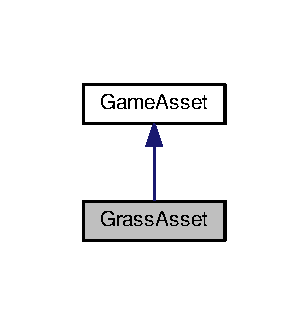
\includegraphics[width=148pt]{classGrassAsset__inherit__graph}
\end{center}
\end{figure}


Collaboration diagram for Grass\+Asset\+:\nopagebreak
\begin{figure}[H]
\begin{center}
\leavevmode
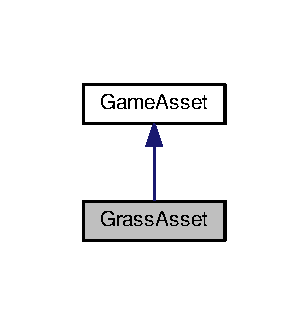
\includegraphics[width=148pt]{classGrassAsset__coll__graph}
\end{center}
\end{figure}
\subsection*{Public Member Functions}
\begin{DoxyCompactItemize}
\item 
\hyperlink{classGrassAsset_a961ec7133a9fc6f16a7347a122f95952}{Grass\+Asset} (G\+Lfloat x, G\+Lfloat y, G\+Lfloat z)
\item 
\hyperlink{classGrassAsset_a07e2206bacd2ec120f27f20e5df635b7}{$\sim$\+Grass\+Asset} ()
\item 
virtual void \hyperlink{classGrassAsset_a0178a72c5bf2f00bcc6a240b851f3a25}{Draw} (G\+Luint)
\item 
void \hyperlink{classGrassAsset_a06cf99092ea2217df1855e2d6375396b}{check\+Error} (std\+::string file, int line)
\end{DoxyCompactItemize}


\subsection{Constructor \& Destructor Documentation}
\hypertarget{classGrassAsset_a961ec7133a9fc6f16a7347a122f95952}{}\index{Grass\+Asset@{Grass\+Asset}!Grass\+Asset@{Grass\+Asset}}
\index{Grass\+Asset@{Grass\+Asset}!Grass\+Asset@{Grass\+Asset}}
\subsubsection[{Grass\+Asset(\+G\+Lfloat x, G\+Lfloat y, G\+Lfloat z)}]{\setlength{\rightskip}{0pt plus 5cm}Grass\+Asset\+::\+Grass\+Asset (
\begin{DoxyParamCaption}
\item[{G\+Lfloat}]{x, }
\item[{G\+Lfloat}]{y, }
\item[{G\+Lfloat}]{z}
\end{DoxyParamCaption}
)}\label{classGrassAsset_a961ec7133a9fc6f16a7347a122f95952}
Sets cordinates to a Grass/\+Pyramid with the center point 0.\+0 but moved to where the x, y, z variables calls them

Colour of Diamond Asset Green Uses R\+G\+B values
\begin{DoxyCode}
3                                                       \{
4 
5   \textcolor{comment}{// model coordinates, origin at centre.}
10 \textcolor{comment}{}  GLfloat vertex\_buffer [] \{
11       -0.01f + x  , 0.00f + y   ,-0.01f + z
12      , 0.01f + x  , 0.00f + y   ,-0.01f + z
13      ,-0.01f + x  , 0.00f + y   , 0.01f + z
14      , 0.01f + x  , 0.00f + y   , 0.01f + z
15      , 0.00f + x  , 0.60f + y   , 0.00f + z
16   \};
17   GLfloat vertex\_buffer\_length = \textcolor{keyword}{sizeof}(vertex\_buffer);
22   GLfloat colour\_buffer[] = \{
23 
24      0.000f, 1.000f, 0.000f,
25      0.000f, 1.000f, 0.000f,
26      0.000f, 1.000f, 0.000f,
27      0.000f, 1.000f, 0.000f,
28      0.000f, 1.000f, 0.000f
29   \};
30  colour\_buffer\_length = \textcolor{keyword}{sizeof}(colour\_buffer);
31   
32   GLuint element\_buffer []  \{
33       0, 4, 1   
34     , 1, 4, 3
35     , 2, 4, 3   
36     , 2, 4, 0
37     , 0, 2, 1
38     , 1, 2, 3
39   \};
40   element\_buffer\_length = \textcolor{keyword}{sizeof}(element\_buffer);
41 
42 
43 
44   \textcolor{comment}{// Transfer buffers to the GPU}
45 
46   \textcolor{comment}{// create buffer}
47   glGenBuffers(1, &vertex\_buffer\_token);
48   \textcolor{comment}{// immediately bind the buffer and transfer the data}
49   glBindBuffer(GL\_ARRAY\_BUFFER, vertex\_buffer\_token);
50   glBufferData(GL\_ARRAY\_BUFFER, vertex\_buffer\_length, vertex\_buffer, GL\_STATIC\_DRAW);
51 
52   \textcolor{comment}{// Binds the buffer and transfers the data}
53   glGenBuffers(1, &colour\_buffer\_token);
54   glBindBuffer(GL\_ARRAY\_BUFFER, colour\_buffer\_token);
55   glBufferData(GL\_ARRAY\_BUFFER, colour\_buffer\_length, colour\_buffer, GL\_STATIC\_DRAW);
56 
57 
58   glGenBuffers(1, &element\_buffer\_token);
59   glBindBuffer(GL\_ELEMENT\_ARRAY\_BUFFER, element\_buffer\_token);
60   glBufferData(GL\_ELEMENT\_ARRAY\_BUFFER, element\_buffer\_length, element\_buffer, GL\_STATIC\_DRAW);
61 \}
\end{DoxyCode}
\hypertarget{classGrassAsset_a07e2206bacd2ec120f27f20e5df635b7}{}\index{Grass\+Asset@{Grass\+Asset}!````~Grass\+Asset@{$\sim$\+Grass\+Asset}}
\index{````~Grass\+Asset@{$\sim$\+Grass\+Asset}!Grass\+Asset@{Grass\+Asset}}
\subsubsection[{$\sim$\+Grass\+Asset()}]{\setlength{\rightskip}{0pt plus 5cm}Grass\+Asset\+::$\sim$\+Grass\+Asset (
\begin{DoxyParamCaption}
{}
\end{DoxyParamCaption}
)}\label{classGrassAsset_a07e2206bacd2ec120f27f20e5df635b7}

\begin{DoxyCode}
63                         \{
64 \}
\end{DoxyCode}


\subsection{Member Function Documentation}
\hypertarget{classGrassAsset_a06cf99092ea2217df1855e2d6375396b}{}\index{Grass\+Asset@{Grass\+Asset}!check\+Error@{check\+Error}}
\index{check\+Error@{check\+Error}!Grass\+Asset@{Grass\+Asset}}
\subsubsection[{check\+Error(std\+::string file, int line)}]{\setlength{\rightskip}{0pt plus 5cm}void Grass\+Asset\+::check\+Error (
\begin{DoxyParamCaption}
\item[{std\+::string}]{file, }
\item[{int}]{line}
\end{DoxyParamCaption}
)}\label{classGrassAsset_a06cf99092ea2217df1855e2d6375396b}

\begin{DoxyCode}
73                                                     \{
74   GLenum gl\_error = glGetError();
75   \textcolor{keywordflow}{if}(GL\_NO\_ERROR != gl\_error) \{
76     std::cerr << \textcolor{stringliteral}{"GL error in "} << file << \textcolor{stringliteral}{" at line "} << line << \textcolor{stringliteral}{" error: "} << gl\_error << std::endl;
77     exit(-1);
78   \}
79 \}
\end{DoxyCode}
\hypertarget{classGrassAsset_a0178a72c5bf2f00bcc6a240b851f3a25}{}\index{Grass\+Asset@{Grass\+Asset}!Draw@{Draw}}
\index{Draw@{Draw}!Grass\+Asset@{Grass\+Asset}}
\subsubsection[{Draw(\+G\+Luint)}]{\setlength{\rightskip}{0pt plus 5cm}void Grass\+Asset\+::\+Draw (
\begin{DoxyParamCaption}
\item[{G\+Luint}]{program\+\_\+token}
\end{DoxyParamCaption}
)\hspace{0.3cm}{\ttfamily [virtual]}}\label{classGrassAsset_a0178a72c5bf2f00bcc6a240b851f3a25}
use the previously transferred buffer as the vertex array. This way we transfer the buffer once -- at construction -- not on every frame.

Uses the Previously transferred buffer as the color array. This way We transfer the buffer once -- at constuction -- not on every frame

Implements \hyperlink{classGameAsset_a961aa51ca0a9961fc584c0b5d5431300}{Game\+Asset}.


\begin{DoxyCode}
81                                           \{
82   \textcolor{keywordflow}{if}(!glIsProgram(program\_token)) \{
83     std::cerr << \textcolor{stringliteral}{"Drawing Grass with invalid program"} << std::endl;
84     \textcolor{keywordflow}{return};
85   \}
86   GLint validation\_ok;
87   glValidateProgram(program\_token);
88   glGetProgramiv(program\_token, GL\_VALIDATE\_STATUS, &validation\_ok);
89   \textcolor{keywordflow}{if}(!validation\_ok) \{
90     GLint maxLength = 0;
91     glGetProgramiv(program\_token, GL\_INFO\_LOG\_LENGTH, &maxLength);
92 
93     \textcolor{comment}{// The maxLength includes the NULL character}
94     std::vector<char> errorLog(maxLength);
95     glGetProgramInfoLog(program\_token, maxLength, &maxLength, &errorLog[0]);
96 
97     std::cerr << \textcolor{stringliteral}{"Invalid program "} << program\_token << \textcolor{stringliteral}{" with error code "} << validation\_ok << std::endl;
98     \textcolor{keywordflow}{for}(\textcolor{keyword}{auto} c: errorLog) \{
99       std::cerr << c;
100     \}
101     exit(-1);
102   \}
103 
104   GLuint position\_attrib = glGetAttribLocation(program\_token, \textcolor{stringliteral}{"position"});
105   \hyperlink{GrassAsset_8cc_a75f201b0e53e68726854997957322b8d}{checkGLError}();
106 
107   glUseProgram(program\_token);
108   \hyperlink{GrassAsset_8cc_a75f201b0e53e68726854997957322b8d}{checkGLError}();
113   glEnableVertexAttribArray(0);
114   glBindBuffer(GL\_ARRAY\_BUFFER, vertex\_buffer\_token);
115   glVertexAttribPointer(
116     position\_attrib,        \textcolor{comment}{/* attribute */}
117     3,        \textcolor{comment}{/* size */}
118     GL\_FLOAT,   \textcolor{comment}{/* type */}
119     GL\_FALSE,   \textcolor{comment}{/* normalized? */}
120     0,        \textcolor{comment}{/* stride */}
121     (\textcolor{keywordtype}{void}*)0    \textcolor{comment}{/* array buffer offset */}
122   );
123   glEnableVertexAttribArray(1);
124   \hyperlink{GrassAsset_8cc_a75f201b0e53e68726854997957322b8d}{checkGLError}();
129   glBindBuffer(GL\_ARRAY\_BUFFER, colour\_buffer\_token);
130   glVertexAttribPointer(
131     1,        \textcolor{comment}{/* attribute */}
132     3,        \textcolor{comment}{/* size */}
133     GL\_FLOAT,   \textcolor{comment}{/* type */}
134     GL\_FALSE,   \textcolor{comment}{/* normalized? */}
135     0,        \textcolor{comment}{/* stride */}
136     (\textcolor{keywordtype}{void}*)0    \textcolor{comment}{/* array buffer offset */}
137   );
138   \hyperlink{GrassAsset_8cc_a75f201b0e53e68726854997957322b8d}{checkGLError}();
139 
140   glBindBuffer(GL\_ELEMENT\_ARRAY\_BUFFER, element\_buffer\_token);
141   glDrawElements(
142     GL\_TRIANGLES,
143     element\_buffer\_length,
144     GL\_UNSIGNED\_INT,
145     (GLvoid*) 0
146   );
147   \hyperlink{GrassAsset_8cc_a75f201b0e53e68726854997957322b8d}{checkGLError}();
148 
149   glDisableVertexAttribArray(position\_attrib);
150 \}
\end{DoxyCode}


The documentation for this class was generated from the following files\+:\begin{DoxyCompactItemize}
\item 
src/\hyperlink{GrassAsset_8h}{Grass\+Asset.\+h}\item 
src/\hyperlink{GrassAsset_8cc}{Grass\+Asset.\+cc}\end{DoxyCompactItemize}

\hypertarget{classGroundAsset}{}\section{Ground\+Asset Class Reference}
\label{classGroundAsset}\index{Ground\+Asset@{Ground\+Asset}}


{\ttfamily \#include $<$Ground\+Asset.\+h$>$}



Inheritance diagram for Ground\+Asset\+:\nopagebreak
\begin{figure}[H]
\begin{center}
\leavevmode
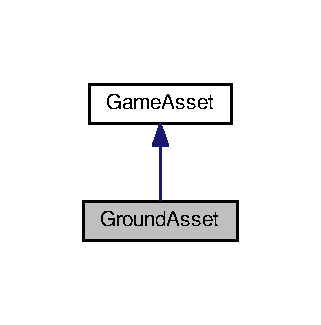
\includegraphics[width=154pt]{classGroundAsset__inherit__graph}
\end{center}
\end{figure}


Collaboration diagram for Ground\+Asset\+:\nopagebreak
\begin{figure}[H]
\begin{center}
\leavevmode
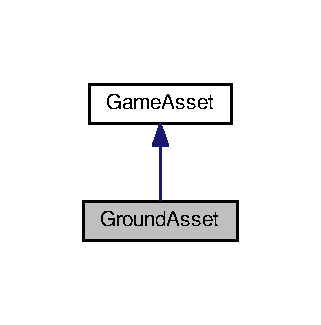
\includegraphics[width=154pt]{classGroundAsset__coll__graph}
\end{center}
\end{figure}
\subsection*{Public Member Functions}
\begin{DoxyCompactItemize}
\item 
\hyperlink{classGroundAsset_a4b927d07732cb30f8d5b35047bc2de22}{Ground\+Asset} (G\+Lfloat x, G\+Lfloat y, G\+Lfloat z)
\item 
\hyperlink{classGroundAsset_a8f607f3cabded6280c5a5eb2cbfa8c79}{$\sim$\+Ground\+Asset} ()
\item 
virtual void \hyperlink{classGroundAsset_a440f983638c7a7ccb6a39718444dfe95}{Draw} (G\+Luint)
\item 
void \hyperlink{classGroundAsset_a4fad6edd0d2f5aee6acc9a5a872aea96}{check\+Error} (std\+::string file, int line)
\end{DoxyCompactItemize}


\subsection{Constructor \& Destructor Documentation}
\hypertarget{classGroundAsset_a4b927d07732cb30f8d5b35047bc2de22}{}\index{Ground\+Asset@{Ground\+Asset}!Ground\+Asset@{Ground\+Asset}}
\index{Ground\+Asset@{Ground\+Asset}!Ground\+Asset@{Ground\+Asset}}
\subsubsection[{Ground\+Asset(\+G\+Lfloat x, G\+Lfloat y, G\+Lfloat z)}]{\setlength{\rightskip}{0pt plus 5cm}Ground\+Asset\+::\+Ground\+Asset (
\begin{DoxyParamCaption}
\item[{G\+Lfloat}]{x, }
\item[{G\+Lfloat}]{y, }
\item[{G\+Lfloat}]{z}
\end{DoxyParamCaption}
)}\label{classGroundAsset_a4b927d07732cb30f8d5b35047bc2de22}
model coordinates, origin at centre.

Sets cordinates to a Ground with the center point 0.\+0 but moved to where the x, y, z variables calls them

Colour of Diamond Asset Lawn Green Uses R\+G\+B values

Transfer buffers to the G\+P\+U

create buffer

immediately bind the buffer and transfer the data

Binds the buffer and transfers the data 
\begin{DoxyCode}
3                                                          \{
4   
6 
10   GLfloat vertex\_buffer [] \{
11       0.5f + x  , 0.5f + y  , -0.5f + z
12     , 0.5f + x  ,-0.5f + y  , -0.5f + z
13     ,-0.5f + x  , 0.5f + y  , -0.5f + z
14     ,-0.5f + x  ,-0.5f + y  , -0.5f + z
15     , 0.5f + x  , 0.5f + y  ,  0.5f + z
16     , 0.5f + x  ,-0.5f + y  ,  0.5f + z
17     ,-0.5f + x  , 0.5f + y  ,  0.5f + z
18     ,-0.5f + x  ,-0.5f + y  ,  0.5f + z
19   \};
20   GLfloat vertex\_buffer\_length = \textcolor{keyword}{sizeof}(vertex\_buffer);
25   GLfloat colour\_buffer[] = \{
26 
27      0.124f, 0.252f, 0.000f,
28      0.124f, 0.252f, 0.000f,
29      0.124f, 0.252f, 0.000f,
30      0.124f, 0.252f, 0.000f,
31      0.124f, 0.252f, 0.000f,
32      0.124f, 0.252f, 0.000f,
33      0.124f, 0.252f, 0.000f,
34      0.124f, 0.252f, 0.000f
35   \};
36   colour\_buffer\_length = \textcolor{keyword}{sizeof}(colour\_buffer);
37   
38   GLuint element\_buffer []  \{
39       0, 1, 2   
40     , 1, 3, 2
41     , 0, 4, 1   
42     , 1, 5, 4   
43     , 5, 7, 4   
44     , 7, 6, 4   
45     , 3, 7, 6   
46     , 2, 3, 6   
47     , 1, 5, 7   
48     , 1, 3, 7   
49     , 0, 4, 6   
50     , 0, 2, 6   
51   \};
52   element\_buffer\_length = \textcolor{keyword}{sizeof}(element\_buffer);
53 
54 
56 
58   glGenBuffers(1, &vertex\_buffer\_token);
60   glBindBuffer(GL\_ARRAY\_BUFFER, vertex\_buffer\_token);
61   glBufferData(GL\_ARRAY\_BUFFER, vertex\_buffer\_length, vertex\_buffer, GL\_STATIC\_DRAW);
62 
64   glGenBuffers(1, &colour\_buffer\_token);
65   glBindBuffer(GL\_ARRAY\_BUFFER, colour\_buffer\_token);
66   glBufferData(GL\_ARRAY\_BUFFER, colour\_buffer\_length, colour\_buffer, GL\_STATIC\_DRAW);
67 
68 
69   glGenBuffers(1, &element\_buffer\_token);
70   glBindBuffer(GL\_ELEMENT\_ARRAY\_BUFFER, element\_buffer\_token);
71   glBufferData(GL\_ELEMENT\_ARRAY\_BUFFER, element\_buffer\_length, element\_buffer, GL\_STATIC\_DRAW);
72 \}
\end{DoxyCode}
\hypertarget{classGroundAsset_a8f607f3cabded6280c5a5eb2cbfa8c79}{}\index{Ground\+Asset@{Ground\+Asset}!````~Ground\+Asset@{$\sim$\+Ground\+Asset}}
\index{````~Ground\+Asset@{$\sim$\+Ground\+Asset}!Ground\+Asset@{Ground\+Asset}}
\subsubsection[{$\sim$\+Ground\+Asset()}]{\setlength{\rightskip}{0pt plus 5cm}Ground\+Asset\+::$\sim$\+Ground\+Asset (
\begin{DoxyParamCaption}
{}
\end{DoxyParamCaption}
)}\label{classGroundAsset_a8f607f3cabded6280c5a5eb2cbfa8c79}

\begin{DoxyCode}
74                           \{
75 \}
\end{DoxyCode}


\subsection{Member Function Documentation}
\hypertarget{classGroundAsset_a4fad6edd0d2f5aee6acc9a5a872aea96}{}\index{Ground\+Asset@{Ground\+Asset}!check\+Error@{check\+Error}}
\index{check\+Error@{check\+Error}!Ground\+Asset@{Ground\+Asset}}
\subsubsection[{check\+Error(std\+::string file, int line)}]{\setlength{\rightskip}{0pt plus 5cm}void Ground\+Asset\+::check\+Error (
\begin{DoxyParamCaption}
\item[{std\+::string}]{file, }
\item[{int}]{line}
\end{DoxyParamCaption}
)}\label{classGroundAsset_a4fad6edd0d2f5aee6acc9a5a872aea96}

\begin{DoxyCode}
84                                                      \{
85   GLenum gl\_error = glGetError();
86   \textcolor{keywordflow}{if}(GL\_NO\_ERROR != gl\_error) \{
87     std::cerr << \textcolor{stringliteral}{"GL error in "} << file << \textcolor{stringliteral}{" at line "} << line << \textcolor{stringliteral}{" error: "} << gl\_error << std::endl;
88     exit(-1);
89   \}
90 \}
\end{DoxyCode}
\hypertarget{classGroundAsset_a440f983638c7a7ccb6a39718444dfe95}{}\index{Ground\+Asset@{Ground\+Asset}!Draw@{Draw}}
\index{Draw@{Draw}!Ground\+Asset@{Ground\+Asset}}
\subsubsection[{Draw(\+G\+Luint)}]{\setlength{\rightskip}{0pt plus 5cm}void Ground\+Asset\+::\+Draw (
\begin{DoxyParamCaption}
\item[{G\+Luint}]{program\+\_\+token}
\end{DoxyParamCaption}
)\hspace{0.3cm}{\ttfamily [virtual]}}\label{classGroundAsset_a440f983638c7a7ccb6a39718444dfe95}
The max\+Length includes the N\+U\+L\+L character

use the previously transferred buffer as the vertex array. This way we transfer the buffer once -- at construction -- not on every frame.

attribute

size

type

normalized?

stride

array buffer offset

Uses the Previously transferred buffer as the color array. This way We transfer the buffer once -- at constuction -- not on every frame

attribute

size

type

normalized?

stride

array buffer offset 

Implements \hyperlink{classGameAsset_a961aa51ca0a9961fc584c0b5d5431300}{Game\+Asset}.


\begin{DoxyCode}
93                                            \{
94   \textcolor{keywordflow}{if}(!glIsProgram(program\_token)) \{
95     std::cerr << \textcolor{stringliteral}{"Drawing Cube with invalid program"} << std::endl;
96     \textcolor{keywordflow}{return};
97   \}
98   GLint validation\_ok;
99   glValidateProgram(program\_token);
100   glGetProgramiv(program\_token, GL\_VALIDATE\_STATUS, &validation\_ok);
101   \textcolor{keywordflow}{if}(!validation\_ok) \{
102     GLint maxLength = 0;
103     glGetProgramiv(program\_token, GL\_INFO\_LOG\_LENGTH, &maxLength);
104 
106     std::vector<char> errorLog(maxLength);
107     glGetProgramInfoLog(program\_token, maxLength, &maxLength, &errorLog[0]);
108 
109     std::cerr << \textcolor{stringliteral}{"Invalid program "} << program\_token << \textcolor{stringliteral}{" with error code "} << validation\_ok << std::endl;
110     \textcolor{keywordflow}{for}(\textcolor{keyword}{auto} c: errorLog) \{
111       std::cerr << c;
112     \}
113     exit(-1);
114   \}
115 
116   GLuint position\_attrib = glGetAttribLocation(program\_token, \textcolor{stringliteral}{"position"});
117   \hyperlink{GroundAsset_8cc_a75f201b0e53e68726854997957322b8d}{checkGLError}();
118 
119   glUseProgram(program\_token);
120   \hyperlink{GroundAsset_8cc_a75f201b0e53e68726854997957322b8d}{checkGLError}();
121 
125   glEnableVertexAttribArray(0);
126   glBindBuffer(GL\_ARRAY\_BUFFER, vertex\_buffer\_token);
127   glVertexAttribPointer(
128     position\_attrib,        
129     3,        
130     GL\_FLOAT,   
131     GL\_FALSE,   
132     0,        
133     (\textcolor{keywordtype}{void}*)0    
134   );
135   glEnableVertexAttribArray(1);
136   \hyperlink{GroundAsset_8cc_a75f201b0e53e68726854997957322b8d}{checkGLError}();
141   glBindBuffer(GL\_ARRAY\_BUFFER, colour\_buffer\_token);
142   glVertexAttribPointer(
143     1,        
144     3,        
145     GL\_FLOAT,   
146     GL\_FALSE,   
147     0,        
148     (\textcolor{keywordtype}{void}*)0    
149   );
150   \hyperlink{GroundAsset_8cc_a75f201b0e53e68726854997957322b8d}{checkGLError}();
151 
152   glBindBuffer(GL\_ELEMENT\_ARRAY\_BUFFER, element\_buffer\_token);
153   glDrawElements(
154     GL\_TRIANGLES,
155     element\_buffer\_length,
156     GL\_UNSIGNED\_INT,
157     (GLvoid*) 0
158   );
159   \hyperlink{GroundAsset_8cc_a75f201b0e53e68726854997957322b8d}{checkGLError}();
160 
161   glDisableVertexAttribArray(position\_attrib);
162 \}
\end{DoxyCode}


The documentation for this class was generated from the following files\+:\begin{DoxyCompactItemize}
\item 
src/\hyperlink{GroundAsset_8h}{Ground\+Asset.\+h}\item 
src/\hyperlink{GroundAsset_8cc}{Ground\+Asset.\+cc}\end{DoxyCompactItemize}

\hypertarget{classLeavesAsset}{}\section{Leaves\+Asset Class Reference}
\label{classLeavesAsset}\index{Leaves\+Asset@{Leaves\+Asset}}


{\ttfamily \#include $<$Leaves\+Asset.\+h$>$}



Inheritance diagram for Leaves\+Asset\+:\nopagebreak
\begin{figure}[H]
\begin{center}
\leavevmode
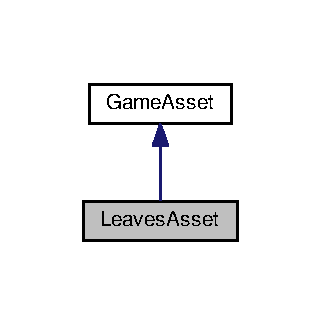
\includegraphics[width=154pt]{classLeavesAsset__inherit__graph}
\end{center}
\end{figure}


Collaboration diagram for Leaves\+Asset\+:\nopagebreak
\begin{figure}[H]
\begin{center}
\leavevmode
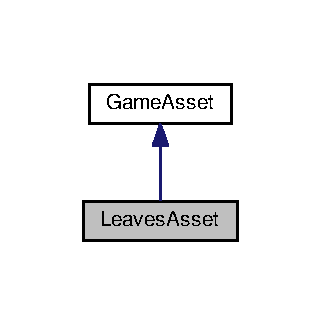
\includegraphics[width=154pt]{classLeavesAsset__coll__graph}
\end{center}
\end{figure}
\subsection*{Public Member Functions}
\begin{DoxyCompactItemize}
\item 
\hyperlink{classLeavesAsset_a1fb1212e5399f16071f0be7ff42cc344}{Leaves\+Asset} (G\+Lfloat x, G\+Lfloat y, G\+Lfloat z)
\item 
\hyperlink{classLeavesAsset_ae98d43a307f4c75cc8a661f0b36a213a}{$\sim$\+Leaves\+Asset} ()
\item 
virtual void \hyperlink{classLeavesAsset_a807fd196b83e5adb131d489ef6645742}{Draw} (G\+Luint)
\end{DoxyCompactItemize}


\subsection{Constructor \& Destructor Documentation}
\hypertarget{classLeavesAsset_a1fb1212e5399f16071f0be7ff42cc344}{}\index{Leaves\+Asset@{Leaves\+Asset}!Leaves\+Asset@{Leaves\+Asset}}
\index{Leaves\+Asset@{Leaves\+Asset}!Leaves\+Asset@{Leaves\+Asset}}
\subsubsection[{Leaves\+Asset(\+G\+Lfloat x, G\+Lfloat y, G\+Lfloat z)}]{\setlength{\rightskip}{0pt plus 5cm}Leaves\+Asset\+::\+Leaves\+Asset (
\begin{DoxyParamCaption}
\item[{G\+Lfloat}]{x, }
\item[{G\+Lfloat}]{y, }
\item[{G\+Lfloat}]{z}
\end{DoxyParamCaption}
)}\label{classLeavesAsset_a1fb1212e5399f16071f0be7ff42cc344}
model coordinates, origin at centre. Sets cordinates to a Cube with the center point 0.\+0 but moved to where the x, y, z variables calls them from the gameworld class through the G\+Lfloat x,y,z variables.

Color Buffer. Colour of Cube Camerone Green \& Lawn Green Uses R\+G\+B values to set the colour.
\begin{DoxyCode}
3                                                         \{
4 
11   GLfloat vertex\_buffer [] \{
12       0.5f + x  , 0.5f + y  , -0.5f + z
13     , 0.5f + x  ,-0.5f + y  , -0.5f + z
14     ,-0.5f + x  , 0.5f + y  , -0.5f + z
15     ,-0.5f + x  ,-0.5f + y  , -0.5f + z
16     , 0.5f + x  , 0.5f + y  ,  0.5f + z
17     , 0.5f + x  ,-0.5f + y  ,  0.5f + z
18     ,-0.5f + x  , 0.5f + y  ,  0.5f + z
19     ,-0.5f + x  ,-0.5f + y  ,  0.5f + z
20   \};
21   GLfloat vertex\_buffer\_length = \textcolor{keyword}{sizeof}(vertex\_buffer);
27   GLfloat colour\_buffer[] = \{
28 
29      0.000f, 0.090f, 0.004f, 
30      0.058f, 0.095f, 0.011f,
31      0.000f, 0.090f, 0.004f,
32      0.058f, 0.095f, 0.011f,
33      0.000f, 0.090f, 0.004f,
34      0.058f, 0.095f, 0.011f,
35      0.000f, 0.090f, 0.004f,
36      0.058f, 0.095f, 0.011f,
37 
38   \};
39  colour\_buffer\_length = \textcolor{keyword}{sizeof}(colour\_buffer);
40   
41   GLuint element\_buffer []  \{
42       0, 1, 2   
43     , 1, 3, 2
44     , 0, 4, 1   
45     , 1, 5, 4   
46     , 5, 7, 4   
47     , 7, 6, 4   
48     , 3, 7, 6   
49     , 2, 3, 6   
50     , 1, 5, 7   
51     , 1, 3, 7   
52     , 0, 4, 6   
53     , 0, 2, 6   
54   \};
55   element\_buffer\_length = \textcolor{keyword}{sizeof}(element\_buffer);
56 
57 
58 
59   \textcolor{comment}{// Transfer buffers to the GPU}
60 
61 
62   \textcolor{comment}{// create buffer}
63   glGenBuffers(1, &vertex\_buffer\_token);
64   \textcolor{comment}{// immediately bind the buffer and transfer the data}
65   glBindBuffer(GL\_ARRAY\_BUFFER, vertex\_buffer\_token);
66   glBufferData(GL\_ARRAY\_BUFFER, vertex\_buffer\_length, vertex\_buffer, GL\_STATIC\_DRAW);
67 
68   \textcolor{comment}{// Binds the buffer and transfers the data}
69   glGenBuffers(1, &colour\_buffer\_token);
70   glBindBuffer(GL\_ARRAY\_BUFFER, colour\_buffer\_token);
71   glBufferData(GL\_ARRAY\_BUFFER, colour\_buffer\_length, colour\_buffer, GL\_STATIC\_DRAW);
72 
73 
74   glGenBuffers(1, &element\_buffer\_token);
75   glBindBuffer(GL\_ELEMENT\_ARRAY\_BUFFER, element\_buffer\_token);
76   glBufferData(GL\_ELEMENT\_ARRAY\_BUFFER, element\_buffer\_length, element\_buffer, GL\_STATIC\_DRAW);
77 \}
\end{DoxyCode}
\hypertarget{classLeavesAsset_ae98d43a307f4c75cc8a661f0b36a213a}{}\index{Leaves\+Asset@{Leaves\+Asset}!````~Leaves\+Asset@{$\sim$\+Leaves\+Asset}}
\index{````~Leaves\+Asset@{$\sim$\+Leaves\+Asset}!Leaves\+Asset@{Leaves\+Asset}}
\subsubsection[{$\sim$\+Leaves\+Asset()}]{\setlength{\rightskip}{0pt plus 5cm}Leaves\+Asset\+::$\sim$\+Leaves\+Asset (
\begin{DoxyParamCaption}
{}
\end{DoxyParamCaption}
)}\label{classLeavesAsset_ae98d43a307f4c75cc8a661f0b36a213a}

\begin{DoxyCode}
79                           \{
80 \}
\end{DoxyCode}


\subsection{Member Function Documentation}
\hypertarget{classLeavesAsset_a807fd196b83e5adb131d489ef6645742}{}\index{Leaves\+Asset@{Leaves\+Asset}!Draw@{Draw}}
\index{Draw@{Draw}!Leaves\+Asset@{Leaves\+Asset}}
\subsubsection[{Draw(\+G\+Luint)}]{\setlength{\rightskip}{0pt plus 5cm}void Leaves\+Asset\+::\+Draw (
\begin{DoxyParamCaption}
\item[{G\+Luint}]{program\+\_\+token}
\end{DoxyParamCaption}
)\hspace{0.3cm}{\ttfamily [virtual]}}\label{classLeavesAsset_a807fd196b83e5adb131d489ef6645742}
use the previously transferred buffer as the vertex array. This way we transfer the buffer once -- at construction -- not on every frame.

Uses the Previously transferred buffer as the color array. This way We transfer the buffer once -- at constuction -- not on every frame

Implements \hyperlink{classGameAsset_a961aa51ca0a9961fc584c0b5d5431300}{Game\+Asset}.


\begin{DoxyCode}
97                                            \{
98   \textcolor{keywordflow}{if}(!glIsProgram(program\_token)) \{
99     std::cerr << \textcolor{stringliteral}{"Drawing Diamon with invalid program"} << std::endl;
100     \textcolor{keywordflow}{return};
101   \}
102   GLint validation\_ok;
103   glValidateProgram(program\_token);
104   glGetProgramiv(program\_token, GL\_VALIDATE\_STATUS, &validation\_ok);
105   \textcolor{keywordflow}{if}(!validation\_ok) \{
106     GLint maxLength = 0;
107     glGetProgramiv(program\_token, GL\_INFO\_LOG\_LENGTH, &maxLength);
108 
109     \textcolor{comment}{// The maxLength includes the NULL character}
110     std::vector<char> errorLog(maxLength);
111     glGetProgramInfoLog(program\_token, maxLength, &maxLength, &errorLog[0]);
112 
113     std::cerr << \textcolor{stringliteral}{"Invalid program "} << program\_token << \textcolor{stringliteral}{" with error code "} << validation\_ok << std::endl;
114     \textcolor{keywordflow}{for}(\textcolor{keyword}{auto} c: errorLog) \{
115       std::cerr << c;
116     \}
117     exit(-1);
118   \}
119 
120   GLuint position\_attrib = glGetAttribLocation(program\_token, \textcolor{stringliteral}{"position"});
121   \hyperlink{LeavesAsset_8cc_a75f201b0e53e68726854997957322b8d}{checkGLError}();
122 
123   glUseProgram(program\_token);
124   \hyperlink{LeavesAsset_8cc_a75f201b0e53e68726854997957322b8d}{checkGLError}();
129   glEnableVertexAttribArray(0);
130   glBindBuffer(GL\_ARRAY\_BUFFER, vertex\_buffer\_token);
131   glVertexAttribPointer(
132     position\_attrib,        \textcolor{comment}{/* attribute */}
133     3,        \textcolor{comment}{/* size */}
134     GL\_FLOAT,   \textcolor{comment}{/* type */}
135     GL\_FALSE,   \textcolor{comment}{/* normalized? */}
136     0,        \textcolor{comment}{/* stride */}
137     (\textcolor{keywordtype}{void}*)0    \textcolor{comment}{/* array buffer offset */}
138   );
139   glEnableVertexAttribArray(1);
140   \hyperlink{LeavesAsset_8cc_a75f201b0e53e68726854997957322b8d}{checkGLError}();
145   glBindBuffer(GL\_ARRAY\_BUFFER, colour\_buffer\_token);
146   glVertexAttribPointer(
147     1,        \textcolor{comment}{/* attribute */}
148     3,        \textcolor{comment}{/* size */}
149     GL\_FLOAT,   \textcolor{comment}{/* type */}
150     GL\_FALSE,   \textcolor{comment}{/* normalized? */}
151     0,        \textcolor{comment}{/* stride */}
152     (\textcolor{keywordtype}{void}*)0    \textcolor{comment}{/* array buffer offset */}
153   );
154   \hyperlink{LeavesAsset_8cc_a75f201b0e53e68726854997957322b8d}{checkGLError}();
155 
156   glBindBuffer(GL\_ELEMENT\_ARRAY\_BUFFER, element\_buffer\_token);
157   glDrawElements(
158     GL\_TRIANGLES,
159     element\_buffer\_length,
160     GL\_UNSIGNED\_INT,
161     (GLvoid*) 0
162   );
163   \hyperlink{LeavesAsset_8cc_a75f201b0e53e68726854997957322b8d}{checkGLError}();
164 
165   glDisableVertexAttribArray(position\_attrib);
166 \}
\end{DoxyCode}


The documentation for this class was generated from the following files\+:\begin{DoxyCompactItemize}
\item 
src/\hyperlink{LeavesAsset_8h}{Leaves\+Asset.\+h}\item 
src/\hyperlink{LeavesAsset_8cc}{Leaves\+Asset.\+cc}\end{DoxyCompactItemize}

\hypertarget{classPyramidAsset}{}\section{Pyramid\+Asset Class Reference}
\label{classPyramidAsset}\index{Pyramid\+Asset@{Pyramid\+Asset}}


{\ttfamily \#include $<$Pyramid\+Asset.\+h$>$}



Inheritance diagram for Pyramid\+Asset\+:\nopagebreak
\begin{figure}[H]
\begin{center}
\leavevmode
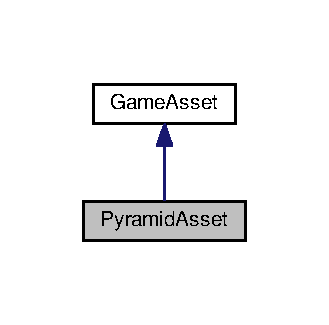
\includegraphics[width=158pt]{classPyramidAsset__inherit__graph}
\end{center}
\end{figure}


Collaboration diagram for Pyramid\+Asset\+:\nopagebreak
\begin{figure}[H]
\begin{center}
\leavevmode
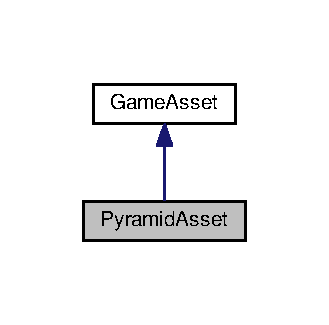
\includegraphics[width=158pt]{classPyramidAsset__coll__graph}
\end{center}
\end{figure}
\subsection*{Public Member Functions}
\begin{DoxyCompactItemize}
\item 
\hyperlink{classPyramidAsset_a3f7c6fd658ed0d3e276d7fe6c1de95d1}{Pyramid\+Asset} (G\+Lfloat x, G\+Lfloat y, G\+Lfloat z)
\item 
\hyperlink{classPyramidAsset_afb388a196f43a3808b2d4f6fdb89ee84}{$\sim$\+Pyramid\+Asset} ()
\item 
virtual void \hyperlink{classPyramidAsset_aaea45da4956d79ec9ab96e9d0ccef3fe}{Draw} (G\+Luint)
\item 
void \hyperlink{classPyramidAsset_a34350044042e0098446dc9e0a260cb70}{check\+Error} (std\+::string file, int line)
\end{DoxyCompactItemize}


\subsection{Constructor \& Destructor Documentation}
\hypertarget{classPyramidAsset_a3f7c6fd658ed0d3e276d7fe6c1de95d1}{}\index{Pyramid\+Asset@{Pyramid\+Asset}!Pyramid\+Asset@{Pyramid\+Asset}}
\index{Pyramid\+Asset@{Pyramid\+Asset}!Pyramid\+Asset@{Pyramid\+Asset}}
\subsubsection[{Pyramid\+Asset(\+G\+Lfloat x, G\+Lfloat y, G\+Lfloat z)}]{\setlength{\rightskip}{0pt plus 5cm}Pyramid\+Asset\+::\+Pyramid\+Asset (
\begin{DoxyParamCaption}
\item[{G\+Lfloat}]{x, }
\item[{G\+Lfloat}]{y, }
\item[{G\+Lfloat}]{z}
\end{DoxyParamCaption}
)}\label{classPyramidAsset_a3f7c6fd658ed0d3e276d7fe6c1de95d1}
Sets cordinates to a Pyramid with the center point 0.\+0 but moved to where the x, y, z variables calls them

Colour of Diamond Asset Red, Green \& Blue Uses R\+G\+B values
\begin{DoxyCode}
3                                                           \{
4 
5   \textcolor{comment}{// model coordinates, origin at centre.}
10 \textcolor{comment}{}  GLfloat vertex\_buffer [] \{
11       -0.5f + x  , 0.0f + y   ,-0.5f + z
12      , 0.5f + x  , 0.0f + y   ,-0.5f + z
13      ,-0.5f + x  , 0.0f + y   , 0.5f + z
14      , 0.5f + x  , 0.0f + y   , 0.5f + z
15      , 0.0f + x  , 1.0f + y   , 0.0f + z
16   \};
17   GLfloat vertex\_buffer\_length = \textcolor{keyword}{sizeof}(vertex\_buffer);
22   GLfloat colour\_buffer[] = \{
23 
24      1.000f, 0.000f, 0.000f,
25      0.000f, 1.000f, 0.000f,
26      0.000f, 0.000f, 1.000f,
27      1.000f, 0.000f, 0.000f,
28      0.000f, 1.000f, 0.000f,
29      0.000f, 0.000f, 1.000f,
30      1.000f, 0.000f, 0.000f,
31      0.000f, 1.000f, 0.000f,
32      0.000f, 0.000f, 1.000f
33   \};
34  colour\_buffer\_length = \textcolor{keyword}{sizeof}(colour\_buffer);
35   
36   GLuint element\_buffer []  \{
37       0, 4, 1   
38     , 1, 4, 3
39     , 2, 4, 3   
40     , 2, 4, 0
41     , 0, 2, 1
42     , 1, 2, 3
43   \};
44   element\_buffer\_length = \textcolor{keyword}{sizeof}(element\_buffer);
45 
46 
47 
48   \textcolor{comment}{// Transfer buffers to the GPU}
49 
50   \textcolor{comment}{// create buffer}
51   glGenBuffers(1, &vertex\_buffer\_token);
52   \textcolor{comment}{// immediately bind the buffer and transfer the data}
53   glBindBuffer(GL\_ARRAY\_BUFFER, vertex\_buffer\_token);
54   glBufferData(GL\_ARRAY\_BUFFER, vertex\_buffer\_length, vertex\_buffer, GL\_STATIC\_DRAW);
55 
56   \textcolor{comment}{// Binds the buffer and transfers the data}
57   glGenBuffers(1, &colour\_buffer\_token);
58   glBindBuffer(GL\_ARRAY\_BUFFER, colour\_buffer\_token);
59   glBufferData(GL\_ARRAY\_BUFFER, colour\_buffer\_length, colour\_buffer, GL\_STATIC\_DRAW);
60 
61 
62   glGenBuffers(1, &element\_buffer\_token);
63   glBindBuffer(GL\_ELEMENT\_ARRAY\_BUFFER, element\_buffer\_token);
64   glBufferData(GL\_ELEMENT\_ARRAY\_BUFFER, element\_buffer\_length, element\_buffer, GL\_STATIC\_DRAW);
65 \}
\end{DoxyCode}
\hypertarget{classPyramidAsset_afb388a196f43a3808b2d4f6fdb89ee84}{}\index{Pyramid\+Asset@{Pyramid\+Asset}!````~Pyramid\+Asset@{$\sim$\+Pyramid\+Asset}}
\index{````~Pyramid\+Asset@{$\sim$\+Pyramid\+Asset}!Pyramid\+Asset@{Pyramid\+Asset}}
\subsubsection[{$\sim$\+Pyramid\+Asset()}]{\setlength{\rightskip}{0pt plus 5cm}Pyramid\+Asset\+::$\sim$\+Pyramid\+Asset (
\begin{DoxyParamCaption}
{}
\end{DoxyParamCaption}
)}\label{classPyramidAsset_afb388a196f43a3808b2d4f6fdb89ee84}

\begin{DoxyCode}
67                             \{
68 \}
\end{DoxyCode}


\subsection{Member Function Documentation}
\hypertarget{classPyramidAsset_a34350044042e0098446dc9e0a260cb70}{}\index{Pyramid\+Asset@{Pyramid\+Asset}!check\+Error@{check\+Error}}
\index{check\+Error@{check\+Error}!Pyramid\+Asset@{Pyramid\+Asset}}
\subsubsection[{check\+Error(std\+::string file, int line)}]{\setlength{\rightskip}{0pt plus 5cm}void Pyramid\+Asset\+::check\+Error (
\begin{DoxyParamCaption}
\item[{std\+::string}]{file, }
\item[{int}]{line}
\end{DoxyParamCaption}
)}\label{classPyramidAsset_a34350044042e0098446dc9e0a260cb70}

\begin{DoxyCode}
77                                                       \{
78   GLenum gl\_error = glGetError();
79   \textcolor{keywordflow}{if}(GL\_NO\_ERROR != gl\_error) \{
80     std::cerr << \textcolor{stringliteral}{"GL error in "} << file << \textcolor{stringliteral}{" at line "} << line << \textcolor{stringliteral}{" error: "} << gl\_error << std::endl;
81     exit(-1);
82   \}
83 \}
\end{DoxyCode}
\hypertarget{classPyramidAsset_aaea45da4956d79ec9ab96e9d0ccef3fe}{}\index{Pyramid\+Asset@{Pyramid\+Asset}!Draw@{Draw}}
\index{Draw@{Draw}!Pyramid\+Asset@{Pyramid\+Asset}}
\subsubsection[{Draw(\+G\+Luint)}]{\setlength{\rightskip}{0pt plus 5cm}void Pyramid\+Asset\+::\+Draw (
\begin{DoxyParamCaption}
\item[{G\+Luint}]{program\+\_\+token}
\end{DoxyParamCaption}
)\hspace{0.3cm}{\ttfamily [virtual]}}\label{classPyramidAsset_aaea45da4956d79ec9ab96e9d0ccef3fe}
use the previously transferred buffer as the vertex array. This way we transfer the buffer once -- at construction -- not on every frame.

Uses the Previously transferred buffer as the color array. This way We transfer the buffer once -- at constuction -- not on every frame

Implements \hyperlink{classGameAsset_a961aa51ca0a9961fc584c0b5d5431300}{Game\+Asset}.


\begin{DoxyCode}
85                                             \{
86   \textcolor{keywordflow}{if}(!glIsProgram(program\_token)) \{
87     std::cerr << \textcolor{stringliteral}{"Drawing Pyramid with invalid program"} << std::endl;
88     \textcolor{keywordflow}{return};
89   \}
90   GLint validation\_ok;
91   glValidateProgram(program\_token);
92   glGetProgramiv(program\_token, GL\_VALIDATE\_STATUS, &validation\_ok);
93   \textcolor{keywordflow}{if}(!validation\_ok) \{
94     GLint maxLength = 0;
95     glGetProgramiv(program\_token, GL\_INFO\_LOG\_LENGTH, &maxLength);
96 
97     \textcolor{comment}{// The maxLength includes the NULL character}
98     std::vector<char> errorLog(maxLength);
99     glGetProgramInfoLog(program\_token, maxLength, &maxLength, &errorLog[0]);
100 
101     std::cerr << \textcolor{stringliteral}{"Invalid program "} << program\_token << \textcolor{stringliteral}{" with error code "} << validation\_ok << std::endl;
102     \textcolor{keywordflow}{for}(\textcolor{keyword}{auto} c: errorLog) \{
103       std::cerr << c;
104     \}
105     exit(-1);
106   \}
107 
108   GLuint position\_attrib = glGetAttribLocation(program\_token, \textcolor{stringliteral}{"position"});
109   \hyperlink{PyramidAsset_8cc_a75f201b0e53e68726854997957322b8d}{checkGLError}();
110 
111   glUseProgram(program\_token);
112   \hyperlink{PyramidAsset_8cc_a75f201b0e53e68726854997957322b8d}{checkGLError}();
113 
118   glEnableVertexAttribArray(0);
119   glBindBuffer(GL\_ARRAY\_BUFFER, vertex\_buffer\_token);
120   glVertexAttribPointer(
121     position\_attrib,        \textcolor{comment}{/* attribute */}
122     3,        \textcolor{comment}{/* size */}
123     GL\_FLOAT,   \textcolor{comment}{/* type */}
124     GL\_FALSE,   \textcolor{comment}{/* normalized? */}
125     0,        \textcolor{comment}{/* stride */}
126     (\textcolor{keywordtype}{void}*)0    \textcolor{comment}{/* array buffer offset */}
127   );
128   glEnableVertexAttribArray(1);
129   \hyperlink{PyramidAsset_8cc_a75f201b0e53e68726854997957322b8d}{checkGLError}();
134   glBindBuffer(GL\_ARRAY\_BUFFER, colour\_buffer\_token);
135   glVertexAttribPointer(
136     1,        \textcolor{comment}{/* attribute */}
137     3,        \textcolor{comment}{/* size */}
138     GL\_FLOAT,   \textcolor{comment}{/* type */}
139     GL\_FALSE,   \textcolor{comment}{/* normalized? */}
140     0,        \textcolor{comment}{/* stride */}
141     (\textcolor{keywordtype}{void}*)0    \textcolor{comment}{/* array buffer offset */}
142   );
143   \hyperlink{PyramidAsset_8cc_a75f201b0e53e68726854997957322b8d}{checkGLError}();
144 
145   glBindBuffer(GL\_ELEMENT\_ARRAY\_BUFFER, element\_buffer\_token);
146   glDrawElements(
147     GL\_TRIANGLES,
148     element\_buffer\_length,
149     GL\_UNSIGNED\_INT,
150     (GLvoid*) 0
151   );
152   \hyperlink{PyramidAsset_8cc_a75f201b0e53e68726854997957322b8d}{checkGLError}();
153 
154   glDisableVertexAttribArray(position\_attrib);
155 \}
\end{DoxyCode}


The documentation for this class was generated from the following files\+:\begin{DoxyCompactItemize}
\item 
src/\hyperlink{PyramidAsset_8h}{Pyramid\+Asset.\+h}\item 
src/\hyperlink{PyramidAsset_8cc}{Pyramid\+Asset.\+cc}\end{DoxyCompactItemize}

\hypertarget{structSDLWindowDeleter}{}\section{S\+D\+L\+Window\+Deleter Struct Reference}
\label{structSDLWindowDeleter}\index{S\+D\+L\+Window\+Deleter@{S\+D\+L\+Window\+Deleter}}
\subsection*{Public Member Functions}
\begin{DoxyCompactItemize}
\item 
void \hyperlink{structSDLWindowDeleter_a2aedcc99c3756ae090c38badabeb10b1}{operator()} (S\+D\+L\+\_\+\+Window $\ast$window)
\end{DoxyCompactItemize}


\subsection{Member Function Documentation}
\hypertarget{structSDLWindowDeleter_a2aedcc99c3756ae090c38badabeb10b1}{}\index{S\+D\+L\+Window\+Deleter@{S\+D\+L\+Window\+Deleter}!operator()@{operator()}}
\index{operator()@{operator()}!S\+D\+L\+Window\+Deleter@{S\+D\+L\+Window\+Deleter}}
\subsubsection[{operator()(\+S\+D\+L\+\_\+\+Window $\ast$window)}]{\setlength{\rightskip}{0pt plus 5cm}void S\+D\+L\+Window\+Deleter\+::operator() (
\begin{DoxyParamCaption}
\item[{S\+D\+L\+\_\+\+Window $\ast$}]{window}
\end{DoxyParamCaption}
)\hspace{0.3cm}{\ttfamily [inline]}}\label{structSDLWindowDeleter_a2aedcc99c3756ae090c38badabeb10b1}

\begin{DoxyCode}
34                                              \{
35     SDL\_DestroyWindow(window);
36   \}
\end{DoxyCode}


The documentation for this struct was generated from the following file\+:\begin{DoxyCompactItemize}
\item 
src/\hyperlink{main_8cc}{main.\+cc}\end{DoxyCompactItemize}

\chapter{File Documentation}
\hypertarget{config_8h}{}\section{config.\+h File Reference}
\label{config_8h}\index{config.\+h@{config.\+h}}
\subsection*{Macros}
\begin{DoxyCompactItemize}
\item 
\#define \hyperlink{config_8h_a1644f282a4f84575a270f96b98d4f3c6}{H\+A\+V\+E\+\_\+\+B\+O\+O\+S\+T}~1
\item 
\#define \hyperlink{config_8h_ad428c9f5d2a48876c1eabd050fac47d2}{H\+A\+V\+E\+\_\+\+B\+O\+O\+S\+T\+\_\+\+P\+R\+O\+G\+R\+A\+M\+\_\+\+O\+P\+T\+I\+O\+N\+S\+\_\+\+H\+P\+P}~1
\item 
\#define \hyperlink{config_8h_a0ee1617ff2f6885ef384a3dd46f9b9d7}{H\+A\+V\+E\+\_\+\+D\+L\+F\+C\+N\+\_\+\+H}~1
\item 
\#define \hyperlink{config_8h_ab90a030ff2790ebdc176660a6dd2a478}{H\+A\+V\+E\+\_\+\+I\+N\+T\+T\+Y\+P\+E\+S\+\_\+\+H}~1
\item 
\#define \hyperlink{config_8h_ae93a78f9d076138897af441c9f86f285}{H\+A\+V\+E\+\_\+\+M\+E\+M\+O\+R\+Y\+\_\+\+H}~1
\item 
\#define \hyperlink{config_8h_ab6cd6d1c63c1e26ea2d4537b77148354}{H\+A\+V\+E\+\_\+\+S\+T\+D\+I\+N\+T\+\_\+\+H}~1
\item 
\#define \hyperlink{config_8h_a9e0e434ec1a6ddbd97db12b5a32905e0}{H\+A\+V\+E\+\_\+\+S\+T\+D\+L\+I\+B\+\_\+\+H}~1
\item 
\#define \hyperlink{config_8h_a405d10d46190bcb0320524c54eafc850}{H\+A\+V\+E\+\_\+\+S\+T\+R\+I\+N\+G\+S\+\_\+\+H}~1
\item 
\#define \hyperlink{config_8h_ad4c234dd1625255dc626a15886306e7d}{H\+A\+V\+E\+\_\+\+S\+T\+R\+I\+N\+G\+\_\+\+H}~1
\item 
\#define \hyperlink{config_8h_ace156430ba007d19b4348a950d0c692b}{H\+A\+V\+E\+\_\+\+S\+Y\+S\+\_\+\+S\+T\+A\+T\+\_\+\+H}~1
\item 
\#define \hyperlink{config_8h_a69dc70bea5d1f8bd2be9740e974fa666}{H\+A\+V\+E\+\_\+\+S\+Y\+S\+\_\+\+T\+Y\+P\+E\+S\+\_\+\+H}~1
\item 
\#define \hyperlink{config_8h_a219b06937831d0da94d801ab13987639}{H\+A\+V\+E\+\_\+\+U\+N\+I\+S\+T\+D\+\_\+\+H}~1
\item 
\#define \hyperlink{config_8h_ac2d5925d76379847dd9fc4747b061659}{L\+T\+\_\+\+O\+B\+J\+D\+I\+R}~\char`\"{}.libs/\char`\"{}
\item 
\#define \hyperlink{config_8h_aca8570fb706c81df371b7f9bc454ae03}{P\+A\+C\+K\+A\+G\+E}~\char`\"{}shaderexamples\char`\"{}
\item 
\#define \hyperlink{config_8h_a1d1d2d7f8d2f95b376954d649ab03233}{P\+A\+C\+K\+A\+G\+E\+\_\+\+B\+U\+G\+R\+E\+P\+O\+R\+T}~\char`\"{}\char`\"{}
\item 
\#define \hyperlink{config_8h_a1c0439e4355794c09b64274849eb0279}{P\+A\+C\+K\+A\+G\+E\+\_\+\+N\+A\+M\+E}~\char`\"{}Shader\+Examples\char`\"{}
\item 
\#define \hyperlink{config_8h_ac73e6f903c16eca7710f92e36e1c6fbf}{P\+A\+C\+K\+A\+G\+E\+\_\+\+S\+T\+R\+I\+N\+G}~\char`\"{}Shader\+Examples 0.\+1\char`\"{}
\item 
\#define \hyperlink{config_8h_af415af6bfede0e8d5453708afe68651c}{P\+A\+C\+K\+A\+G\+E\+\_\+\+T\+A\+R\+N\+A\+M\+E}~\char`\"{}shaderexamples\char`\"{}
\item 
\#define \hyperlink{config_8h_a5c93853116d5a50307b6744f147840aa}{P\+A\+C\+K\+A\+G\+E\+\_\+\+U\+R\+L}~\char`\"{}\char`\"{}
\item 
\#define \hyperlink{config_8h_aa326a05d5e30f9e9a4bb0b4469d5d0c0}{P\+A\+C\+K\+A\+G\+E\+\_\+\+V\+E\+R\+S\+I\+O\+N}~\char`\"{}0.\+1\char`\"{}
\item 
\#define \hyperlink{config_8h_a550e5c272cc3cf3814651721167dcd23}{S\+T\+D\+C\+\_\+\+H\+E\+A\+D\+E\+R\+S}~1
\item 
\#define \hyperlink{config_8h_a1c6d5de492ac61ad29aec7aa9a436bbf}{V\+E\+R\+S\+I\+O\+N}~\char`\"{}0.\+1\char`\"{}
\end{DoxyCompactItemize}


\subsection{Macro Definition Documentation}
\hypertarget{config_8h_a1644f282a4f84575a270f96b98d4f3c6}{}\index{config.\+h@{config.\+h}!H\+A\+V\+E\+\_\+\+B\+O\+O\+S\+T@{H\+A\+V\+E\+\_\+\+B\+O\+O\+S\+T}}
\index{H\+A\+V\+E\+\_\+\+B\+O\+O\+S\+T@{H\+A\+V\+E\+\_\+\+B\+O\+O\+S\+T}!config.\+h@{config.\+h}}
\subsubsection[{H\+A\+V\+E\+\_\+\+B\+O\+O\+S\+T}]{\setlength{\rightskip}{0pt plus 5cm}\#define H\+A\+V\+E\+\_\+\+B\+O\+O\+S\+T~1}\label{config_8h_a1644f282a4f84575a270f96b98d4f3c6}
\hypertarget{config_8h_ad428c9f5d2a48876c1eabd050fac47d2}{}\index{config.\+h@{config.\+h}!H\+A\+V\+E\+\_\+\+B\+O\+O\+S\+T\+\_\+\+P\+R\+O\+G\+R\+A\+M\+\_\+\+O\+P\+T\+I\+O\+N\+S\+\_\+\+H\+P\+P@{H\+A\+V\+E\+\_\+\+B\+O\+O\+S\+T\+\_\+\+P\+R\+O\+G\+R\+A\+M\+\_\+\+O\+P\+T\+I\+O\+N\+S\+\_\+\+H\+P\+P}}
\index{H\+A\+V\+E\+\_\+\+B\+O\+O\+S\+T\+\_\+\+P\+R\+O\+G\+R\+A\+M\+\_\+\+O\+P\+T\+I\+O\+N\+S\+\_\+\+H\+P\+P@{H\+A\+V\+E\+\_\+\+B\+O\+O\+S\+T\+\_\+\+P\+R\+O\+G\+R\+A\+M\+\_\+\+O\+P\+T\+I\+O\+N\+S\+\_\+\+H\+P\+P}!config.\+h@{config.\+h}}
\subsubsection[{H\+A\+V\+E\+\_\+\+B\+O\+O\+S\+T\+\_\+\+P\+R\+O\+G\+R\+A\+M\+\_\+\+O\+P\+T\+I\+O\+N\+S\+\_\+\+H\+P\+P}]{\setlength{\rightskip}{0pt plus 5cm}\#define H\+A\+V\+E\+\_\+\+B\+O\+O\+S\+T\+\_\+\+P\+R\+O\+G\+R\+A\+M\+\_\+\+O\+P\+T\+I\+O\+N\+S\+\_\+\+H\+P\+P~1}\label{config_8h_ad428c9f5d2a48876c1eabd050fac47d2}
\hypertarget{config_8h_a0ee1617ff2f6885ef384a3dd46f9b9d7}{}\index{config.\+h@{config.\+h}!H\+A\+V\+E\+\_\+\+D\+L\+F\+C\+N\+\_\+\+H@{H\+A\+V\+E\+\_\+\+D\+L\+F\+C\+N\+\_\+\+H}}
\index{H\+A\+V\+E\+\_\+\+D\+L\+F\+C\+N\+\_\+\+H@{H\+A\+V\+E\+\_\+\+D\+L\+F\+C\+N\+\_\+\+H}!config.\+h@{config.\+h}}
\subsubsection[{H\+A\+V\+E\+\_\+\+D\+L\+F\+C\+N\+\_\+\+H}]{\setlength{\rightskip}{0pt plus 5cm}\#define H\+A\+V\+E\+\_\+\+D\+L\+F\+C\+N\+\_\+\+H~1}\label{config_8h_a0ee1617ff2f6885ef384a3dd46f9b9d7}
\hypertarget{config_8h_ab90a030ff2790ebdc176660a6dd2a478}{}\index{config.\+h@{config.\+h}!H\+A\+V\+E\+\_\+\+I\+N\+T\+T\+Y\+P\+E\+S\+\_\+\+H@{H\+A\+V\+E\+\_\+\+I\+N\+T\+T\+Y\+P\+E\+S\+\_\+\+H}}
\index{H\+A\+V\+E\+\_\+\+I\+N\+T\+T\+Y\+P\+E\+S\+\_\+\+H@{H\+A\+V\+E\+\_\+\+I\+N\+T\+T\+Y\+P\+E\+S\+\_\+\+H}!config.\+h@{config.\+h}}
\subsubsection[{H\+A\+V\+E\+\_\+\+I\+N\+T\+T\+Y\+P\+E\+S\+\_\+\+H}]{\setlength{\rightskip}{0pt plus 5cm}\#define H\+A\+V\+E\+\_\+\+I\+N\+T\+T\+Y\+P\+E\+S\+\_\+\+H~1}\label{config_8h_ab90a030ff2790ebdc176660a6dd2a478}
\hypertarget{config_8h_ae93a78f9d076138897af441c9f86f285}{}\index{config.\+h@{config.\+h}!H\+A\+V\+E\+\_\+\+M\+E\+M\+O\+R\+Y\+\_\+\+H@{H\+A\+V\+E\+\_\+\+M\+E\+M\+O\+R\+Y\+\_\+\+H}}
\index{H\+A\+V\+E\+\_\+\+M\+E\+M\+O\+R\+Y\+\_\+\+H@{H\+A\+V\+E\+\_\+\+M\+E\+M\+O\+R\+Y\+\_\+\+H}!config.\+h@{config.\+h}}
\subsubsection[{H\+A\+V\+E\+\_\+\+M\+E\+M\+O\+R\+Y\+\_\+\+H}]{\setlength{\rightskip}{0pt plus 5cm}\#define H\+A\+V\+E\+\_\+\+M\+E\+M\+O\+R\+Y\+\_\+\+H~1}\label{config_8h_ae93a78f9d076138897af441c9f86f285}
\hypertarget{config_8h_ab6cd6d1c63c1e26ea2d4537b77148354}{}\index{config.\+h@{config.\+h}!H\+A\+V\+E\+\_\+\+S\+T\+D\+I\+N\+T\+\_\+\+H@{H\+A\+V\+E\+\_\+\+S\+T\+D\+I\+N\+T\+\_\+\+H}}
\index{H\+A\+V\+E\+\_\+\+S\+T\+D\+I\+N\+T\+\_\+\+H@{H\+A\+V\+E\+\_\+\+S\+T\+D\+I\+N\+T\+\_\+\+H}!config.\+h@{config.\+h}}
\subsubsection[{H\+A\+V\+E\+\_\+\+S\+T\+D\+I\+N\+T\+\_\+\+H}]{\setlength{\rightskip}{0pt plus 5cm}\#define H\+A\+V\+E\+\_\+\+S\+T\+D\+I\+N\+T\+\_\+\+H~1}\label{config_8h_ab6cd6d1c63c1e26ea2d4537b77148354}
\hypertarget{config_8h_a9e0e434ec1a6ddbd97db12b5a32905e0}{}\index{config.\+h@{config.\+h}!H\+A\+V\+E\+\_\+\+S\+T\+D\+L\+I\+B\+\_\+\+H@{H\+A\+V\+E\+\_\+\+S\+T\+D\+L\+I\+B\+\_\+\+H}}
\index{H\+A\+V\+E\+\_\+\+S\+T\+D\+L\+I\+B\+\_\+\+H@{H\+A\+V\+E\+\_\+\+S\+T\+D\+L\+I\+B\+\_\+\+H}!config.\+h@{config.\+h}}
\subsubsection[{H\+A\+V\+E\+\_\+\+S\+T\+D\+L\+I\+B\+\_\+\+H}]{\setlength{\rightskip}{0pt plus 5cm}\#define H\+A\+V\+E\+\_\+\+S\+T\+D\+L\+I\+B\+\_\+\+H~1}\label{config_8h_a9e0e434ec1a6ddbd97db12b5a32905e0}
\hypertarget{config_8h_ad4c234dd1625255dc626a15886306e7d}{}\index{config.\+h@{config.\+h}!H\+A\+V\+E\+\_\+\+S\+T\+R\+I\+N\+G\+\_\+\+H@{H\+A\+V\+E\+\_\+\+S\+T\+R\+I\+N\+G\+\_\+\+H}}
\index{H\+A\+V\+E\+\_\+\+S\+T\+R\+I\+N\+G\+\_\+\+H@{H\+A\+V\+E\+\_\+\+S\+T\+R\+I\+N\+G\+\_\+\+H}!config.\+h@{config.\+h}}
\subsubsection[{H\+A\+V\+E\+\_\+\+S\+T\+R\+I\+N\+G\+\_\+\+H}]{\setlength{\rightskip}{0pt plus 5cm}\#define H\+A\+V\+E\+\_\+\+S\+T\+R\+I\+N\+G\+\_\+\+H~1}\label{config_8h_ad4c234dd1625255dc626a15886306e7d}
\hypertarget{config_8h_a405d10d46190bcb0320524c54eafc850}{}\index{config.\+h@{config.\+h}!H\+A\+V\+E\+\_\+\+S\+T\+R\+I\+N\+G\+S\+\_\+\+H@{H\+A\+V\+E\+\_\+\+S\+T\+R\+I\+N\+G\+S\+\_\+\+H}}
\index{H\+A\+V\+E\+\_\+\+S\+T\+R\+I\+N\+G\+S\+\_\+\+H@{H\+A\+V\+E\+\_\+\+S\+T\+R\+I\+N\+G\+S\+\_\+\+H}!config.\+h@{config.\+h}}
\subsubsection[{H\+A\+V\+E\+\_\+\+S\+T\+R\+I\+N\+G\+S\+\_\+\+H}]{\setlength{\rightskip}{0pt plus 5cm}\#define H\+A\+V\+E\+\_\+\+S\+T\+R\+I\+N\+G\+S\+\_\+\+H~1}\label{config_8h_a405d10d46190bcb0320524c54eafc850}
\hypertarget{config_8h_ace156430ba007d19b4348a950d0c692b}{}\index{config.\+h@{config.\+h}!H\+A\+V\+E\+\_\+\+S\+Y\+S\+\_\+\+S\+T\+A\+T\+\_\+\+H@{H\+A\+V\+E\+\_\+\+S\+Y\+S\+\_\+\+S\+T\+A\+T\+\_\+\+H}}
\index{H\+A\+V\+E\+\_\+\+S\+Y\+S\+\_\+\+S\+T\+A\+T\+\_\+\+H@{H\+A\+V\+E\+\_\+\+S\+Y\+S\+\_\+\+S\+T\+A\+T\+\_\+\+H}!config.\+h@{config.\+h}}
\subsubsection[{H\+A\+V\+E\+\_\+\+S\+Y\+S\+\_\+\+S\+T\+A\+T\+\_\+\+H}]{\setlength{\rightskip}{0pt plus 5cm}\#define H\+A\+V\+E\+\_\+\+S\+Y\+S\+\_\+\+S\+T\+A\+T\+\_\+\+H~1}\label{config_8h_ace156430ba007d19b4348a950d0c692b}
\hypertarget{config_8h_a69dc70bea5d1f8bd2be9740e974fa666}{}\index{config.\+h@{config.\+h}!H\+A\+V\+E\+\_\+\+S\+Y\+S\+\_\+\+T\+Y\+P\+E\+S\+\_\+\+H@{H\+A\+V\+E\+\_\+\+S\+Y\+S\+\_\+\+T\+Y\+P\+E\+S\+\_\+\+H}}
\index{H\+A\+V\+E\+\_\+\+S\+Y\+S\+\_\+\+T\+Y\+P\+E\+S\+\_\+\+H@{H\+A\+V\+E\+\_\+\+S\+Y\+S\+\_\+\+T\+Y\+P\+E\+S\+\_\+\+H}!config.\+h@{config.\+h}}
\subsubsection[{H\+A\+V\+E\+\_\+\+S\+Y\+S\+\_\+\+T\+Y\+P\+E\+S\+\_\+\+H}]{\setlength{\rightskip}{0pt plus 5cm}\#define H\+A\+V\+E\+\_\+\+S\+Y\+S\+\_\+\+T\+Y\+P\+E\+S\+\_\+\+H~1}\label{config_8h_a69dc70bea5d1f8bd2be9740e974fa666}
\hypertarget{config_8h_a219b06937831d0da94d801ab13987639}{}\index{config.\+h@{config.\+h}!H\+A\+V\+E\+\_\+\+U\+N\+I\+S\+T\+D\+\_\+\+H@{H\+A\+V\+E\+\_\+\+U\+N\+I\+S\+T\+D\+\_\+\+H}}
\index{H\+A\+V\+E\+\_\+\+U\+N\+I\+S\+T\+D\+\_\+\+H@{H\+A\+V\+E\+\_\+\+U\+N\+I\+S\+T\+D\+\_\+\+H}!config.\+h@{config.\+h}}
\subsubsection[{H\+A\+V\+E\+\_\+\+U\+N\+I\+S\+T\+D\+\_\+\+H}]{\setlength{\rightskip}{0pt plus 5cm}\#define H\+A\+V\+E\+\_\+\+U\+N\+I\+S\+T\+D\+\_\+\+H~1}\label{config_8h_a219b06937831d0da94d801ab13987639}
\hypertarget{config_8h_ac2d5925d76379847dd9fc4747b061659}{}\index{config.\+h@{config.\+h}!L\+T\+\_\+\+O\+B\+J\+D\+I\+R@{L\+T\+\_\+\+O\+B\+J\+D\+I\+R}}
\index{L\+T\+\_\+\+O\+B\+J\+D\+I\+R@{L\+T\+\_\+\+O\+B\+J\+D\+I\+R}!config.\+h@{config.\+h}}
\subsubsection[{L\+T\+\_\+\+O\+B\+J\+D\+I\+R}]{\setlength{\rightskip}{0pt plus 5cm}\#define L\+T\+\_\+\+O\+B\+J\+D\+I\+R~\char`\"{}.libs/\char`\"{}}\label{config_8h_ac2d5925d76379847dd9fc4747b061659}
\hypertarget{config_8h_aca8570fb706c81df371b7f9bc454ae03}{}\index{config.\+h@{config.\+h}!P\+A\+C\+K\+A\+G\+E@{P\+A\+C\+K\+A\+G\+E}}
\index{P\+A\+C\+K\+A\+G\+E@{P\+A\+C\+K\+A\+G\+E}!config.\+h@{config.\+h}}
\subsubsection[{P\+A\+C\+K\+A\+G\+E}]{\setlength{\rightskip}{0pt plus 5cm}\#define P\+A\+C\+K\+A\+G\+E~\char`\"{}shaderexamples\char`\"{}}\label{config_8h_aca8570fb706c81df371b7f9bc454ae03}
\hypertarget{config_8h_a1d1d2d7f8d2f95b376954d649ab03233}{}\index{config.\+h@{config.\+h}!P\+A\+C\+K\+A\+G\+E\+\_\+\+B\+U\+G\+R\+E\+P\+O\+R\+T@{P\+A\+C\+K\+A\+G\+E\+\_\+\+B\+U\+G\+R\+E\+P\+O\+R\+T}}
\index{P\+A\+C\+K\+A\+G\+E\+\_\+\+B\+U\+G\+R\+E\+P\+O\+R\+T@{P\+A\+C\+K\+A\+G\+E\+\_\+\+B\+U\+G\+R\+E\+P\+O\+R\+T}!config.\+h@{config.\+h}}
\subsubsection[{P\+A\+C\+K\+A\+G\+E\+\_\+\+B\+U\+G\+R\+E\+P\+O\+R\+T}]{\setlength{\rightskip}{0pt plus 5cm}\#define P\+A\+C\+K\+A\+G\+E\+\_\+\+B\+U\+G\+R\+E\+P\+O\+R\+T~\char`\"{}\char`\"{}}\label{config_8h_a1d1d2d7f8d2f95b376954d649ab03233}
\hypertarget{config_8h_a1c0439e4355794c09b64274849eb0279}{}\index{config.\+h@{config.\+h}!P\+A\+C\+K\+A\+G\+E\+\_\+\+N\+A\+M\+E@{P\+A\+C\+K\+A\+G\+E\+\_\+\+N\+A\+M\+E}}
\index{P\+A\+C\+K\+A\+G\+E\+\_\+\+N\+A\+M\+E@{P\+A\+C\+K\+A\+G\+E\+\_\+\+N\+A\+M\+E}!config.\+h@{config.\+h}}
\subsubsection[{P\+A\+C\+K\+A\+G\+E\+\_\+\+N\+A\+M\+E}]{\setlength{\rightskip}{0pt plus 5cm}\#define P\+A\+C\+K\+A\+G\+E\+\_\+\+N\+A\+M\+E~\char`\"{}Shader\+Examples\char`\"{}}\label{config_8h_a1c0439e4355794c09b64274849eb0279}
\hypertarget{config_8h_ac73e6f903c16eca7710f92e36e1c6fbf}{}\index{config.\+h@{config.\+h}!P\+A\+C\+K\+A\+G\+E\+\_\+\+S\+T\+R\+I\+N\+G@{P\+A\+C\+K\+A\+G\+E\+\_\+\+S\+T\+R\+I\+N\+G}}
\index{P\+A\+C\+K\+A\+G\+E\+\_\+\+S\+T\+R\+I\+N\+G@{P\+A\+C\+K\+A\+G\+E\+\_\+\+S\+T\+R\+I\+N\+G}!config.\+h@{config.\+h}}
\subsubsection[{P\+A\+C\+K\+A\+G\+E\+\_\+\+S\+T\+R\+I\+N\+G}]{\setlength{\rightskip}{0pt plus 5cm}\#define P\+A\+C\+K\+A\+G\+E\+\_\+\+S\+T\+R\+I\+N\+G~\char`\"{}Shader\+Examples 0.\+1\char`\"{}}\label{config_8h_ac73e6f903c16eca7710f92e36e1c6fbf}
\hypertarget{config_8h_af415af6bfede0e8d5453708afe68651c}{}\index{config.\+h@{config.\+h}!P\+A\+C\+K\+A\+G\+E\+\_\+\+T\+A\+R\+N\+A\+M\+E@{P\+A\+C\+K\+A\+G\+E\+\_\+\+T\+A\+R\+N\+A\+M\+E}}
\index{P\+A\+C\+K\+A\+G\+E\+\_\+\+T\+A\+R\+N\+A\+M\+E@{P\+A\+C\+K\+A\+G\+E\+\_\+\+T\+A\+R\+N\+A\+M\+E}!config.\+h@{config.\+h}}
\subsubsection[{P\+A\+C\+K\+A\+G\+E\+\_\+\+T\+A\+R\+N\+A\+M\+E}]{\setlength{\rightskip}{0pt plus 5cm}\#define P\+A\+C\+K\+A\+G\+E\+\_\+\+T\+A\+R\+N\+A\+M\+E~\char`\"{}shaderexamples\char`\"{}}\label{config_8h_af415af6bfede0e8d5453708afe68651c}
\hypertarget{config_8h_a5c93853116d5a50307b6744f147840aa}{}\index{config.\+h@{config.\+h}!P\+A\+C\+K\+A\+G\+E\+\_\+\+U\+R\+L@{P\+A\+C\+K\+A\+G\+E\+\_\+\+U\+R\+L}}
\index{P\+A\+C\+K\+A\+G\+E\+\_\+\+U\+R\+L@{P\+A\+C\+K\+A\+G\+E\+\_\+\+U\+R\+L}!config.\+h@{config.\+h}}
\subsubsection[{P\+A\+C\+K\+A\+G\+E\+\_\+\+U\+R\+L}]{\setlength{\rightskip}{0pt plus 5cm}\#define P\+A\+C\+K\+A\+G\+E\+\_\+\+U\+R\+L~\char`\"{}\char`\"{}}\label{config_8h_a5c93853116d5a50307b6744f147840aa}
\hypertarget{config_8h_aa326a05d5e30f9e9a4bb0b4469d5d0c0}{}\index{config.\+h@{config.\+h}!P\+A\+C\+K\+A\+G\+E\+\_\+\+V\+E\+R\+S\+I\+O\+N@{P\+A\+C\+K\+A\+G\+E\+\_\+\+V\+E\+R\+S\+I\+O\+N}}
\index{P\+A\+C\+K\+A\+G\+E\+\_\+\+V\+E\+R\+S\+I\+O\+N@{P\+A\+C\+K\+A\+G\+E\+\_\+\+V\+E\+R\+S\+I\+O\+N}!config.\+h@{config.\+h}}
\subsubsection[{P\+A\+C\+K\+A\+G\+E\+\_\+\+V\+E\+R\+S\+I\+O\+N}]{\setlength{\rightskip}{0pt plus 5cm}\#define P\+A\+C\+K\+A\+G\+E\+\_\+\+V\+E\+R\+S\+I\+O\+N~\char`\"{}0.\+1\char`\"{}}\label{config_8h_aa326a05d5e30f9e9a4bb0b4469d5d0c0}
\hypertarget{config_8h_a550e5c272cc3cf3814651721167dcd23}{}\index{config.\+h@{config.\+h}!S\+T\+D\+C\+\_\+\+H\+E\+A\+D\+E\+R\+S@{S\+T\+D\+C\+\_\+\+H\+E\+A\+D\+E\+R\+S}}
\index{S\+T\+D\+C\+\_\+\+H\+E\+A\+D\+E\+R\+S@{S\+T\+D\+C\+\_\+\+H\+E\+A\+D\+E\+R\+S}!config.\+h@{config.\+h}}
\subsubsection[{S\+T\+D\+C\+\_\+\+H\+E\+A\+D\+E\+R\+S}]{\setlength{\rightskip}{0pt plus 5cm}\#define S\+T\+D\+C\+\_\+\+H\+E\+A\+D\+E\+R\+S~1}\label{config_8h_a550e5c272cc3cf3814651721167dcd23}
\hypertarget{config_8h_a1c6d5de492ac61ad29aec7aa9a436bbf}{}\index{config.\+h@{config.\+h}!V\+E\+R\+S\+I\+O\+N@{V\+E\+R\+S\+I\+O\+N}}
\index{V\+E\+R\+S\+I\+O\+N@{V\+E\+R\+S\+I\+O\+N}!config.\+h@{config.\+h}}
\subsubsection[{V\+E\+R\+S\+I\+O\+N}]{\setlength{\rightskip}{0pt plus 5cm}\#define V\+E\+R\+S\+I\+O\+N~\char`\"{}0.\+1\char`\"{}}\label{config_8h_a1c6d5de492ac61ad29aec7aa9a436bbf}

\hypertarget{Links_8md}{}\section{Evidence Of Glex/\+Links.md File Reference}
\label{Links_8md}\index{Evidence Of Glex/\+Links.\+md@{Evidence Of Glex/\+Links.\+md}}

\hypertarget{README_8md}{}\section{R\+E\+A\+D\+M\+E.\+md File Reference}
\label{README_8md}\index{R\+E\+A\+D\+M\+E.\+md@{R\+E\+A\+D\+M\+E.\+md}}

\hypertarget{common_8h}{}\section{src/common.h File Reference}
\label{common_8h}\index{src/common.\+h@{src/common.\+h}}
This graph shows which files directly or indirectly include this file\+:\nopagebreak
\begin{figure}[H]
\begin{center}
\leavevmode
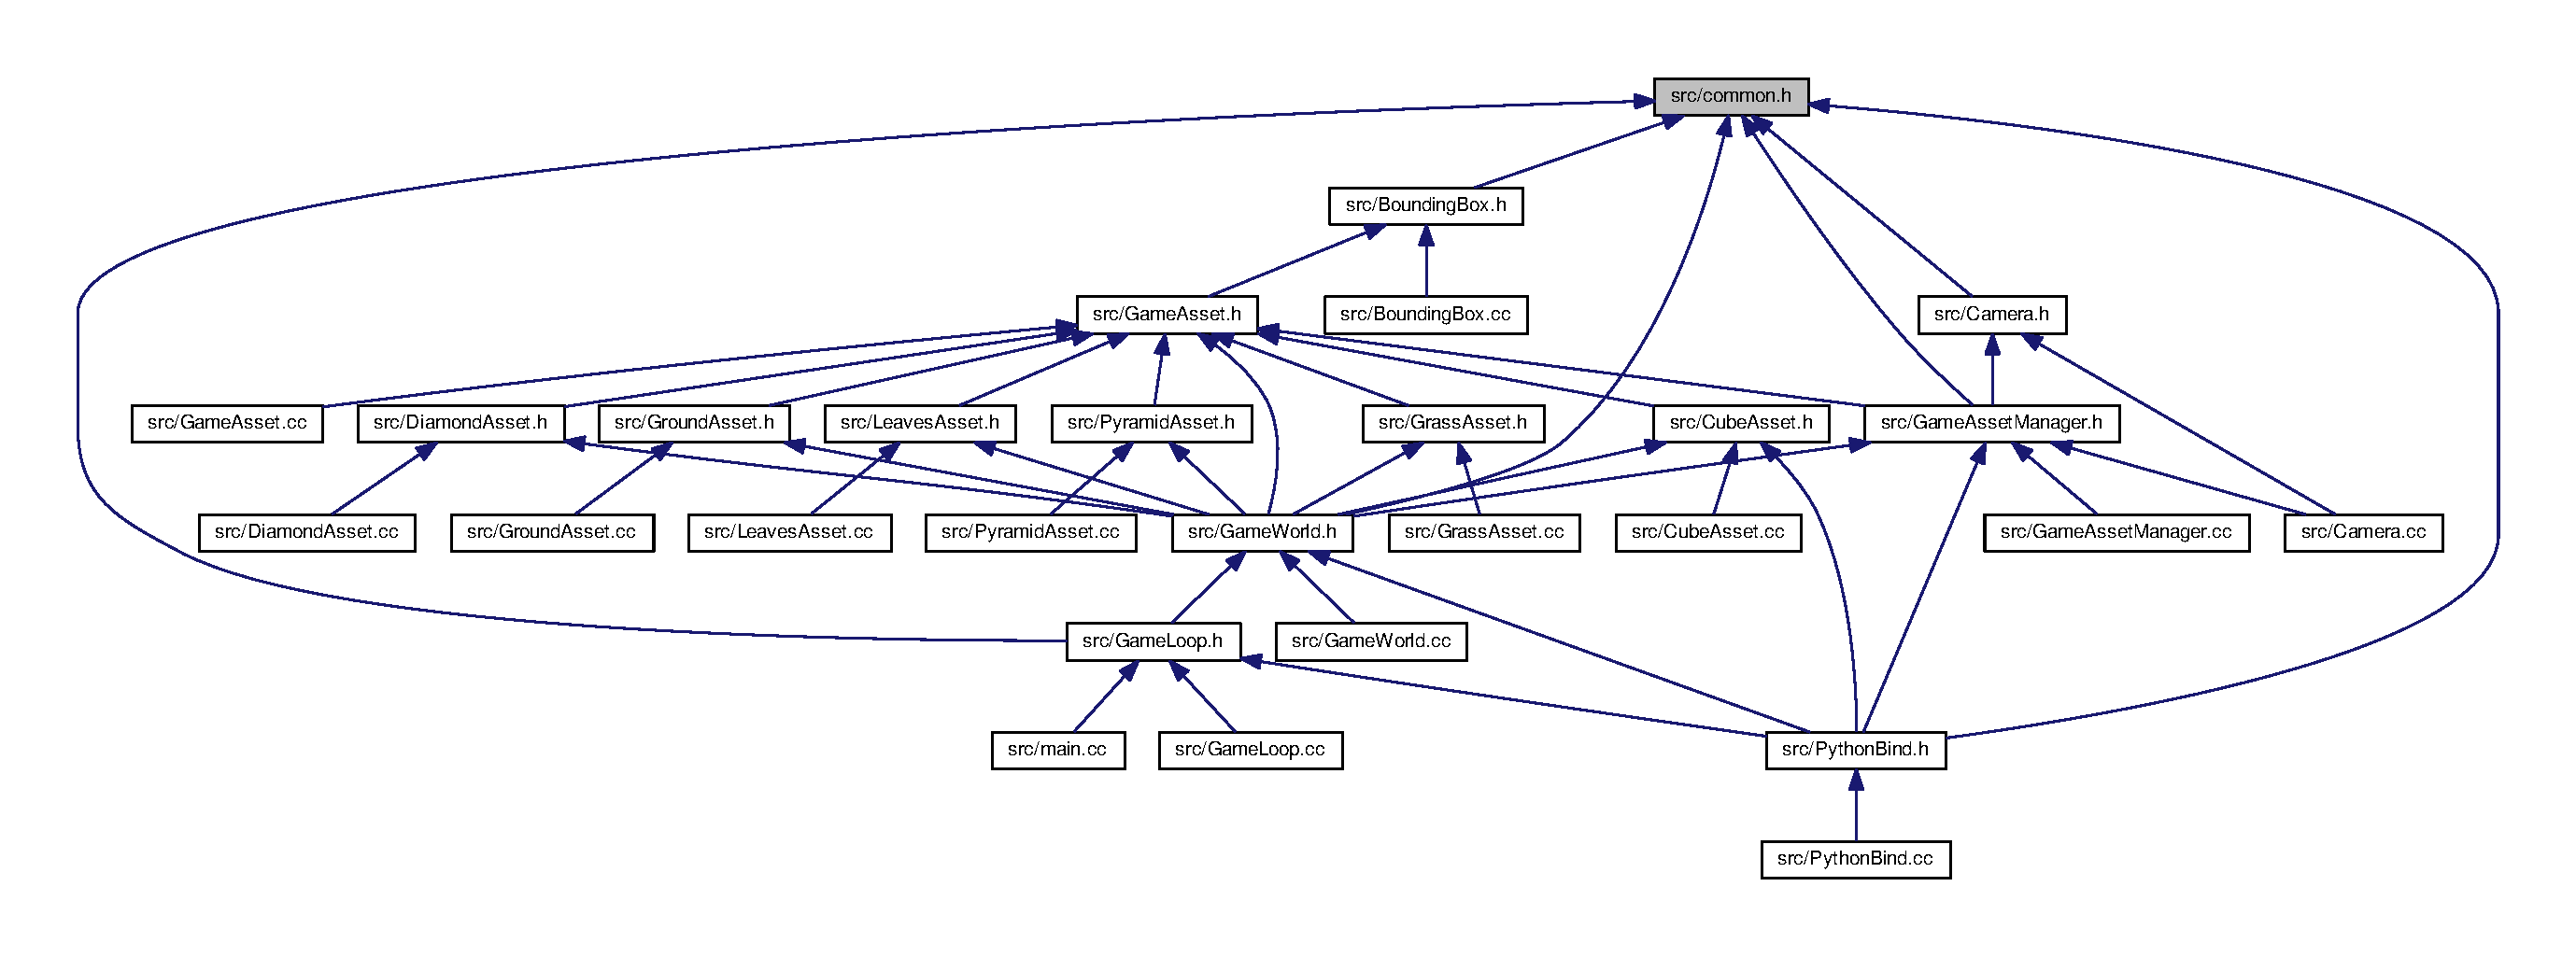
\includegraphics[width=350pt]{common_8h__dep__incl}
\end{center}
\end{figure}
\subsection*{Enumerations}
\begin{DoxyCompactItemize}
\item 
enum \hyperlink{common_8h_a0da83e35f29c11f7f3c637234f2149f9}{Control} \{ \\*
\hyperlink{common_8h_a0da83e35f29c11f7f3c637234f2149f9acdb8b9a398ffbd729218a27d00d8fa45}{N\+O\+T\+\_\+\+P\+R\+E\+S\+S\+E\+D}, 
\hyperlink{common_8h_a0da83e35f29c11f7f3c637234f2149f9aba595d8bca8bc5e67c37c0a9d89becfa}{U\+P}, 
\hyperlink{common_8h_a0da83e35f29c11f7f3c637234f2149f9a9b0b4a95b99523966e0e34ffdadac9da}{D\+O\+W\+N}, 
\hyperlink{common_8h_a0da83e35f29c11f7f3c637234f2149f9adb45120aafd37a973140edee24708065}{L\+E\+F\+T}, 
\\*
\hyperlink{common_8h_a0da83e35f29c11f7f3c637234f2149f9aec8379af7490bb9eaaf579cf17876f38}{R\+I\+G\+H\+T}, 
\hyperlink{common_8h_a0da83e35f29c11f7f3c637234f2149f9a1f28d4392b1c1e7da2af2283632d81e1}{J\+U\+M\+P}, 
\hyperlink{common_8h_a0da83e35f29c11f7f3c637234f2149f9a3cdd4783c5dbeae45bbcd15570a6b273}{C\+R\+O\+U\+C\+H}, 
\hyperlink{common_8h_a0da83e35f29c11f7f3c637234f2149f9ab107229d44d042caa8ab8df4c8acaa1f}{P\+R\+I\+N\+T}
 \}
\end{DoxyCompactItemize}


\subsection{Enumeration Type Documentation}
\hypertarget{common_8h_a0da83e35f29c11f7f3c637234f2149f9}{}\index{common.\+h@{common.\+h}!Control@{Control}}
\index{Control@{Control}!common.\+h@{common.\+h}}
\subsubsection[{Control}]{\setlength{\rightskip}{0pt plus 5cm}enum {\bf Control}}\label{common_8h_a0da83e35f29c11f7f3c637234f2149f9}
Control Control is changed by the last keyboard entry entered \begin{Desc}
\item[Enumerator]\par
\begin{description}
\index{N\+O\+T\+\_\+\+P\+R\+E\+S\+S\+E\+D@{N\+O\+T\+\_\+\+P\+R\+E\+S\+S\+E\+D}!common.\+h@{common.\+h}}\index{common.\+h@{common.\+h}!N\+O\+T\+\_\+\+P\+R\+E\+S\+S\+E\+D@{N\+O\+T\+\_\+\+P\+R\+E\+S\+S\+E\+D}}\item[{\em 
\hypertarget{common_8h_a0da83e35f29c11f7f3c637234f2149f9acdb8b9a398ffbd729218a27d00d8fa45}{}N\+O\+T\+\_\+\+P\+R\+E\+S\+S\+E\+D\label{common_8h_a0da83e35f29c11f7f3c637234f2149f9acdb8b9a398ffbd729218a27d00d8fa45}
}]\index{U\+P@{U\+P}!common.\+h@{common.\+h}}\index{common.\+h@{common.\+h}!U\+P@{U\+P}}\item[{\em 
\hypertarget{common_8h_a0da83e35f29c11f7f3c637234f2149f9aba595d8bca8bc5e67c37c0a9d89becfa}{}U\+P\label{common_8h_a0da83e35f29c11f7f3c637234f2149f9aba595d8bca8bc5e67c37c0a9d89becfa}
}]\index{D\+O\+W\+N@{D\+O\+W\+N}!common.\+h@{common.\+h}}\index{common.\+h@{common.\+h}!D\+O\+W\+N@{D\+O\+W\+N}}\item[{\em 
\hypertarget{common_8h_a0da83e35f29c11f7f3c637234f2149f9a9b0b4a95b99523966e0e34ffdadac9da}{}D\+O\+W\+N\label{common_8h_a0da83e35f29c11f7f3c637234f2149f9a9b0b4a95b99523966e0e34ffdadac9da}
}]\index{L\+E\+F\+T@{L\+E\+F\+T}!common.\+h@{common.\+h}}\index{common.\+h@{common.\+h}!L\+E\+F\+T@{L\+E\+F\+T}}\item[{\em 
\hypertarget{common_8h_a0da83e35f29c11f7f3c637234f2149f9adb45120aafd37a973140edee24708065}{}L\+E\+F\+T\label{common_8h_a0da83e35f29c11f7f3c637234f2149f9adb45120aafd37a973140edee24708065}
}]\index{R\+I\+G\+H\+T@{R\+I\+G\+H\+T}!common.\+h@{common.\+h}}\index{common.\+h@{common.\+h}!R\+I\+G\+H\+T@{R\+I\+G\+H\+T}}\item[{\em 
\hypertarget{common_8h_a0da83e35f29c11f7f3c637234f2149f9aec8379af7490bb9eaaf579cf17876f38}{}R\+I\+G\+H\+T\label{common_8h_a0da83e35f29c11f7f3c637234f2149f9aec8379af7490bb9eaaf579cf17876f38}
}]\index{J\+U\+M\+P@{J\+U\+M\+P}!common.\+h@{common.\+h}}\index{common.\+h@{common.\+h}!J\+U\+M\+P@{J\+U\+M\+P}}\item[{\em 
\hypertarget{common_8h_a0da83e35f29c11f7f3c637234f2149f9a1f28d4392b1c1e7da2af2283632d81e1}{}J\+U\+M\+P\label{common_8h_a0da83e35f29c11f7f3c637234f2149f9a1f28d4392b1c1e7da2af2283632d81e1}
}]\index{C\+R\+O\+U\+C\+H@{C\+R\+O\+U\+C\+H}!common.\+h@{common.\+h}}\index{common.\+h@{common.\+h}!C\+R\+O\+U\+C\+H@{C\+R\+O\+U\+C\+H}}\item[{\em 
\hypertarget{common_8h_a0da83e35f29c11f7f3c637234f2149f9a3cdd4783c5dbeae45bbcd15570a6b273}{}C\+R\+O\+U\+C\+H\label{common_8h_a0da83e35f29c11f7f3c637234f2149f9a3cdd4783c5dbeae45bbcd15570a6b273}
}]\index{P\+R\+I\+N\+T@{P\+R\+I\+N\+T}!common.\+h@{common.\+h}}\index{common.\+h@{common.\+h}!P\+R\+I\+N\+T@{P\+R\+I\+N\+T}}\item[{\em 
\hypertarget{common_8h_a0da83e35f29c11f7f3c637234f2149f9ab107229d44d042caa8ab8df4c8acaa1f}{}P\+R\+I\+N\+T\label{common_8h_a0da83e35f29c11f7f3c637234f2149f9ab107229d44d042caa8ab8df4c8acaa1f}
}]\end{description}
\end{Desc}

\begin{DoxyCode}
8 \{\hyperlink{common_8h_a0da83e35f29c11f7f3c637234f2149f9acdb8b9a398ffbd729218a27d00d8fa45}{NOT\_PRESSED}, \hyperlink{common_8h_a0da83e35f29c11f7f3c637234f2149f9aba595d8bca8bc5e67c37c0a9d89becfa}{UP}, \hyperlink{common_8h_a0da83e35f29c11f7f3c637234f2149f9a9b0b4a95b99523966e0e34ffdadac9da}{DOWN}, \hyperlink{common_8h_a0da83e35f29c11f7f3c637234f2149f9adb45120aafd37a973140edee24708065}{LEFT}, \hyperlink{common_8h_a0da83e35f29c11f7f3c637234f2149f9aec8379af7490bb9eaaf579cf17876f38}{RIGHT}, \hyperlink{common_8h_a0da83e35f29c11f7f3c637234f2149f9a1f28d4392b1c1e7da2af2283632d81e1}{JUMP}, \hyperlink{common_8h_a0da83e35f29c11f7f3c637234f2149f9a3cdd4783c5dbeae45bbcd15570a6b273}{CROUCH}, 
      \hyperlink{common_8h_a0da83e35f29c11f7f3c637234f2149f9ab107229d44d042caa8ab8df4c8acaa1f}{PRINT}\};
\end{DoxyCode}

\hypertarget{CubeAsset_8cc}{}\section{src/\+Cube\+Asset.cc File Reference}
\label{CubeAsset_8cc}\index{src/\+Cube\+Asset.\+cc@{src/\+Cube\+Asset.\+cc}}
{\ttfamily \#include \char`\"{}Cube\+Asset.\+h\char`\"{}}\\*
Include dependency graph for Cube\+Asset.\+cc\+:
\nopagebreak
\begin{figure}[H]
\begin{center}
\leavevmode
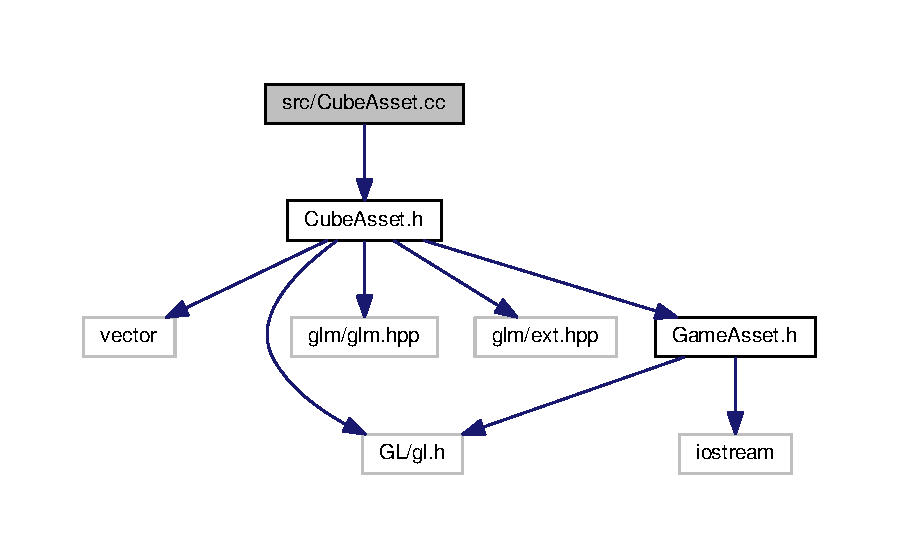
\includegraphics[width=350pt]{CubeAsset_8cc__incl}
\end{center}
\end{figure}
\subsection*{Macros}
\begin{DoxyCompactItemize}
\item 
\#define \hyperlink{CubeAsset_8cc_a75f201b0e53e68726854997957322b8d}{check\+G\+L\+Error}()
\end{DoxyCompactItemize}
\subsection*{Functions}
\begin{DoxyCompactItemize}
\item 
void \hyperlink{CubeAsset_8cc_abe4ebf09b25b6e092e65ce01e73987d7}{check\+Error} (std\+::string file, int line)
\end{DoxyCompactItemize}


\subsection{Macro Definition Documentation}
\hypertarget{CubeAsset_8cc_a75f201b0e53e68726854997957322b8d}{}\index{Cube\+Asset.\+cc@{Cube\+Asset.\+cc}!check\+G\+L\+Error@{check\+G\+L\+Error}}
\index{check\+G\+L\+Error@{check\+G\+L\+Error}!Cube\+Asset.\+cc@{Cube\+Asset.\+cc}}
\subsubsection[{check\+G\+L\+Error}]{\setlength{\rightskip}{0pt plus 5cm}\#define check\+G\+L\+Error(
\begin{DoxyParamCaption}
{}
\end{DoxyParamCaption}
)}\label{CubeAsset_8cc_a75f201b0e53e68726854997957322b8d}


\subsection{Function Documentation}
\hypertarget{CubeAsset_8cc_abe4ebf09b25b6e092e65ce01e73987d7}{}\index{Cube\+Asset.\+cc@{Cube\+Asset.\+cc}!check\+Error@{check\+Error}}
\index{check\+Error@{check\+Error}!Cube\+Asset.\+cc@{Cube\+Asset.\+cc}}
\subsubsection[{check\+Error(std\+::string file, int line)}]{\setlength{\rightskip}{0pt plus 5cm}void check\+Error (
\begin{DoxyParamCaption}
\item[{std\+::string}]{file, }
\item[{int}]{line}
\end{DoxyParamCaption}
)}\label{CubeAsset_8cc_abe4ebf09b25b6e092e65ce01e73987d7}

\begin{DoxyCode}
91                                           \{
92   GLenum gl\_error = glGetError();
93   \textcolor{keywordflow}{if}(GL\_NO\_ERROR != gl\_error) \{
94     std::cerr << \textcolor{stringliteral}{"GL error in "} << file << \textcolor{stringliteral}{" at line "} << line << \textcolor{stringliteral}{" error: "} << gl\_error << std::endl;
95     exit(-1);
96   \}
97 \}
\end{DoxyCode}

\hypertarget{CubeAsset_8h}{}\section{src/\+Cube\+Asset.h File Reference}
\label{CubeAsset_8h}\index{src/\+Cube\+Asset.\+h@{src/\+Cube\+Asset.\+h}}
{\ttfamily \#include $<$vector$>$}\\*
{\ttfamily \#include $<$G\+L/gl.\+h$>$}\\*
{\ttfamily \#include $<$glm/glm.\+hpp$>$}\\*
{\ttfamily \#include $<$glm/ext.\+hpp$>$}\\*
{\ttfamily \#include \char`\"{}Game\+Asset.\+h\char`\"{}}\\*
Include dependency graph for Cube\+Asset.\+h\+:\nopagebreak
\begin{figure}[H]
\begin{center}
\leavevmode
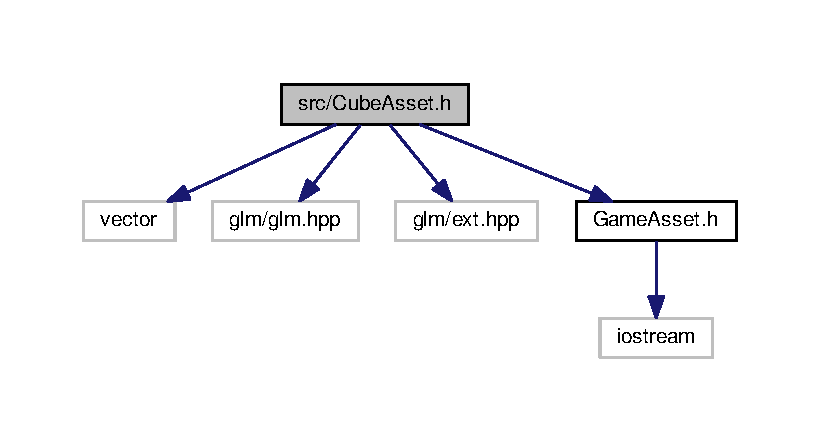
\includegraphics[width=350pt]{CubeAsset_8h__incl}
\end{center}
\end{figure}
This graph shows which files directly or indirectly include this file\+:\nopagebreak
\begin{figure}[H]
\begin{center}
\leavevmode
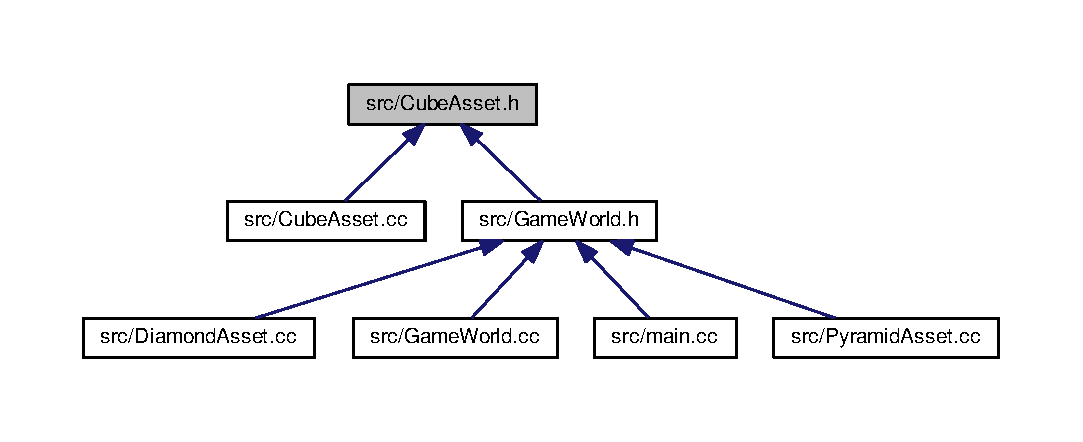
\includegraphics[width=350pt]{CubeAsset_8h__dep__incl}
\end{center}
\end{figure}
\subsection*{Classes}
\begin{DoxyCompactItemize}
\item 
class \hyperlink{classCubeAsset}{Cube\+Asset}
\end{DoxyCompactItemize}

\hypertarget{DiamondAsset_8cc}{}\section{src/\+Diamond\+Asset.cc File Reference}
\label{DiamondAsset_8cc}\index{src/\+Diamond\+Asset.\+cc@{src/\+Diamond\+Asset.\+cc}}
{\ttfamily \#include \char`\"{}Diamond\+Asset.\+h\char`\"{}}\\*
Include dependency graph for Diamond\+Asset.\+cc\+:\nopagebreak
\begin{figure}[H]
\begin{center}
\leavevmode
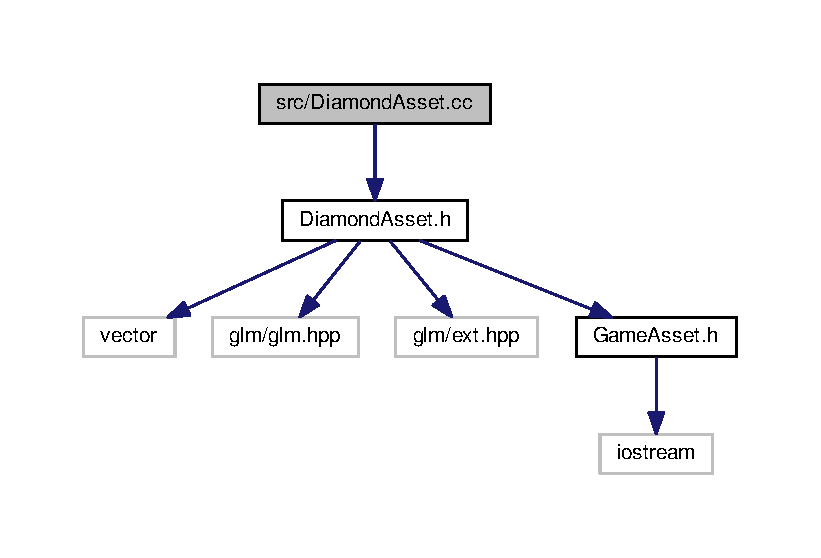
\includegraphics[width=350pt]{DiamondAsset_8cc__incl}
\end{center}
\end{figure}
\subsection*{Macros}
\begin{DoxyCompactItemize}
\item 
\#define \hyperlink{DiamondAsset_8cc_a75f201b0e53e68726854997957322b8d}{check\+G\+L\+Error}()
\end{DoxyCompactItemize}


\subsection{Macro Definition Documentation}
\hypertarget{DiamondAsset_8cc_a75f201b0e53e68726854997957322b8d}{}\index{Diamond\+Asset.\+cc@{Diamond\+Asset.\+cc}!check\+G\+L\+Error@{check\+G\+L\+Error}}
\index{check\+G\+L\+Error@{check\+G\+L\+Error}!Diamond\+Asset.\+cc@{Diamond\+Asset.\+cc}}
\subsubsection[{check\+G\+L\+Error}]{\setlength{\rightskip}{0pt plus 5cm}\#define check\+G\+L\+Error(
\begin{DoxyParamCaption}
{}
\end{DoxyParamCaption}
)}\label{DiamondAsset_8cc_a75f201b0e53e68726854997957322b8d}

\hypertarget{DiamondAsset_8h}{}\section{src/\+Diamond\+Asset.h File Reference}
\label{DiamondAsset_8h}\index{src/\+Diamond\+Asset.\+h@{src/\+Diamond\+Asset.\+h}}
{\ttfamily \#include $<$vector$>$}\\*
{\ttfamily \#include $<$glm/glm.\+hpp$>$}\\*
{\ttfamily \#include $<$glm/ext.\+hpp$>$}\\*
{\ttfamily \#include \char`\"{}Game\+Asset.\+h\char`\"{}}\\*
Include dependency graph for Diamond\+Asset.\+h\+:
\nopagebreak
\begin{figure}[H]
\begin{center}
\leavevmode
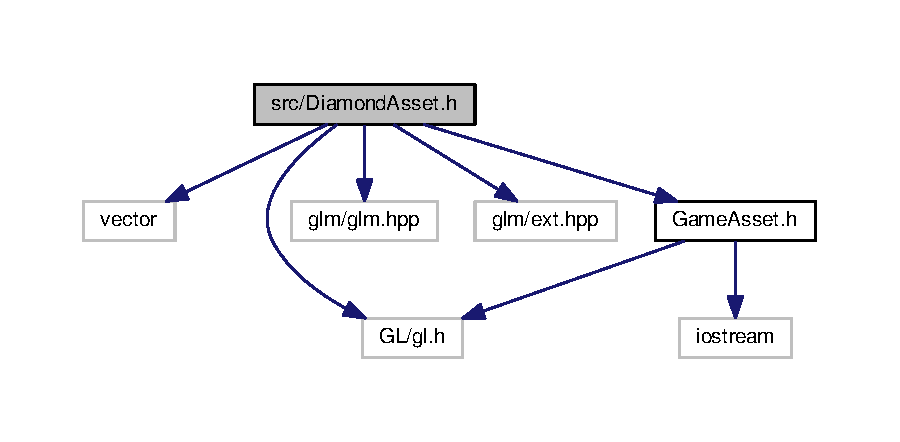
\includegraphics[width=350pt]{DiamondAsset_8h__incl}
\end{center}
\end{figure}
This graph shows which files directly or indirectly include this file\+:\nopagebreak
\begin{figure}[H]
\begin{center}
\leavevmode
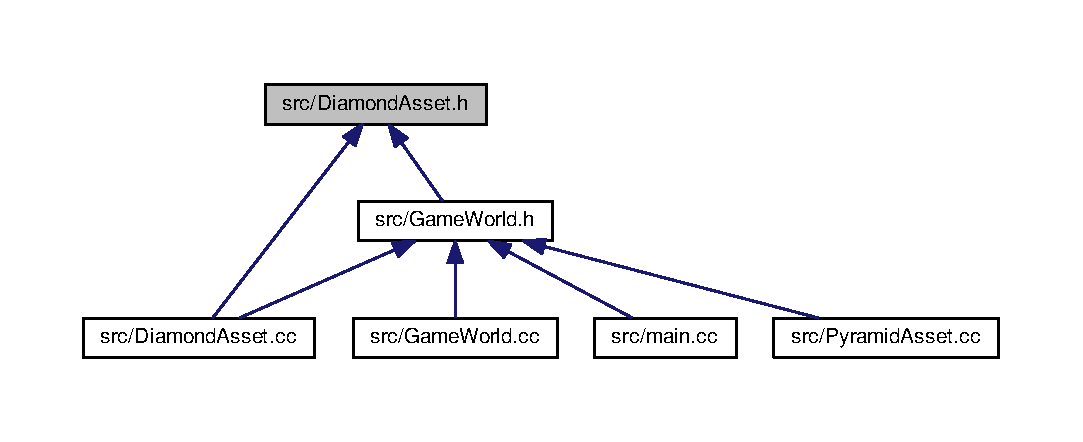
\includegraphics[width=340pt]{DiamondAsset_8h__dep__incl}
\end{center}
\end{figure}
\subsection*{Classes}
\begin{DoxyCompactItemize}
\item 
class \hyperlink{classDiamondAsset}{Diamond\+Asset}
\end{DoxyCompactItemize}

\hypertarget{GameAsset_8h}{}\section{src/\+Game\+Asset.h File Reference}
\label{GameAsset_8h}\index{src/\+Game\+Asset.\+h@{src/\+Game\+Asset.\+h}}
{\ttfamily \#include $<$iostream$>$}\\*
Include dependency graph for Game\+Asset.\+h\+:
\nopagebreak
\begin{figure}[H]
\begin{center}
\leavevmode
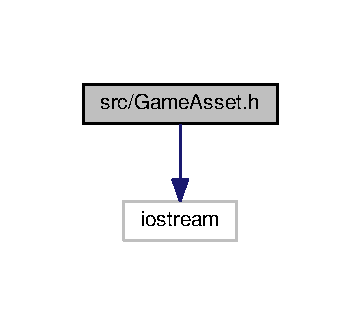
\includegraphics[width=173pt]{GameAsset_8h__incl}
\end{center}
\end{figure}
This graph shows which files directly or indirectly include this file\+:\nopagebreak
\begin{figure}[H]
\begin{center}
\leavevmode
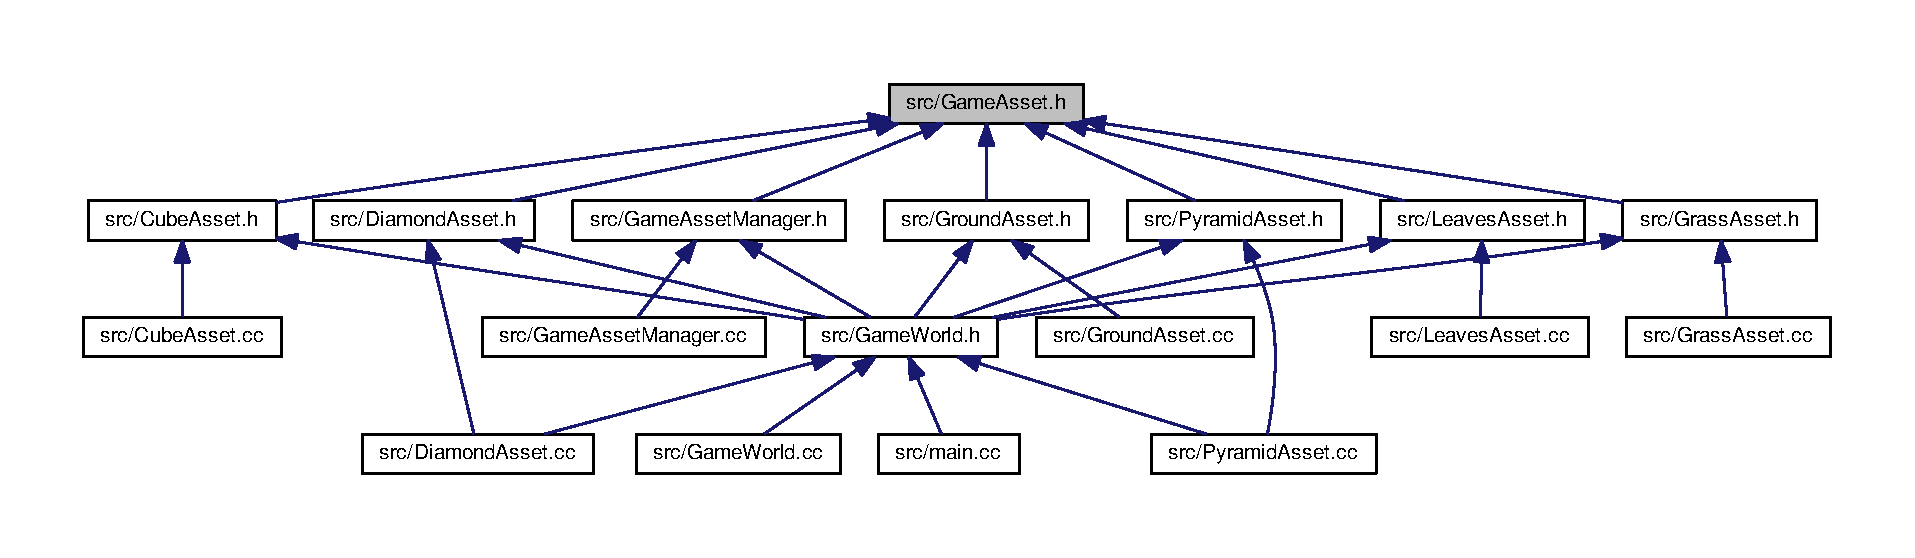
\includegraphics[width=350pt]{GameAsset_8h__dep__incl}
\end{center}
\end{figure}
\subsection*{Classes}
\begin{DoxyCompactItemize}
\item 
class \hyperlink{classGameAsset}{Game\+Asset}
\end{DoxyCompactItemize}

\hypertarget{GameAssetManager_8cc}{}\section{src/\+Game\+Asset\+Manager.cc File Reference}
\label{GameAssetManager_8cc}\index{src/\+Game\+Asset\+Manager.\+cc@{src/\+Game\+Asset\+Manager.\+cc}}
{\ttfamily \#include \char`\"{}Game\+Asset\+Manager.\+h\char`\"{}}\\*
Include dependency graph for Game\+Asset\+Manager.\+cc\+:\nopagebreak
\begin{figure}[H]
\begin{center}
\leavevmode
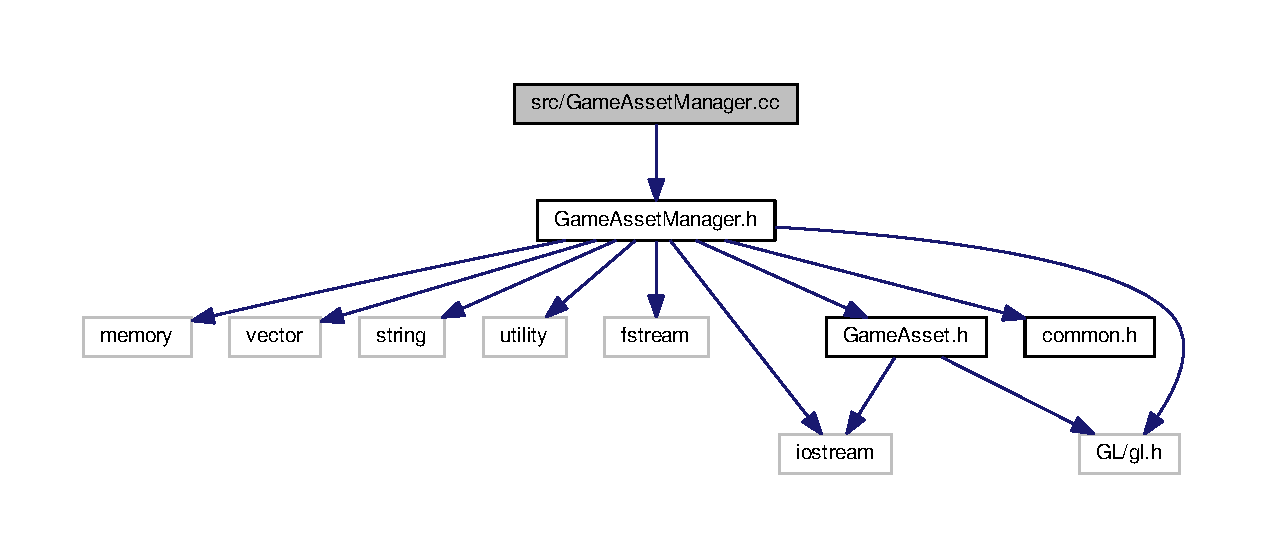
\includegraphics[width=350pt]{GameAssetManager_8cc__incl}
\end{center}
\end{figure}

\hypertarget{GameAssetManager_8h}{}\section{src/\+Game\+Asset\+Manager.h File Reference}
\label{GameAssetManager_8h}\index{src/\+Game\+Asset\+Manager.\+h@{src/\+Game\+Asset\+Manager.\+h}}
{\ttfamily \#include $<$memory$>$}\\*
{\ttfamily \#include $<$vector$>$}\\*
{\ttfamily \#include $<$string$>$}\\*
{\ttfamily \#include $<$utility$>$}\\*
{\ttfamily \#include $<$fstream$>$}\\*
{\ttfamily \#include $<$iostream$>$}\\*
{\ttfamily \#include \char`\"{}common.\+h\char`\"{}}\\*
{\ttfamily \#include \char`\"{}Game\+Asset.\+h\char`\"{}}\\*
Include dependency graph for Game\+Asset\+Manager.\+h\+:\nopagebreak
\begin{figure}[H]
\begin{center}
\leavevmode
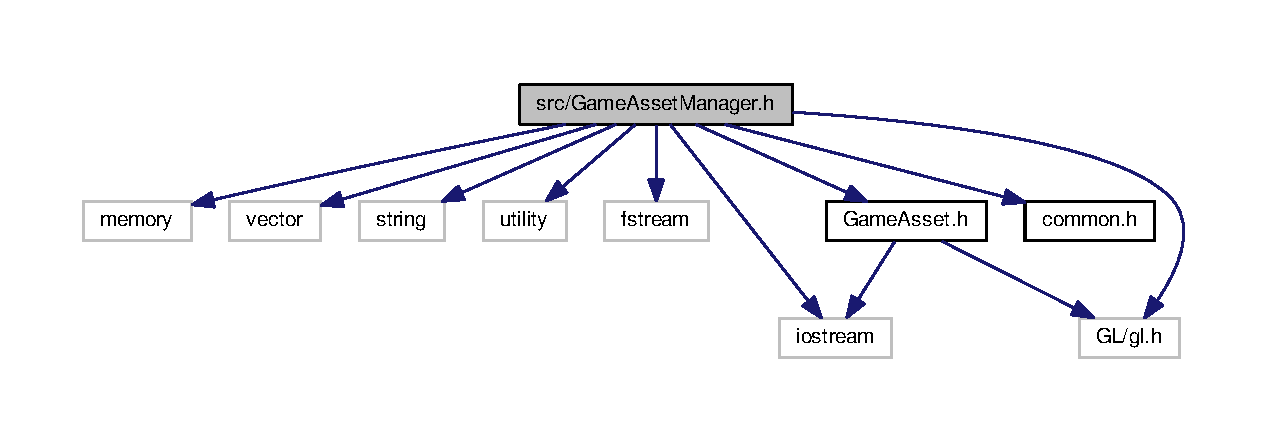
\includegraphics[width=350pt]{GameAssetManager_8h__incl}
\end{center}
\end{figure}
This graph shows which files directly or indirectly include this file\+:\nopagebreak
\begin{figure}[H]
\begin{center}
\leavevmode
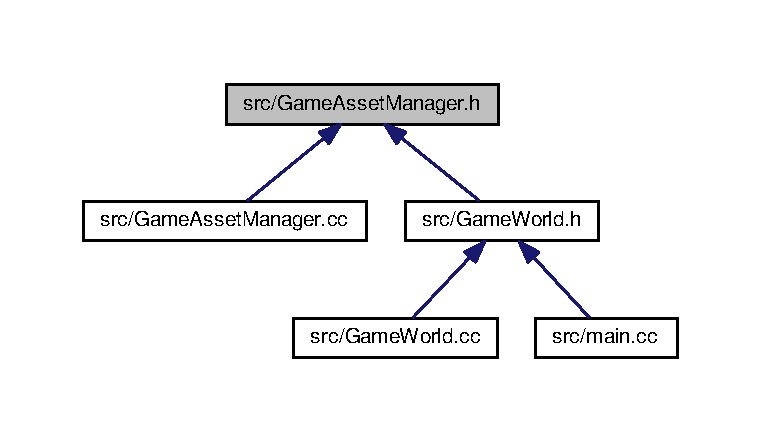
\includegraphics[width=350pt]{GameAssetManager_8h__dep__incl}
\end{center}
\end{figure}
\subsection*{Classes}
\begin{DoxyCompactItemize}
\item 
class \hyperlink{classGameAssetManager}{Game\+Asset\+Manager}
\begin{DoxyCompactList}\small\item\em \hyperlink{classGameAssetManager}{Game\+Asset\+Manager} is a container for Game\+Assets. \end{DoxyCompactList}\end{DoxyCompactItemize}

\hypertarget{GameWorld_8cc}{}\section{src/\+Game\+World.cc File Reference}
\label{GameWorld_8cc}\index{src/\+Game\+World.\+cc@{src/\+Game\+World.\+cc}}
{\ttfamily \#include \char`\"{}Game\+World.\+h\char`\"{}}\\*
{\ttfamily \#include \char`\"{}common.\+h\char`\"{}}\\*

\hypertarget{GameWorld_8h}{}\section{src/\+Game\+World.h File Reference}
\label{GameWorld_8h}\index{src/\+Game\+World.\+h@{src/\+Game\+World.\+h}}
{\ttfamily \#include $<$memory$>$}\\*
{\ttfamily \#include $<$G\+L/gl.\+h$>$}\\*
{\ttfamily \#include \char`\"{}common.\+h\char`\"{}}\\*
{\ttfamily \#include \char`\"{}Game\+Asset\+Manager.\+h\char`\"{}}\\*
{\ttfamily \#include \char`\"{}Cube\+Asset.\+h\char`\"{}}\\*
{\ttfamily \#include \char`\"{}Diamond\+Asset.\+h\char`\"{}}\\*
{\ttfamily \#include \char`\"{}Ground\+Asset.\+h\char`\"{}}\\*
{\ttfamily \#include \char`\"{}Leaves\+Asset.\+h\char`\"{}}\\*
{\ttfamily \#include \char`\"{}Pyramid\+Asset.\+h\char`\"{}}\\*
{\ttfamily \#include \char`\"{}Grass\+Asset.\+h\char`\"{}}\\*
Include dependency graph for Game\+World.\+h\+:\nopagebreak
\begin{figure}[H]
\begin{center}
\leavevmode
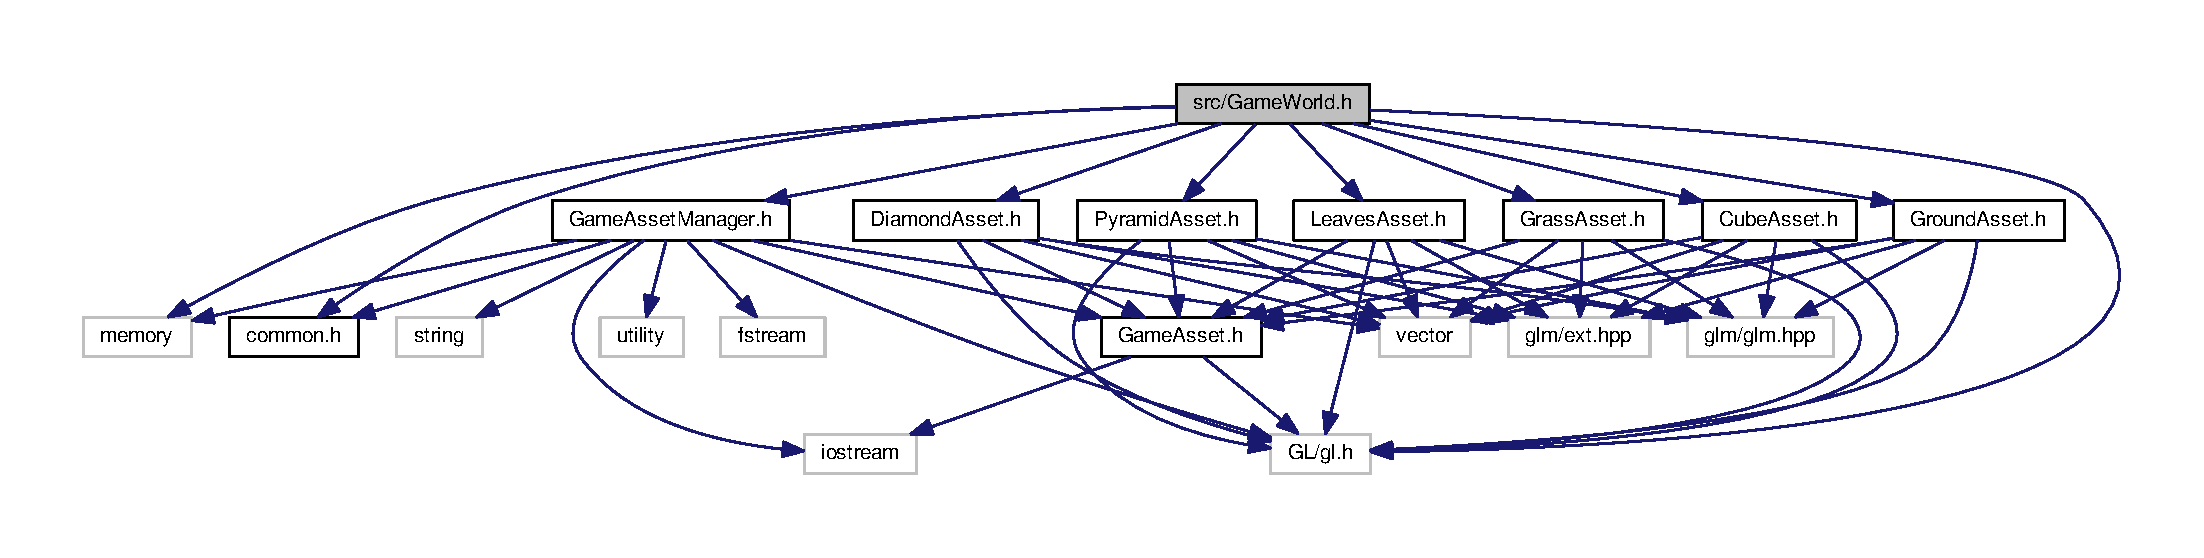
\includegraphics[width=350pt]{GameWorld_8h__incl}
\end{center}
\end{figure}
This graph shows which files directly or indirectly include this file\+:
\nopagebreak
\begin{figure}[H]
\begin{center}
\leavevmode
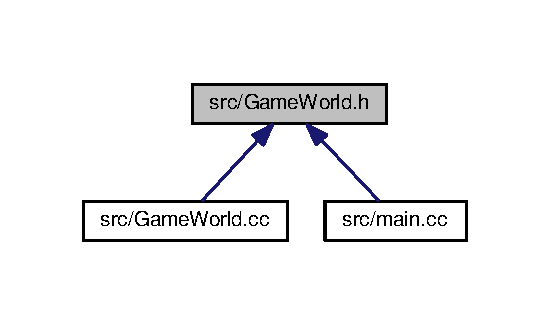
\includegraphics[width=264pt]{GameWorld_8h__dep__incl}
\end{center}
\end{figure}
\subsection*{Classes}
\begin{DoxyCompactItemize}
\item 
class \hyperlink{classGameWorld}{Game\+World}
\end{DoxyCompactItemize}

\hypertarget{GrassAsset_8cc}{}\section{src/\+Grass\+Asset.cc File Reference}
\label{GrassAsset_8cc}\index{src/\+Grass\+Asset.\+cc@{src/\+Grass\+Asset.\+cc}}
{\ttfamily \#include \char`\"{}Grass\+Asset.\+h\char`\"{}}\\*
Include dependency graph for Grass\+Asset.\+cc\+:\nopagebreak
\begin{figure}[H]
\begin{center}
\leavevmode
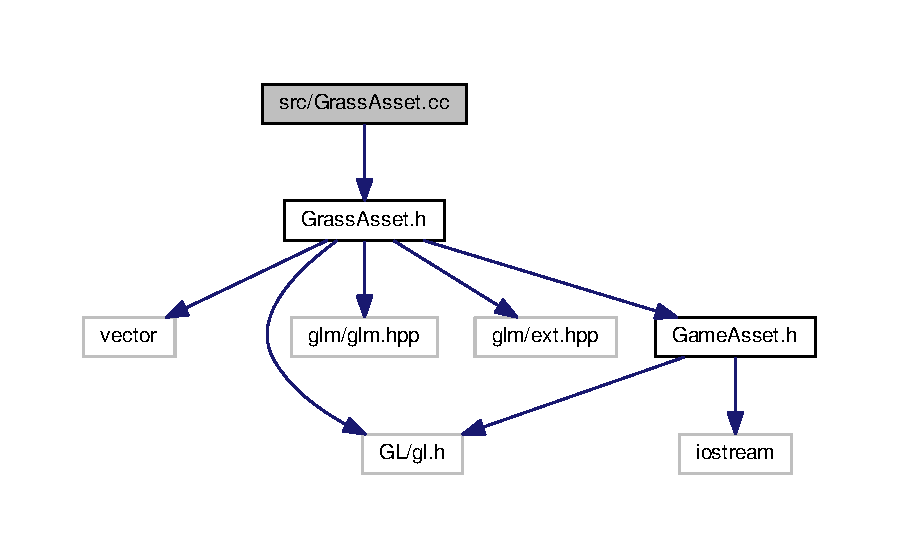
\includegraphics[width=350pt]{GrassAsset_8cc__incl}
\end{center}
\end{figure}
\subsection*{Macros}
\begin{DoxyCompactItemize}
\item 
\#define \hyperlink{GrassAsset_8cc_a75f201b0e53e68726854997957322b8d}{check\+G\+L\+Error}()
\begin{DoxyCompactList}\small\item\em define symbol to be nothing \end{DoxyCompactList}\end{DoxyCompactItemize}


\subsection{Macro Definition Documentation}
\hypertarget{GrassAsset_8cc_a75f201b0e53e68726854997957322b8d}{}\index{Grass\+Asset.\+cc@{Grass\+Asset.\+cc}!check\+G\+L\+Error@{check\+G\+L\+Error}}
\index{check\+G\+L\+Error@{check\+G\+L\+Error}!Grass\+Asset.\+cc@{Grass\+Asset.\+cc}}
\subsubsection[{check\+G\+L\+Error}]{\setlength{\rightskip}{0pt plus 5cm}\#define check\+G\+L\+Error(
\begin{DoxyParamCaption}
{}
\end{DoxyParamCaption}
)}\label{GrassAsset_8cc_a75f201b0e53e68726854997957322b8d}


define symbol to be nothing 


\hypertarget{GrassAsset_8h}{}\section{src/\+Grass\+Asset.h File Reference}
\label{GrassAsset_8h}\index{src/\+Grass\+Asset.\+h@{src/\+Grass\+Asset.\+h}}
{\ttfamily \#include $<$vector$>$}\\*
{\ttfamily \#include $<$glm/glm.\+hpp$>$}\\*
{\ttfamily \#include $<$glm/ext.\+hpp$>$}\\*
{\ttfamily \#include \char`\"{}Game\+Asset.\+h\char`\"{}}\\*
Include dependency graph for Grass\+Asset.\+h\+:\nopagebreak
\begin{figure}[H]
\begin{center}
\leavevmode
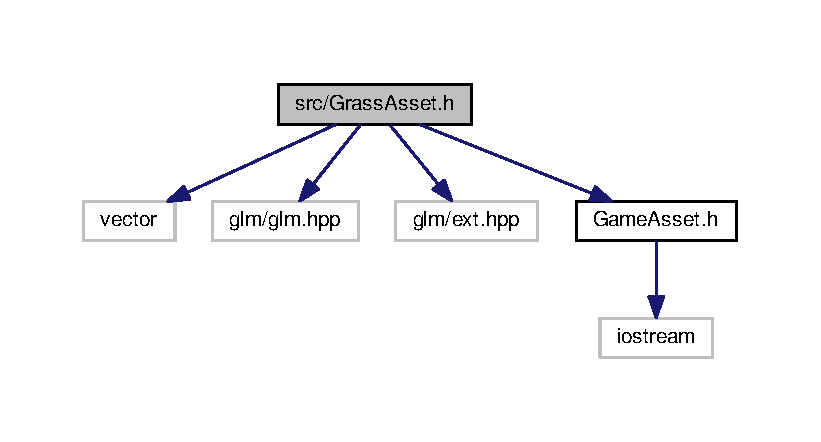
\includegraphics[width=350pt]{GrassAsset_8h__incl}
\end{center}
\end{figure}
This graph shows which files directly or indirectly include this file\+:\nopagebreak
\begin{figure}[H]
\begin{center}
\leavevmode
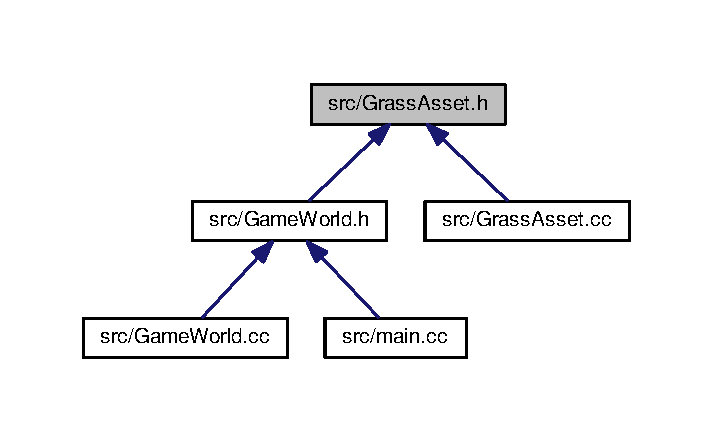
\includegraphics[width=342pt]{GrassAsset_8h__dep__incl}
\end{center}
\end{figure}
\subsection*{Classes}
\begin{DoxyCompactItemize}
\item 
class \hyperlink{classGrassAsset}{Grass\+Asset}
\end{DoxyCompactItemize}

\hypertarget{GroundAsset_8cc}{}\section{src/\+Ground\+Asset.cc File Reference}
\label{GroundAsset_8cc}\index{src/\+Ground\+Asset.\+cc@{src/\+Ground\+Asset.\+cc}}
{\ttfamily \#include \char`\"{}Ground\+Asset.\+h\char`\"{}}\\*
Include dependency graph for Ground\+Asset.\+cc\+:
\nopagebreak
\begin{figure}[H]
\begin{center}
\leavevmode
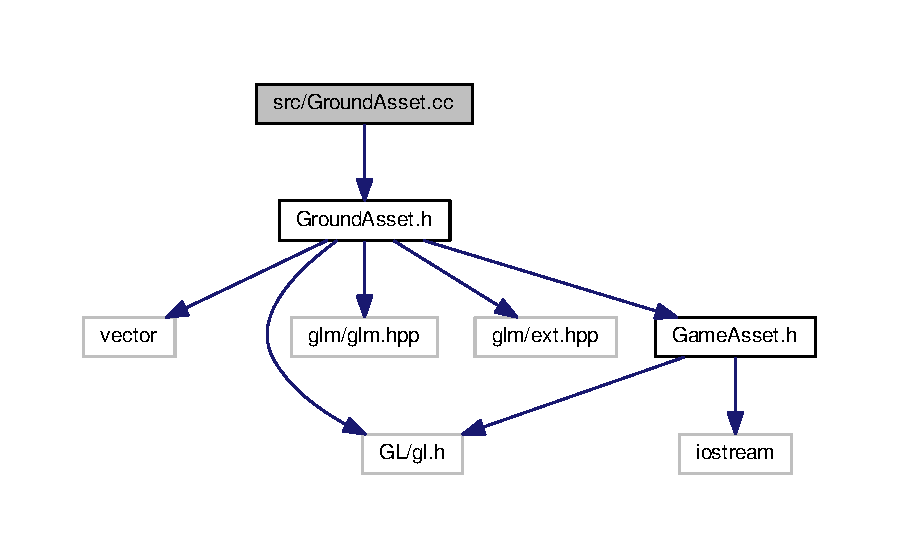
\includegraphics[width=350pt]{GroundAsset_8cc__incl}
\end{center}
\end{figure}
\subsection*{Macros}
\begin{DoxyCompactItemize}
\item 
\#define \hyperlink{GroundAsset_8cc_a75f201b0e53e68726854997957322b8d}{check\+G\+L\+Error}()
\end{DoxyCompactItemize}


\subsection{Macro Definition Documentation}
\hypertarget{GroundAsset_8cc_a75f201b0e53e68726854997957322b8d}{}\index{Ground\+Asset.\+cc@{Ground\+Asset.\+cc}!check\+G\+L\+Error@{check\+G\+L\+Error}}
\index{check\+G\+L\+Error@{check\+G\+L\+Error}!Ground\+Asset.\+cc@{Ground\+Asset.\+cc}}
\subsubsection[{check\+G\+L\+Error}]{\setlength{\rightskip}{0pt plus 5cm}\#define check\+G\+L\+Error(
\begin{DoxyParamCaption}
{}
\end{DoxyParamCaption}
)}\label{GroundAsset_8cc_a75f201b0e53e68726854997957322b8d}

\hypertarget{GroundAsset_8h}{}\section{src/\+Ground\+Asset.h File Reference}
\label{GroundAsset_8h}\index{src/\+Ground\+Asset.\+h@{src/\+Ground\+Asset.\+h}}
{\ttfamily \#include $<$vector$>$}\\*
{\ttfamily \#include $<$G\+L/gl.\+h$>$}\\*
{\ttfamily \#include $<$glm/glm.\+hpp$>$}\\*
{\ttfamily \#include $<$glm/ext.\+hpp$>$}\\*
{\ttfamily \#include \char`\"{}Game\+Asset.\+h\char`\"{}}\\*
Include dependency graph for Ground\+Asset.\+h\+:\nopagebreak
\begin{figure}[H]
\begin{center}
\leavevmode
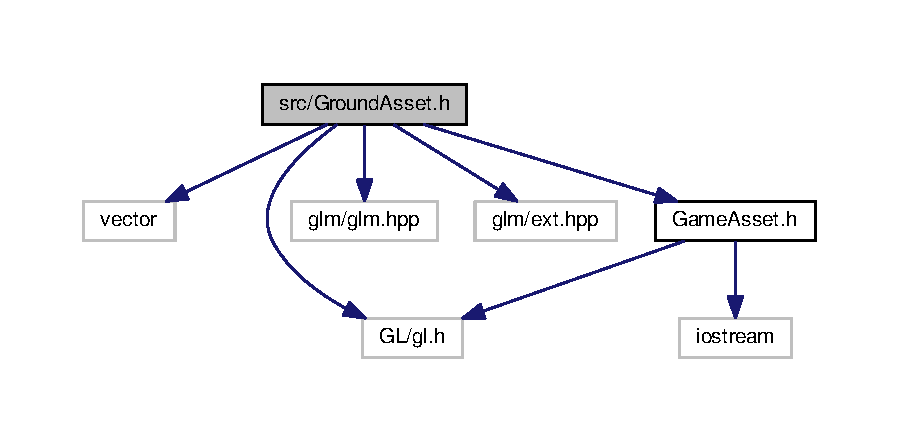
\includegraphics[width=350pt]{GroundAsset_8h__incl}
\end{center}
\end{figure}
This graph shows which files directly or indirectly include this file\+:
\nopagebreak
\begin{figure}[H]
\begin{center}
\leavevmode
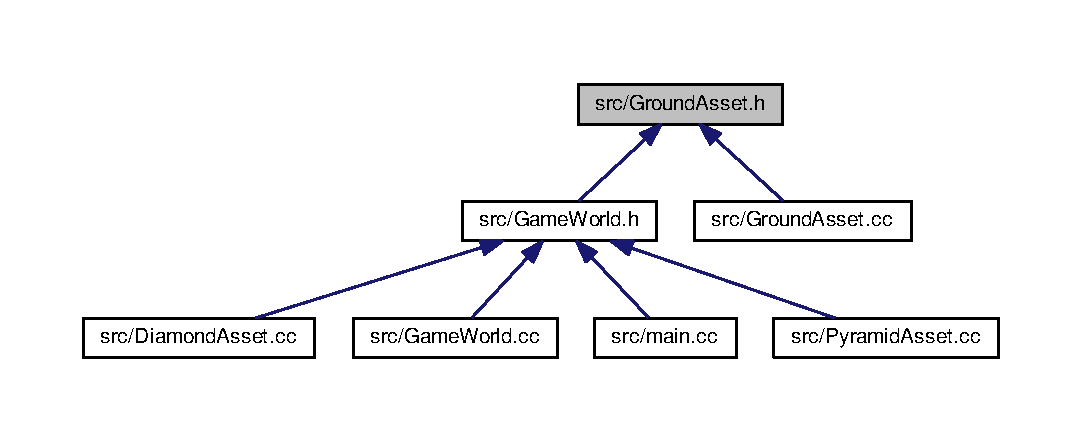
\includegraphics[width=348pt]{GroundAsset_8h__dep__incl}
\end{center}
\end{figure}
\subsection*{Classes}
\begin{DoxyCompactItemize}
\item 
class \hyperlink{classGroundAsset}{Ground\+Asset}
\end{DoxyCompactItemize}

\hypertarget{LeavesAsset_8cc}{}\section{src/\+Leaves\+Asset.cc File Reference}
\label{LeavesAsset_8cc}\index{src/\+Leaves\+Asset.\+cc@{src/\+Leaves\+Asset.\+cc}}
{\ttfamily \#include \char`\"{}Leaves\+Asset.\+h\char`\"{}}\\*
Include dependency graph for Leaves\+Asset.\+cc\+:\nopagebreak
\begin{figure}[H]
\begin{center}
\leavevmode
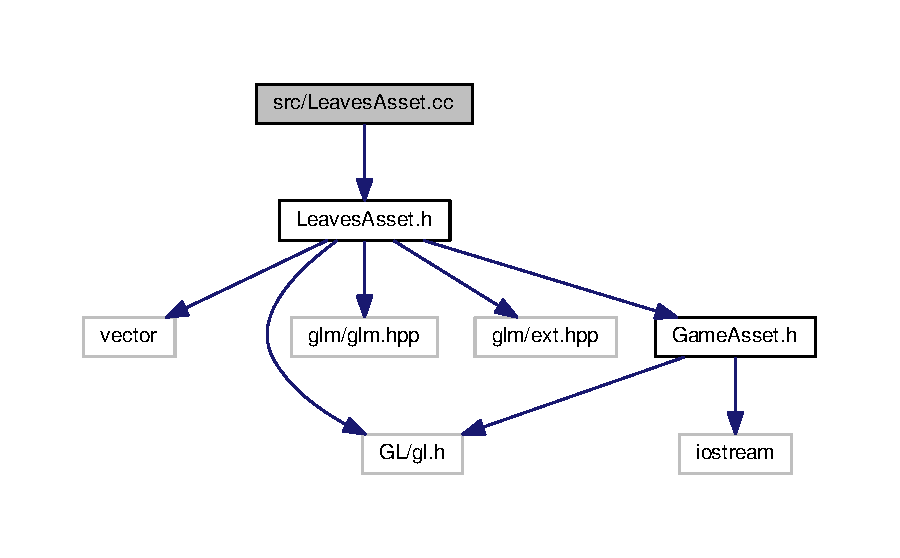
\includegraphics[width=350pt]{LeavesAsset_8cc__incl}
\end{center}
\end{figure}
\subsection*{Macros}
\begin{DoxyCompactItemize}
\item 
\#define \hyperlink{LeavesAsset_8cc_a75f201b0e53e68726854997957322b8d}{check\+G\+L\+Error}()
\begin{DoxyCompactList}\small\item\em define symbol to be nothing \end{DoxyCompactList}\end{DoxyCompactItemize}


\subsection{Macro Definition Documentation}
\hypertarget{LeavesAsset_8cc_a75f201b0e53e68726854997957322b8d}{}\index{Leaves\+Asset.\+cc@{Leaves\+Asset.\+cc}!check\+G\+L\+Error@{check\+G\+L\+Error}}
\index{check\+G\+L\+Error@{check\+G\+L\+Error}!Leaves\+Asset.\+cc@{Leaves\+Asset.\+cc}}
\subsubsection[{check\+G\+L\+Error}]{\setlength{\rightskip}{0pt plus 5cm}\#define check\+G\+L\+Error(
\begin{DoxyParamCaption}
{}
\end{DoxyParamCaption}
)}\label{LeavesAsset_8cc_a75f201b0e53e68726854997957322b8d}


define symbol to be nothing 


\hypertarget{LeavesAsset_8h}{}\section{src/\+Leaves\+Asset.h File Reference}
\label{LeavesAsset_8h}\index{src/\+Leaves\+Asset.\+h@{src/\+Leaves\+Asset.\+h}}
{\ttfamily \#include $<$vector$>$}\\*
{\ttfamily \#include $<$glm/glm.\+hpp$>$}\\*
{\ttfamily \#include $<$glm/ext.\+hpp$>$}\\*
{\ttfamily \#include \char`\"{}Game\+Asset.\+h\char`\"{}}\\*
Include dependency graph for Leaves\+Asset.\+h\+:\nopagebreak
\begin{figure}[H]
\begin{center}
\leavevmode
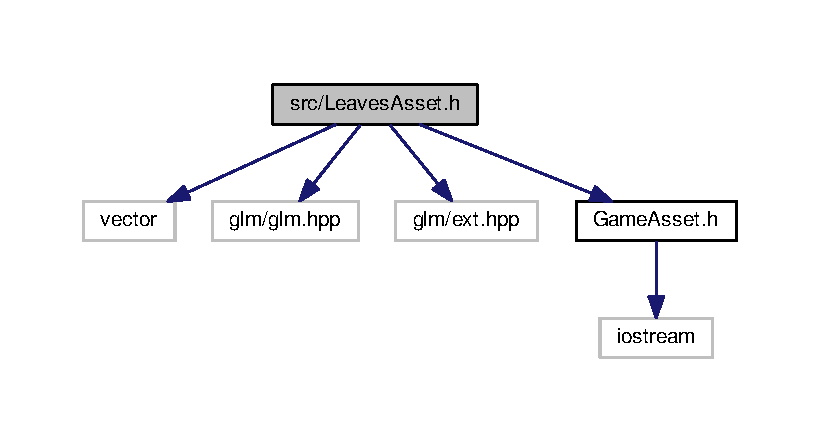
\includegraphics[width=350pt]{LeavesAsset_8h__incl}
\end{center}
\end{figure}
This graph shows which files directly or indirectly include this file\+:\nopagebreak
\begin{figure}[H]
\begin{center}
\leavevmode
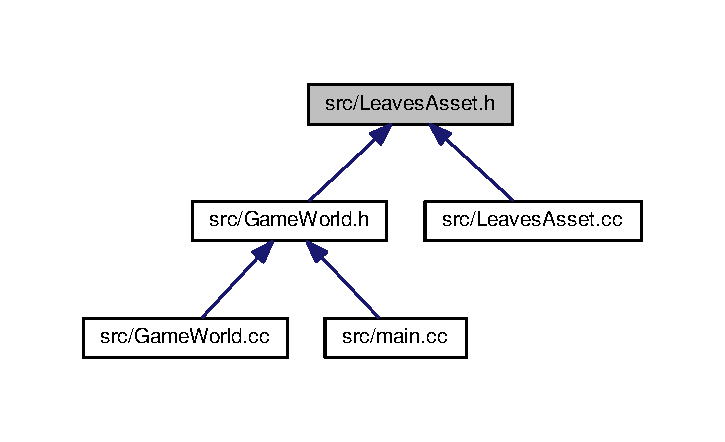
\includegraphics[width=348pt]{LeavesAsset_8h__dep__incl}
\end{center}
\end{figure}
\subsection*{Classes}
\begin{DoxyCompactItemize}
\item 
class \hyperlink{classLeavesAsset}{Leaves\+Asset}
\end{DoxyCompactItemize}

\hypertarget{main_8cc}{}\section{src/main.cc File Reference}
\label{main_8cc}\index{src/main.\+cc@{src/main.\+cc}}
{\ttfamily \#include $<$G\+L/glew.\+h$>$}\\*
{\ttfamily \#include $<$S\+D\+L2/\+S\+D\+L.\+h$>$}\\*
{\ttfamily \#include $<$iostream$>$}\\*
{\ttfamily \#include $<$memory$>$}\\*
{\ttfamily \#include $<$boost/program\+\_\+options.\+hpp$>$}\\*
{\ttfamily \#include \char`\"{}common.\+h\char`\"{}}\\*
{\ttfamily \#include \char`\"{}Game\+World.\+h\char`\"{}}\\*
Include dependency graph for main.\+cc\+:\nopagebreak
\begin{figure}[H]
\begin{center}
\leavevmode
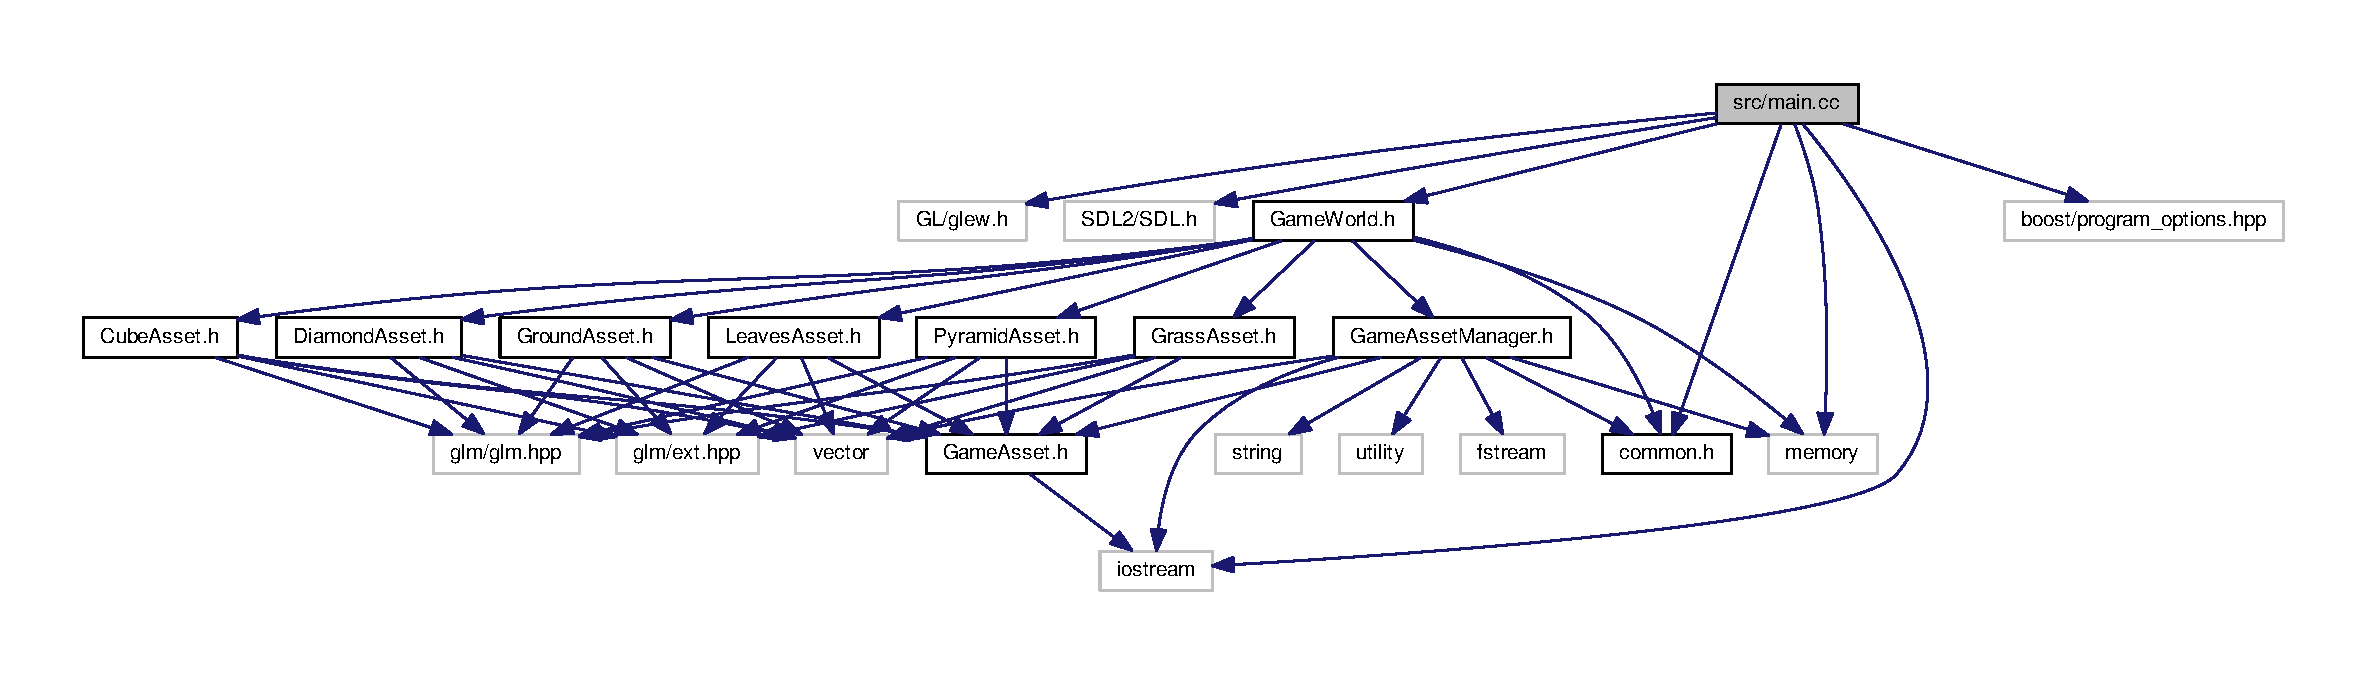
\includegraphics[width=350pt]{main_8cc__incl}
\end{center}
\end{figure}
\subsection*{Classes}
\begin{DoxyCompactItemize}
\item 
struct \hyperlink{structSDLWindowDeleter}{S\+D\+L\+Window\+Deleter}
\end{DoxyCompactItemize}
\subsection*{Macros}
\begin{DoxyCompactItemize}
\item 
\#define \hyperlink{main_8cc_abcde84ea0ef5f934384e4620f092c85a}{G\+L\+E\+W\+\_\+\+S\+T\+A\+T\+I\+C}
\item 
\#define \hyperlink{main_8cc_a6ff0ea1b288e03115f981ba31f96fade}{R\+U\+N\+\_\+\+G\+R\+A\+P\+H\+I\+C\+S\+\_\+\+D\+I\+S\+P\+L\+A\+Y}~0x00;
\end{DoxyCompactItemize}
\subsection*{Functions}
\begin{DoxyCompactItemize}
\item 
Uint32 \hyperlink{main_8cc_a70eaa727262f633037c3f4b7d3ff24c2}{tick} (Uint32 interval, void $\ast$param)
\begin{DoxyCompactList}\small\item\em S\+D\+L timers run in separate threads. \end{DoxyCompactList}\item 
void \hyperlink{main_8cc_ae1fc7acb89acd89e2d93d844387f73a8}{Draw} (const std\+::shared\+\_\+ptr$<$ S\+D\+L\+\_\+\+Window $>$ \&window, const std\+::shared\+\_\+ptr$<$ \hyperlink{classGameWorld}{Game\+World} $>$ \&game\+\_\+world)
\item 
std\+::shared\+\_\+ptr$<$ S\+D\+L\+\_\+\+Window $>$ \hyperlink{main_8cc_acab7ade71cf38099442ca5df2495223d}{Init\+World} ()
\item 
\hyperlink{common_8h_add86e7c88dd109abea3f708b422f31f0}{Application\+Mode} \hyperlink{main_8cc_aba227fab3b52f0ce7c5b89d75b88dcdc}{Parse\+Options} (int argc, char $\ast$$\ast$argv)
\item 
int \hyperlink{main_8cc_a3c04138a5bfe5d72780bb7e82a18e627}{main} (int argc, char $\ast$$\ast$argv)
\end{DoxyCompactItemize}


\subsection{Macro Definition Documentation}
\hypertarget{main_8cc_abcde84ea0ef5f934384e4620f092c85a}{}\index{main.\+cc@{main.\+cc}!G\+L\+E\+W\+\_\+\+S\+T\+A\+T\+I\+C@{G\+L\+E\+W\+\_\+\+S\+T\+A\+T\+I\+C}}
\index{G\+L\+E\+W\+\_\+\+S\+T\+A\+T\+I\+C@{G\+L\+E\+W\+\_\+\+S\+T\+A\+T\+I\+C}!main.\+cc@{main.\+cc}}
\subsubsection[{G\+L\+E\+W\+\_\+\+S\+T\+A\+T\+I\+C}]{\setlength{\rightskip}{0pt plus 5cm}\#define G\+L\+E\+W\+\_\+\+S\+T\+A\+T\+I\+C}\label{main_8cc_abcde84ea0ef5f934384e4620f092c85a}
\hypertarget{main_8cc_a6ff0ea1b288e03115f981ba31f96fade}{}\index{main.\+cc@{main.\+cc}!R\+U\+N\+\_\+\+G\+R\+A\+P\+H\+I\+C\+S\+\_\+\+D\+I\+S\+P\+L\+A\+Y@{R\+U\+N\+\_\+\+G\+R\+A\+P\+H\+I\+C\+S\+\_\+\+D\+I\+S\+P\+L\+A\+Y}}
\index{R\+U\+N\+\_\+\+G\+R\+A\+P\+H\+I\+C\+S\+\_\+\+D\+I\+S\+P\+L\+A\+Y@{R\+U\+N\+\_\+\+G\+R\+A\+P\+H\+I\+C\+S\+\_\+\+D\+I\+S\+P\+L\+A\+Y}!main.\+cc@{main.\+cc}}
\subsubsection[{R\+U\+N\+\_\+\+G\+R\+A\+P\+H\+I\+C\+S\+\_\+\+D\+I\+S\+P\+L\+A\+Y}]{\setlength{\rightskip}{0pt plus 5cm}\#define R\+U\+N\+\_\+\+G\+R\+A\+P\+H\+I\+C\+S\+\_\+\+D\+I\+S\+P\+L\+A\+Y~0x00;}\label{main_8cc_a6ff0ea1b288e03115f981ba31f96fade}


\subsection{Function Documentation}
\hypertarget{main_8cc_ae1fc7acb89acd89e2d93d844387f73a8}{}\index{main.\+cc@{main.\+cc}!Draw@{Draw}}
\index{Draw@{Draw}!main.\+cc@{main.\+cc}}
\subsubsection[{Draw(const std\+::shared\+\_\+ptr$<$ S\+D\+L\+\_\+\+Window $>$ \&window, const std\+::shared\+\_\+ptr$<$ Game\+World $>$ \&game\+\_\+world)}]{\setlength{\rightskip}{0pt plus 5cm}void Draw (
\begin{DoxyParamCaption}
\item[{const std\+::shared\+\_\+ptr$<$ S\+D\+L\+\_\+\+Window $>$ \&}]{window, }
\item[{const std\+::shared\+\_\+ptr$<$ {\bf Game\+World} $>$ \&}]{game\+\_\+world}
\end{DoxyParamCaption}
)}\label{main_8cc_ae1fc7acb89acd89e2d93d844387f73a8}

\begin{DoxyCode}
50                                                                                                  \{
51   glClearColor(0.0f, 206.0f, 250.0f, 1.0f);
52   glClear(GL\_COLOR\_BUFFER\_BIT|GL\_DEPTH\_BUFFER\_BIT);
53 
54   game\_world->Draw();
55 
56   \textcolor{comment}{// Don't forget to swap the buffers}
57   SDL\_GL\_SwapWindow(window.get());
58 \}
\end{DoxyCode}
\hypertarget{main_8cc_acab7ade71cf38099442ca5df2495223d}{}\index{main.\+cc@{main.\+cc}!Init\+World@{Init\+World}}
\index{Init\+World@{Init\+World}!main.\+cc@{main.\+cc}}
\subsubsection[{Init\+World()}]{\setlength{\rightskip}{0pt plus 5cm}std\+::shared\+\_\+ptr$<$S\+D\+L\+\_\+\+Window$>$ Init\+World (
\begin{DoxyParamCaption}
{}
\end{DoxyParamCaption}
)}\label{main_8cc_acab7ade71cf38099442ca5df2495223d}

\begin{DoxyCode}
60                                       \{
61   Uint32 width = 1280;\textcolor{comment}{//1280;}
62   Uint32 height = 800;\textcolor{comment}{//800;}
63   SDL\_Window * \_window;
64   std::shared\_ptr<SDL\_Window> window;
65   
66 
67   \textcolor{comment}{// Glew will later ensure that OpenGL 3 *is* supported}
68   SDL\_GL\_SetAttribute(SDL\_GL\_CONTEXT\_PROFILE\_MASK, SDL\_GL\_CONTEXT\_PROFILE\_CORE);
69   SDL\_GL\_SetAttribute(SDL\_GL\_CONTEXT\_MAJOR\_VERSION, 3);
70   SDL\_GL\_SetAttribute(SDL\_GL\_CONTEXT\_MINOR\_VERSION, 0);
71 
72   \textcolor{comment}{// Do double buffering in GL}
73   SDL\_GL\_SetAttribute(SDL\_GL\_DOUBLEBUFFER, 1);
74   SDL\_GL\_SetAttribute(SDL\_GL\_DEPTH\_SIZE, 24);
75  
76   \textcolor{comment}{// Initialise SDL - when using C/C++ it's common to have to}
77   \textcolor{comment}{// initialise libraries by calling a function within them.}
78   \textcolor{keywordflow}{if} (SDL\_Init(SDL\_INIT\_VIDEO|SDL\_INIT\_AUDIO|SDL\_INIT\_TIMER)<0) \{
79     std::cout << \textcolor{stringliteral}{"Failed to initialise SDL: "} << SDL\_GetError() << std::endl;
80     \textcolor{keywordflow}{return} \textcolor{keyword}{nullptr};
81   \}
82 
83   \textcolor{comment}{// When we close a window quit the SDL application}
84   atexit(SDL\_Quit);
85 
86   \textcolor{comment}{// Create a new window with an OpenGL surface}
87   \_window = SDL\_CreateWindow(\textcolor{stringliteral}{"Shader Example"}
88                              , SDL\_WINDOWPOS\_CENTERED
89                              , SDL\_WINDOWPOS\_CENTERED
90                              , width
91                              , height
92                              , SDL\_WINDOW\_OPENGL | SDL\_WINDOW\_SHOWN);
93   \textcolor{keywordflow}{if} (!\_window) \{
94     std::cout << \textcolor{stringliteral}{"Failed to create SDL window: "} << SDL\_GetError() << std::endl;
95     \textcolor{keywordflow}{return} \textcolor{keyword}{nullptr};
96   \}
97 
98   SDL\_GLContext glContext = SDL\_GL\_CreateContext(\_window);
99   \textcolor{keywordflow}{if} (!glContext) \{
100     std::cout << \textcolor{stringliteral}{"Failed to create OpenGL context: "} << SDL\_GetError() << std::endl;
101     \textcolor{keywordflow}{return} \textcolor{keyword}{nullptr};
102   \}
103 
104   \textcolor{comment}{// Initialise GLEW - an easy way to ensure OpenGl 3.0+}
105   \textcolor{comment}{// The *must* be done after we have set the video mode - otherwise we have no}
106   \textcolor{comment}{// OpenGL context to test.}
107   glewInit();
108   \textcolor{keywordflow}{if} (!glewIsSupported(\textcolor{stringliteral}{"GL\_VERSION\_3\_0"})) \{
109     std::cerr << \textcolor{stringliteral}{"OpenGL 3.0 not available"} << std::endl;
110     \textcolor{keywordflow}{return} \textcolor{keyword}{nullptr};
111   \}
112 
113   \textcolor{comment}{// OpenGL settings}
114   glDisable(GL\_CULL\_FACE);
115   glEnable(GL\_DEPTH\_TEST);
116   glDepthFunc(GL\_LESS);
117 
118   window.reset(\_window, SDL\_DestroyWindow);
119   \textcolor{keywordflow}{return} window;
120 \}
\end{DoxyCode}
\hypertarget{main_8cc_a3c04138a5bfe5d72780bb7e82a18e627}{}\index{main.\+cc@{main.\+cc}!main@{main}}
\index{main@{main}!main.\+cc@{main.\+cc}}
\subsubsection[{main(int argc, char $\ast$$\ast$argv)}]{\setlength{\rightskip}{0pt plus 5cm}int main (
\begin{DoxyParamCaption}
\item[{int}]{argc, }
\item[{char $\ast$$\ast$}]{argv}
\end{DoxyParamCaption}
)}\label{main_8cc_a3c04138a5bfe5d72780bb7e82a18e627}
Add the main event loop. Detects Keyboard and Mouse Sends Data to \hyperlink{classGameWorld}{Game\+World} Camera Controls
\begin{DoxyCode}
152                                    \{
153     Uint32 delay = 1000/30; \textcolor{comment}{// in milliseconds, Temporary change to 30fps to fix speed of the game.}
154 
155   \textcolor{keyword}{auto} mode = \hyperlink{main_8cc_aba227fab3b52f0ce7c5b89d75b88dcdc}{ParseOptions}(argc, argv);
156   \textcolor{keyword}{auto} window = \hyperlink{main_8cc_acab7ade71cf38099442ca5df2495223d}{InitWorld}();
157   \textcolor{keyword}{auto} game\_world = std::make\_shared<GameWorld>(mode);
158   \textcolor{keywordflow}{if}(!window) \{
159     SDL\_Quit();
160   \} 
161 
162   \textcolor{comment}{// Call the function "tick" every delay milliseconds}
163   SDL\_AddTimer(delay, \hyperlink{main_8cc_a70eaa727262f633037c3f4b7d3ff24c2}{tick}, NULL);
164 
165         cout << \textcolor{stringliteral}{"****************************************************************************************"} 
      << endl;
166         cout << \textcolor{stringliteral}{"*                                                                                      *"} 
      << endl;
167         cout << \textcolor{stringliteral}{"*                                     Starting Game                                    *"} 
      << endl;
168         cout << \textcolor{stringliteral}{"*                                                                                      *"} 
      << endl;
169         cout << \textcolor{stringliteral}{"*--------------------------------------------------------------------------------------*"} 
      << endl;
170         cout << \textcolor{stringliteral}{"*                                                                                      *"} 
      << endl;
171         cout << \textcolor{stringliteral}{"*                               A simple Minecraft Like Game                           *"} 
      << endl;
172         cout << \textcolor{stringliteral}{"*                        With Block Spawing , Player Movement and                      *"} 
      << endl;
173         cout << \textcolor{stringliteral}{"*                                     Camera Control                                   *"} 
      << endl;
174         cout << \textcolor{stringliteral}{"*                                                                                      *"} 
      << endl;
175         cout << \textcolor{stringliteral}{"*--------------------------------------------------------------------------------------*"} 
      << endl;
176         cout << \textcolor{stringliteral}{"*                                                                                      *"} 
      << endl;
177         cout << \textcolor{stringliteral}{"*                                    Work In Progress                                  *"} 
      << endl;
178         cout << \textcolor{stringliteral}{"*                                                                                      *"} 
      << endl;
179         cout << \textcolor{stringliteral}{"*--------------------------------------------------------------------------------------*"} 
      << endl;
180         cout << \textcolor{stringliteral}{"*                                                                                      *"} 
      << endl;
181         cout << \textcolor{stringliteral}{"*                                       Controls                                       *"} 
      << endl;
182         cout << \textcolor{stringliteral}{"*                                                                                      *"} 
      << endl;
183         cout << \textcolor{stringliteral}{"*                 Player                                      Camera                   *"} 
      << endl;
184         cout << \textcolor{stringliteral}{"*                Forward                                        Up                     *"} 
      << endl;
185         cout << \textcolor{stringliteral}{"*                 \_\_\_\_\_                                        \_\_\_\_\_                   *"} 
      << endl;
186         cout << \textcolor{stringliteral}{"*                |     |                                      |     |                  *"} 
      << endl;
187         cout << \textcolor{stringliteral}{"*                |  w  |                                      |  ^  |                  *"} 
      << endl;
188         cout << \textcolor{stringliteral}{"*                |\_\_\_\_\_|                                      |\_\_\_\_\_|                  *"} 
      << endl;
189         cout << \textcolor{stringliteral}{"*          \_\_\_\_\_  \_\_\_\_\_  \_\_\_\_\_                          \_\_\_\_\_  \_\_\_\_\_  \_\_\_\_\_            *"} 
      << endl;
190         cout << \textcolor{stringliteral}{"*  Player |     ||     ||     | Player         Camera  |     ||     ||     | Camera    *"} 
      << endl;
191         cout << \textcolor{stringliteral}{"*   Left  |  a  ||  s  ||  d  |  Right          Left   |  <  ||  v  ||  >  |  Right    *"} 
      << endl;
192         cout << \textcolor{stringliteral}{"*         |\_\_\_\_\_||\_\_\_\_\_||\_\_\_\_\_|                        |\_\_\_\_\_||\_\_\_\_\_||\_\_\_\_\_|           *"} 
      << endl;
193         cout << \textcolor{stringliteral}{"*                                                                                      *"} 
      << endl;
194         cout << \textcolor{stringliteral}{"*                 Player                                       Camera                  *"} 
      << endl;
195         cout << \textcolor{stringliteral}{"*                Backwards                                      Down                   *"} 
      << endl;
196         cout << \textcolor{stringliteral}{"*                                      Mouse                                           *"} 
      << endl;
197         cout << \textcolor{stringliteral}{"*                                     \_\_\_\_\_\_\_                                          *"} 
      << endl;
198         cout << \textcolor{stringliteral}{"*                                    |    |   |                                        *"} 
      << endl;
199         cout << \textcolor{stringliteral}{"*                                   |     |    |                                       *"} 
      << endl;
200         cout << \textcolor{stringliteral}{"*                                  |      |     |                                      *"} 
      << endl;
201         cout << \textcolor{stringliteral}{"*                                  |      |     |                                      *"} 
      << endl;
202         cout << \textcolor{stringliteral}{"*                                 |              |                                     *"} 
      << endl;
203         cout << \textcolor{stringliteral}{"*                                 |              |                                     *"} 
      << endl;
204         cout << \textcolor{stringliteral}{"*                                 |              |                                     *"} 
      << endl;
205         cout << \textcolor{stringliteral}{"*                                  |            |                                      *"} 
      << endl;
206         cout << \textcolor{stringliteral}{"*                                   |          |                                       *"} 
      << endl;
207         cout << \textcolor{stringliteral}{"*                                    |\_\_\_\_\_\_\_\_|                                        *"} 
      << endl;
208         cout << \textcolor{stringliteral}{"*                                                                                      *"} 
      << endl;
209         cout << \textcolor{stringliteral}{"*                          Camera Control Same as Arrow Keys                           *"} 
      << endl;
210         cout << \textcolor{stringliteral}{"*                                                                                      *"} 
      << endl;
211         cout << \textcolor{stringliteral}{"*                                                                                      *"} 
      << endl;
212         cout << \textcolor{stringliteral}{"*                                                                                      *"} 
      << endl;
213         cout << \textcolor{stringliteral}{"*                               Jump Up                         Drop Down              *"} 
      << endl;
214         cout << \textcolor{stringliteral}{"*           \_\_\_\_\_\_\_\_\_\_\_\_\_\_\_\_\_\_\_\_\_\_\_\_\_\_\_\_\_\_\_\_\_\_\_\_\_\_\_\_\_\_\_\_\_\_     \_\_\_\_\_\_\_\_\_\_\_             *"} 
      << endl;
215         cout << \textcolor{stringliteral}{"*          |                                              |   |           |            *"} 
      << endl;
216         cout << \textcolor{stringliteral}{"*          |                     Space                    |   | -->|(tab) |            *"} 
      << endl;
217         cout << \textcolor{stringliteral}{"*          |\_\_\_\_\_\_\_\_\_\_\_\_\_\_\_\_\_\_\_\_\_\_\_\_\_\_\_\_\_\_\_\_\_\_\_\_\_\_\_\_\_\_\_\_\_\_|   |\_\_\_\_\_\_\_\_\_\_\_|            *"} 
      << endl;
218         cout << \textcolor{stringliteral}{"*                                                                                      *"} 
      << endl;
219         cout << \textcolor{stringliteral}{"*                                                                                      *"} 
      << endl;
220         cout << \textcolor{stringliteral}{"*                                                                                      *"} 
      << endl;
221         cout << \textcolor{stringliteral}{"*                                       Quit Game                                      *"} 
      << endl;
222         cout << \textcolor{stringliteral}{"*                                         \_\_\_\_\_                                        *"} 
      << endl;
223         cout << \textcolor{stringliteral}{"*                                        |     |                                       *"} 
      << endl;
224         cout << \textcolor{stringliteral}{"*                                        | esc |                                       *"} 
      << endl;
225         cout << \textcolor{stringliteral}{"*                                        |\_\_\_\_\_|                                       *"} 
      << endl;
226         cout << \textcolor{stringliteral}{"*                                                                                      *"} 
      << endl;
227         cout << \textcolor{stringliteral}{"*                                                                                      *"} 
      << endl;
228         cout << \textcolor{stringliteral}{"****************************************************************************************"} 
      << endl;
229         cout << \textcolor{stringliteral}{""} << endl;
230 
231     \textcolor{comment}{//SDL\_SetRelativeMouseMode(SDL\_TRUE);      }
232     \textcolor{comment}{//SDL\_GetRelativeMouseState(&X, &Y);}
233 
234         \textcolor{keywordtype}{int} Old\_Mouse\_X;
235         \textcolor{keywordtype}{int} Old\_Mouse\_Y;
236 
237         \textcolor{keywordtype}{int} Mouse\_X;
238         \textcolor{keywordtype}{int} Mouse\_Y;
239 
245   SDL\_Event event;
246   \textcolor{keywordflow}{while} (SDL\_WaitEvent(&event)) \{
247     \textcolor{keywordflow}{switch} (event.type) \{
248     \textcolor{keywordflow}{case} SDL\_QUIT:
249       SDL\_Quit();
250       \textcolor{keywordflow}{break};
251     \textcolor{keywordflow}{case} SDL\_USEREVENT:
252       \hyperlink{main_8cc_ae1fc7acb89acd89e2d93d844387f73a8}{Draw}(window, game\_world);
253       \textcolor{keywordflow}{break};
254     \textcolor{keywordflow}{case}  SDL\_MOUSEMOTION:
255         \textcolor{comment}{// save old mouse coordinates X}
256         Old\_Mouse\_X = Mouse\_X;
257         \textcolor{comment}{// get mouse coordinates X}
258         Mouse\_X = \textcolor{keyword}{event}.motion.x;
259         
260       \textcolor{keywordflow}{if} (Mouse\_X > Old\_Mouse\_X) \{             \textcolor{comment}{// Mouse move Right}
261               game\_world -> Camera\_Control(\textcolor{charliteral}{'>'});
262       \}
263       \textcolor{keywordflow}{else} \textcolor{keywordflow}{if} (Mouse\_X < Old\_Mouse\_X) \{        \textcolor{comment}{// Mouse move Left}
264               game\_world -> Camera\_Control(\textcolor{charliteral}{'<'});
265       \}
266         \textcolor{comment}{// save old mouse coordinates Y}
267         Old\_Mouse\_Y = Mouse\_Y;
268         \textcolor{comment}{// get mouse coordinates Y}
269         Mouse\_Y = \textcolor{keyword}{event}.motion.y;
270       \textcolor{keywordflow}{if} (Mouse\_Y < Old\_Mouse\_Y) \{             \textcolor{comment}{// Mouse move Up }
271               game\_world -> Camera\_Control(\textcolor{charliteral}{'^'});
272       \}
273       \textcolor{keywordflow}{else} \textcolor{keywordflow}{if} (Mouse\_Y > Old\_Mouse\_Y) \{ \textcolor{comment}{// Mouse move Down}
274               game\_world -> Camera\_Control(\textcolor{charliteral}{'v'});
275       \}
276       \textcolor{keywordflow}{break};
277     \textcolor{keywordflow}{case} SDL\_KEYDOWN:           \textcolor{comment}{// At keyboard press}
278     \textcolor{keywordflow}{switch} (event.key.keysym.sym) \{
279     \textcolor{keywordflow}{case} SDLK\_ESCAPE:           \textcolor{comment}{// when pressing q}
280     SDL\_Quit();         \textcolor{comment}{// Quit program}
281     cout << \textcolor{stringliteral}{"Key 'q' Pressed, Game closed"} << endl;
282     \textcolor{keywordflow}{break};
283     \textcolor{keywordflow}{case} SDLK\_w:            \textcolor{comment}{// When pressing w}
284         game\_world -> Camera\_Control(\textcolor{charliteral}{'w'});
285       \textcolor{keywordflow}{break};
286     \textcolor{keywordflow}{case} SDLK\_a:            \textcolor{comment}{// When pressing a}
287         game\_world -> Camera\_Control(\textcolor{charliteral}{'a'});
288       \textcolor{keywordflow}{break};
289     \textcolor{keywordflow}{case} SDLK\_s:            \textcolor{comment}{// When pressing s}
290         game\_world -> Camera\_Control(\textcolor{charliteral}{'s'});
291       \textcolor{keywordflow}{break};
292     \textcolor{keywordflow}{case} SDLK\_d:            \textcolor{comment}{// When pressing d}
293         game\_world -> Camera\_Control(\textcolor{charliteral}{'d'});
294       \textcolor{keywordflow}{break};
295     \textcolor{keywordflow}{case} SDLK\_UP:           \textcolor{comment}{// When pressing Arrow Up}
296         game\_world -> Camera\_Control(\textcolor{charliteral}{'^'});
297       \textcolor{keywordflow}{break};
298     \textcolor{keywordflow}{case} SDLK\_LEFT:         \textcolor{comment}{// When pressing Arrow Left}
299         game\_world -> Camera\_Control(\textcolor{charliteral}{'<'});
300       \textcolor{keywordflow}{break};
301     \textcolor{keywordflow}{case} SDLK\_DOWN:         \textcolor{comment}{// When pressing Arrow down}
302         game\_world -> Camera\_Control(\textcolor{charliteral}{'v'});
303       \textcolor{keywordflow}{break};
304     \textcolor{keywordflow}{case} SDLK\_RIGHT:            \textcolor{comment}{// When pressing Arrow right}
305         game\_world -> Camera\_Control(\textcolor{charliteral}{'>'});
306       \textcolor{keywordflow}{break};
307     \textcolor{keywordflow}{case} SDLK\_SPACE:                    \textcolor{comment}{// When pressing Space Go Up}
308         game\_world -> Camera\_Control(\textcolor{charliteral}{'+'});
309       \textcolor{keywordflow}{break};
310     \textcolor{keywordflow}{case} SDLK\_TAB:                      \textcolor{comment}{// When pressing Tab Go Down}
311         game\_world -> Camera\_Control(\textcolor{charliteral}{'-'});
312     \textcolor{keywordflow}{default}:
313       \textcolor{keywordflow}{break};
314       \}
315     \}
316   \}
317 \}
\end{DoxyCode}
\hypertarget{main_8cc_aba227fab3b52f0ce7c5b89d75b88dcdc}{}\index{main.\+cc@{main.\+cc}!Parse\+Options@{Parse\+Options}}
\index{Parse\+Options@{Parse\+Options}!main.\+cc@{main.\+cc}}
\subsubsection[{Parse\+Options(int argc, char $\ast$$\ast$argv)}]{\setlength{\rightskip}{0pt plus 5cm}{\bf Application\+Mode} Parse\+Options (
\begin{DoxyParamCaption}
\item[{int}]{argc, }
\item[{char $\ast$$\ast$}]{argv}
\end{DoxyParamCaption}
)}\label{main_8cc_aba227fab3b52f0ce7c5b89d75b88dcdc}

\begin{DoxyCode}
122                                                       \{
123   \textcolor{keyword}{namespace }po = boost::program\_options;
124 
125   po::options\_description desc(\textcolor{stringliteral}{"Allowed options"});
126   desc.add\_options()
127      (\textcolor{stringliteral}{"help"}, \textcolor{stringliteral}{"print this help message"})
128      (\textcolor{stringliteral}{"translate"}, \textcolor{stringliteral}{"Show translation example (default)"})
129      (\textcolor{stringliteral}{"rotate"}, \textcolor{stringliteral}{"Show rotation example"})
130      (\textcolor{stringliteral}{"scale"}, \textcolor{stringliteral}{"Show scale example"})
131   ;
132 
133   po::variables\_map vm;
134   po::store(po::parse\_command\_line(argc, argv, desc), vm);
135   po::notify(vm);
136 
137   \textcolor{keywordflow}{if}(vm.count(\textcolor{stringliteral}{"help"})) \{
138     std::cout << desc << std::endl;
139     exit(0);
140   \}
141 
142   \textcolor{keywordflow}{if}(vm.count(\textcolor{stringliteral}{"rotate"})) \{
143     \textcolor{keywordflow}{return} \hyperlink{common_8h_add86e7c88dd109abea3f708b422f31f0a3dcfe0046eb5876e287dbf0914819b16}{ROTATE};
144   \}
145 
146   \textcolor{keywordflow}{if}(vm.count(\textcolor{stringliteral}{"scale"})) \{
147     \textcolor{keywordflow}{return} \hyperlink{common_8h_add86e7c88dd109abea3f708b422f31f0a593be05a10070b4e7e0856e20590eaaf}{SCALE};
148   \}
149   \textcolor{comment}{// The default}
150   \textcolor{keywordflow}{return} \hyperlink{common_8h_add86e7c88dd109abea3f708b422f31f0a25f73324dc93d9024c0c75b4e6815335}{TRANSFORM};
151 \}
\end{DoxyCode}
\hypertarget{main_8cc_a70eaa727262f633037c3f4b7d3ff24c2}{}\index{main.\+cc@{main.\+cc}!tick@{tick}}
\index{tick@{tick}!main.\+cc@{main.\+cc}}
\subsubsection[{tick(\+Uint32 interval, void $\ast$param)}]{\setlength{\rightskip}{0pt plus 5cm}Uint32 tick (
\begin{DoxyParamCaption}
\item[{Uint32}]{interval, }
\item[{void $\ast$}]{param}
\end{DoxyParamCaption}
)}\label{main_8cc_a70eaa727262f633037c3f4b7d3ff24c2}


S\+D\+L timers run in separate threads. 

In the timer thread push an event onto the event queue. This event signifies to call display() from the thread in which the Open\+G\+L context was created. 
\begin{DoxyCode}
34                                           \{
35   SDL\_Event event;
36   \textcolor{keyword}{event}.type = SDL\_USEREVENT;
37   \textcolor{keyword}{event}.user.code = \hyperlink{main_8cc_a6ff0ea1b288e03115f981ba31f96fade}{RUN\_GRAPHICS\_DISPLAY};
38   \textcolor{keyword}{event}.user.data1 = 0;
39   \textcolor{keyword}{event}.user.data2 = 0;
40   SDL\_PushEvent(&event);
41   \textcolor{keywordflow}{return} interval;
42 \}
\end{DoxyCode}

\hypertarget{PyramidAsset_8cc}{}\section{src/\+Pyramid\+Asset.cc File Reference}
\label{PyramidAsset_8cc}\index{src/\+Pyramid\+Asset.\+cc@{src/\+Pyramid\+Asset.\+cc}}
{\ttfamily \#include \char`\"{}Pyramid\+Asset.\+h\char`\"{}}\\*
\subsection*{Macros}
\begin{DoxyCompactItemize}
\item 
\#define \hyperlink{PyramidAsset_8cc_a75f201b0e53e68726854997957322b8d}{check\+G\+L\+Error}()
\end{DoxyCompactItemize}


\subsection{Macro Definition Documentation}
\hypertarget{PyramidAsset_8cc_a75f201b0e53e68726854997957322b8d}{}\index{Pyramid\+Asset.\+cc@{Pyramid\+Asset.\+cc}!check\+G\+L\+Error@{check\+G\+L\+Error}}
\index{check\+G\+L\+Error@{check\+G\+L\+Error}!Pyramid\+Asset.\+cc@{Pyramid\+Asset.\+cc}}
\subsubsection[{check\+G\+L\+Error}]{\setlength{\rightskip}{0pt plus 5cm}\#define check\+G\+L\+Error(
\begin{DoxyParamCaption}
{}
\end{DoxyParamCaption}
)}\label{PyramidAsset_8cc_a75f201b0e53e68726854997957322b8d}

\hypertarget{PyramidAsset_8h}{}\section{src/\+Pyramid\+Asset.h File Reference}
\label{PyramidAsset_8h}\index{src/\+Pyramid\+Asset.\+h@{src/\+Pyramid\+Asset.\+h}}
{\ttfamily \#include $<$vector$>$}\\*
{\ttfamily \#include $<$glm/glm.\+hpp$>$}\\*
{\ttfamily \#include $<$glm/ext.\+hpp$>$}\\*
{\ttfamily \#include \char`\"{}Game\+Asset.\+h\char`\"{}}\\*
Include dependency graph for Pyramid\+Asset.\+h\+:\nopagebreak
\begin{figure}[H]
\begin{center}
\leavevmode
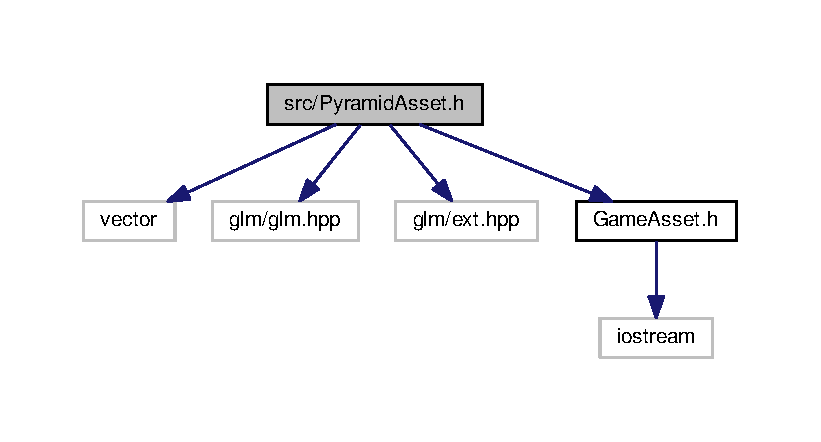
\includegraphics[width=350pt]{PyramidAsset_8h__incl}
\end{center}
\end{figure}
This graph shows which files directly or indirectly include this file\+:\nopagebreak
\begin{figure}[H]
\begin{center}
\leavevmode
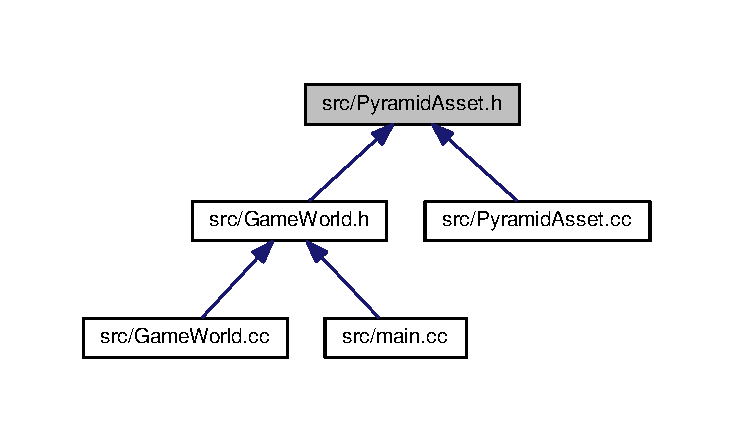
\includegraphics[width=350pt]{PyramidAsset_8h__dep__incl}
\end{center}
\end{figure}
\subsection*{Classes}
\begin{DoxyCompactItemize}
\item 
class \hyperlink{classPyramidAsset}{Pyramid\+Asset}
\end{DoxyCompactItemize}

%--- End generated contents ---

% Index
\backmatter
\newpage
\phantomsection
\clearemptydoublepage
\addcontentsline{toc}{chapter}{Index}
\printindex

\end{document}
